% pyFormex manual (we use the python manual class)
% $Id$
% (C) B.Verhegghe
%
\documentclass[a4paper]{manual}
%
%% Dirty hack to make Python classes work together with hyperref
\let\pyurl\url
\let\url\relax
%%
\usepackage{a4wide}
\usepackage{times}
\usepackage[T1]{fontenc}
\usepackage[english]{babel}
\usepackage{makeidx}
\usepackage[latex2html,colorlinks,linkcolor=blue]{hyperref}
\usepackage{html}
\usepackage{graphicx}
%\usepackage{subfigure}
\usepackage{verbatim}
\usepackage{units}
%%%
%%% !! \xspace in de URLs geeft problemen met nieuwe TeXLive 2007 !
%%%
%%% xspace.sty v1.06 werkt goed! v1.12 niet!
%%%
\usepackage{xspace}

%%%%%%%%%%%%%%%%%%%%%%%%%%%%%%%%%%%%%%%%%%%%%%%%%%%%%%%%%%%%%%%%%%%%%%%%%%
% Document identification
%%%%%%%%%%%%%%%%%%%%%%%%%%%
\newcommand{\thetitle}{pyFormex manual}
\newcommand{\theauthor}{Benedict Verhegghe}

\title{\pyformex manual}
\author{Benedict Verhegghe}
%\authoraddress{
%	\strong{Python Software Foundation}\\
%	Email: \email{benedict.verhegghe@ugent.be}
%}

% pyFormex version
\renewcommand{\releasename}{pyFormex}
\release{0.7.3-a4}
\setshortversion{0.7.3}
\newcommand{\pyfversion}{pyFormex \version}
%% In the text use \version to refer to the version string only,
%% or \pyfversion to refer to  pyFormex + version string 

%%% !! We should put a fixed date here on releasing final versions !
\date{\today{}}

% pyFormex and its websites
\ifhtml
\newcommand{\pyformex}{pyFormex~}
\newcommand{\pyFormex}{\pyformex}  % we tend to mistype this one!
\newcommand{\pyf}{\pyformex} % saves some typing (and mistyping)
\else
\newcommand{\pyformex}{pyFormex\xspace}
\newcommand{\pyFormex}{\pyformex}  % we tend to mistype this one!
\newcommand{\pyf}{\pyformex} % saves some typing (and mistyping)
\fi

% \newcommand{\pyformex}{pyFormex\xspace}
% \newcommand{\pyFormex}{\pyformex}  % we tend to mistype this one!
% \newcommand{\pyf}{\pyformex} % saves some typing (and mistyping)
% \begin{htmlonly}
% \renewcommand{\pyformex}{pyFormex~}
% \renewcommand{\pyFormex}{\pyformex}  % we tend to mistype this one!
% \renewcommand{\pyf}{\pyformex} % saves some typing (and mistyping)
% \end{htmlonly}


\newcommand{\websiteURL}{http://pyformex.berlios.de\xspace}
\newcommand{\pydocpages}{http://pyformex.berlios.de/doc/index.html\xspace}
\newcommand{\pythonURL}{http://www.python.org\xspace}
\newcommand{\pythonTUT}{http://docs.python.org/tut/\xspace}
\newcommand{\pythonBEG}{http://wiki.python.org/moin/BeginnersGuide/\xspace}
\newcommand{\numpyURL}{http://numpy.scipy.org/\xspace}
\newcommand{\numpyTUT}{http://www.scipy.org/Tentative_NumPy_Tutorial\xspace}
\newcommand{\latestpyf}{http://prdownload.berlios.de/pyformex/pyformex.tar.gz\xspace}
\newcommand{\bumpsFTPserver}{ftp://bumps.ugent.be/pub/pyformex\xspace}

\latex{\hypersetup{
pdfauthor = {\theauthor},
pdftitle = {\thetitle},
pdfsubject = {Tutorial, User Guide and Reference Manual
 for the pyFormex software (\websiteURL)},
pdfkeywords = {3D geometry, 3D surface, finite elements},
%pdfcreator = {},
%pdfproducer = {},
}}

%%%%%%%%%%%%%%%%%%%%%%%%%%%%%%%%%%%%%%%%%%%%%%%%%%%%%%%%%%%%%%%%%%%%%%%%%%%%
% Document formatting
%%%%%%%%%%%%%%%%%%%%%%%%
% \usepackage{fancyhdr}
% \pagestyle{plain}
% \fancyhead{}
% \fancyfoot{}
% \lhead[\sf\leftmark]{}
% \rhead[]{\sf\rightmark}
% \lfoot[\sf\thepage]{}
% \rfoot[]{\sf\thepage}


%%% Provide more space for figures
\setcounter{topnumber}{2}
\renewcommand{\topfraction}{1}% BV : figures may fill complete page
\setcounter{bottomnumber}{1}
\renewcommand{\bottomfraction}{1}% BV
\setcounter{totalnumber}{3}
\renewcommand{\textfraction}{0}% BV
\renewcommand{\floatpagefraction}{.9}% BV
\setcounter{dbltopnumber}{2}
\renewcommand{\dbltopfraction}{1}% BV
\renewcommand{\dblfloatpagefraction}{.9}% BV


% code 
% The following is just for illustration how to include code.
% Do not uncomment: it will not work. Directly use the definitions instead.
\newcommand{\Code}[1]{\texttt{\small #1}}
\newcommand{\CodeLine}[1]{\\\texttt{~~~#1}\\}
%\newenvironment{CodePart}{\begin{verbatim}}{\end{verbatim}}
%\newcommand{\CodeFile}[1]{\verbatiminput{#1}}
\newcommand{\Todo}[1]{\begin{quotation}\emph{#1}\end{quotation}}

\newcommand{\outdated}{\warning{This section is outdated.}}
\newcommand{\worktodo}[1]{\note{#1}}


\newcommand{\classmethod}{\emph{This is a class method, not an instance method.}}

% Create index entries
\makeindex

%%%%%%%%%%%%%%%%%%%%%%%%%%%% document start here %%%%%%%%%%%%%%%%%%%%%
\begin{document}
\maketitle
\thispagestyle{empty}
\begin{latexonly}
  \tableofcontents
\end{latexonly}
%\upshape    % For some reason, the html text defaults to italic
% pyformex manual --- front matter
% $Id$
% (C) B.Verhegghe

% This makes the contents more accessible from the front page of the HTML.
\ifhtml
\chapter*{Front Matter}\label{front}
\else
\begin{abstract}
\fi

\noindent
This document is to become the \pyformex manual. As the \pyformex program itself is still under development, this document is by no means final and does not even pretend to be accurate for any version of \pyformex. 
However, since partial documentation is better than none, we decided to make this preliminary version available to the general public. This document may evolve fast, so check back regularly.
For the most recent information and for topics that are not yet covered in this manual, we refer the user to the \htmladdnormallinkfoot{pydoc pages}{\pydocpages} that were automatically generated from the \pyformex source.\\\\
The contributors to this manual are Benedict Verhegghe, Tim Neels, Matthieu De Beule and Peter Mortier.
\ifhtml
\else
\end{abstract}
\fi

%%% Local Variables: 
%%% mode: latex
%%% TeX-master: "pyformex"
%%% End: 

% pyformex manual --- introduction
% $Id$
% (C) B.Verhegghe

\chapter{Introduction}
\label{cha:introduction}

\ifhtml\begin{abstract}\fi
\noindent
This section explains shortly what \pyformex is and what it is not. It sets the conditions under which you are allowed to use, modify and distribute the program. Next is a list of prerequisite software parts that you need to have installed in order to be able to run this program. We explain how to download and install \pyformex. Finally, you'll find out what basic knowledge you should have in order to understand the tutorial and succesfully use \pyformex. 
\ifhtml\end{abstract}\fi


\section{What is \pyformex?}
\label{sec:what-pyformex}

You probably expect to find here a short definition of what \pyformex is and what it can do for you. I may have to disappoint you: describing the essence of \pyformex in a few lines is not an easy task to do, because the program can be (and is being) used for very different tasks. So I will give you two answers here: a short one and a long one.

The short answer is that \pyformex is a program to \emph{generate large structured sets of coordinates by means of subsequent mathematical transformations gathered in a script.}
If you find this definition too dull, incomprehensible or just not descriptive enough, read on through this section and look at some of the examples in this manual and on the \htmladdnormallinkfoot{\pyformex website}{\websiteURL}. You will then probably have a better idea of what \pyformex{} is. 

The initial intent of \pyformex was the rapid design of three-dimensional structures with a geometry that can easier be obtained through mathematical description than through interactive generation of its subparts and assemblage thereof. While during development of the program we have concentrated mostly on wireframe type structures, surface and solid elements have been part of \pyformex right from the beginning. Still, most of the examples included with \pyformex are of frame type and most of the practical use of the program is in this area. There is also an extensive plugin for working with triangulated surfaces.

The stent\footnote{A stent is a tube-shaped structure that is e.g. used to reopen (and keep open) obstructed blood vessels.} structure in the figure~\ref{fig:WireStent-example} is a good illustration of what \pyformex can do and what it was intended for. It is one of the many examples provided with \pyf.

\begin{figure}[ht]
  \centering
  \begin{makeimage}
  \end{makeimage}
  \begin{latexonly}
    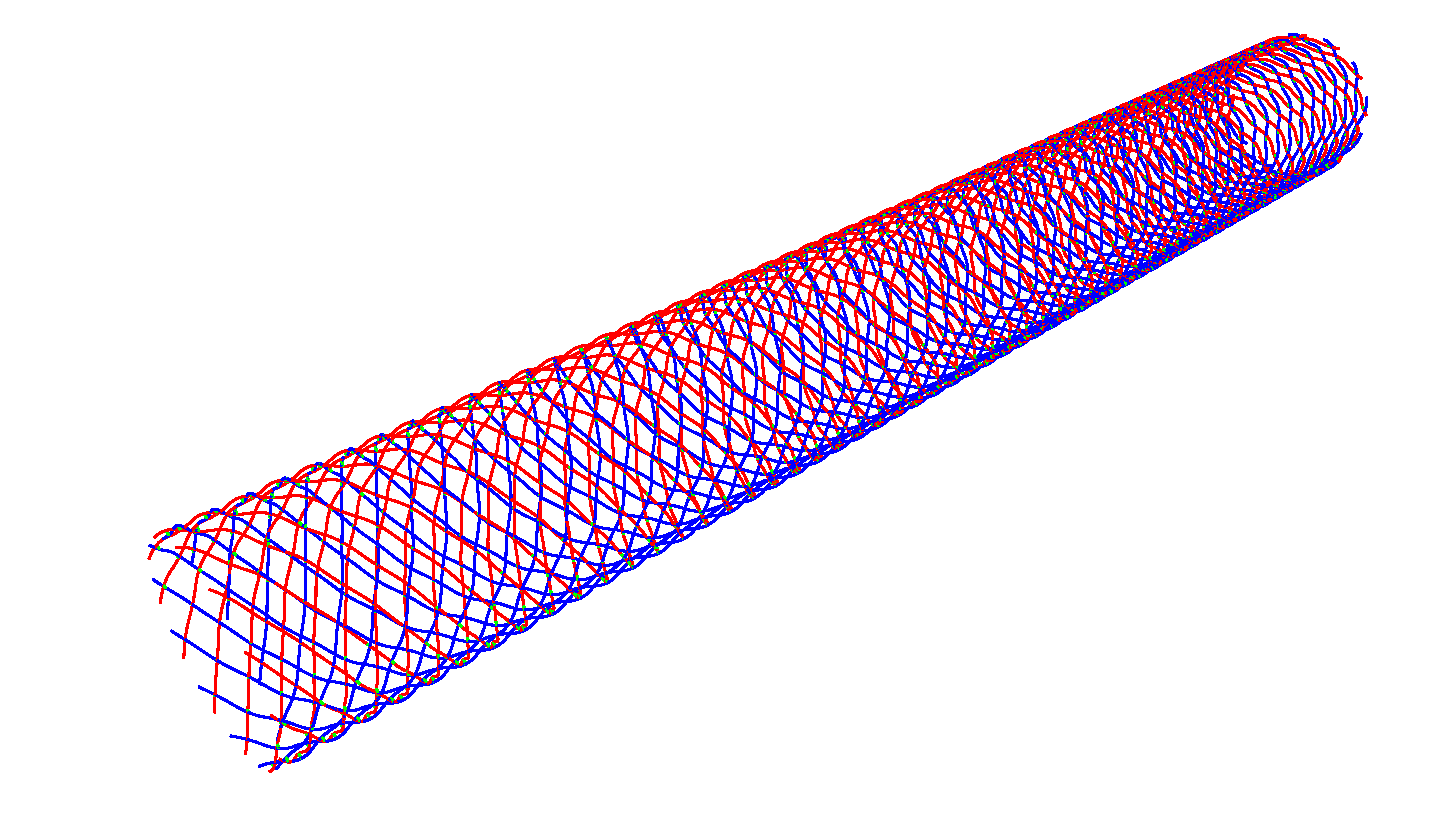
\includegraphics[width=12cm]{images/wirestent}
  \end{latexonly}
  \begin{htmlonly}
    \htmladdimg{../images/wirestent.png}
  \end{htmlonly}  
  \caption{WireStent example.}   \label{fig:WireStent-example}

\end{figure}

The structure is composed of 22032 line segments, each defined by 2 points. Nobody in his right mind would ever even try to input all the 132192 coordinates of all the points describing that structure. 
With \pyformex, one could define the structure by the following sequence of operations, illustrated in the figure~\ref{fig:WireStent-steps}:
 \begin{itemize}
 \item Create a nearly planar base module of two crossing wires. (The wires have a slight out-of-plane bend, to enable the crossing.) 
 \item Extend the base module with a mirrored and translated copy.
 \item Replicate the base module in both directions of the base plane.
 \item Roll the planar grid into a cylinder.
 \end{itemize}
\pyf provides all the needed operations to define the geometry in this way.
 \begin{figure}[ht]
   \centering
   \begin{makeimage}
   \end{makeimage}
   \begin{latexonly}
     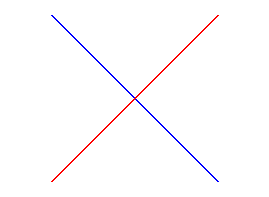
\includegraphics[width=2cm]{images/wirestent-1}\\
     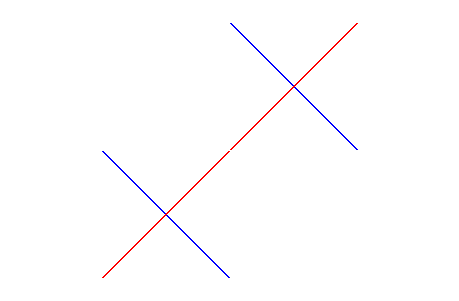
\includegraphics[width=2cm]{images/wirestent-2}\\
     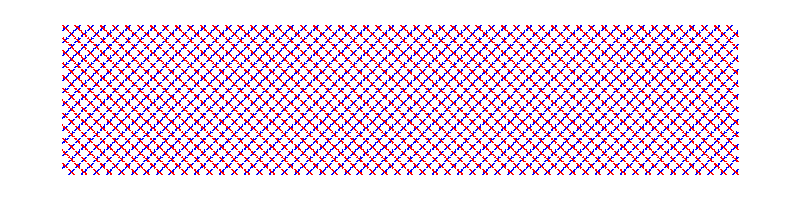
\includegraphics[width=12cm]{images/wirestent-3}
   \end{latexonly}
   \begin{htmlonly}
     \htmladdimg{../images/wirestent-1.png}
     \htmladdimg{../images/wirestent-2.png}
     \htmladdimg{../images/wirestent-3.png}
   \end{htmlonly}  
   \caption{Steps in building the WireStent example.}   \label{fig:WireStent-steps}

 \end{figure}


%\section{Rationale}
%\label{sec:rationale}
\pyformex does not fit into a single category of traditional (mostly commercial) software packages, because it is not being developed as a program with a specific purpose, but rather as a collection of tools and scripts which we needed at some point in our research projects. Many of the tasks for which we now use \pyformex could be done also with some other software package, like a CAD program %(e.g. SolidWorks\textregistered)
or a %(MatLab\textregistered{} style)
matrix calculation package or a solid modeler/renderer %genre Blender
or a finite element pre- and postprocessor%(such as GiD)
. Each of these is very well suited for the task it was designed for, but none provides all the features of \pyformex in a single consistent environment, and certainly not as free software. 

Perhaps the most important feature of \pyformex is that it was primarily intended to be an easy scripting language for creating geometrical models of 3D-structures. The Graphical User Interface was only added as a convenient means to visualize the designed structure. \pyformex can still run without user interface, and this makes it ideal for use in a batch toolchain.

The author of \pyformex, professor in structural engineering and heavy computer user since mainframe times, deeply regrets that computing skills of nowadays engineering students are often limited to using graphical interfaces of mostly commercial packages. This greatly limits their skills, because in their way of thinking: 'If there is no menu item to do some task, then it can not be done!'
The hope to get some of them back into coding has been a stimulus in continuing our work on \pyformex. 
 
Finally, \pyformex is, and will always be, free software in both meanings of free: guaranteeing your freedom (see \ref{sec:license}) and without charging a fee for it. 


%\section{History}
%\label{sec:history}

\section{License and Disclaimer}
\label{sec:license}
\pyformex is \copyright 2004-2007 Benedict Verhegghe

This program is free software; you can redistribute it and/or modify
it under the terms of the \htmladdnormallinkfoot{GNU General Public License}{http://www.gnu.org/licenses/gpl.html} as published by
the Free Software Foundation; either version 2 of the License, or
(at your option) any later version. 

Full details of the license are available in appendix \ref{cha:license} and in the file \textsf{COPYING} included with the distribution. 

This program is distributed in the hope that it will be useful,
but WITHOUT ANY WARRANTY; without even the implied warranty of
MERCHANTABILITY or FITNESS FOR A PARTICULAR PURPOSE.  See the
GNU General Public License for more details.


\section{Installation}
\label{sec:installation}
\subsection{Prerequisites}
\label{sec:prerequisites}
In order to run \pyformex, you need to have the following installed (and working) on your computer.
\begin{itemize}
\item \htmladdnormallinkfoot{Python}{\pythonURL}: Version 2.4 or higher is recommended. Versions 2.3 and 2.2 might work with only a few minor changes.
Nearly all Linux distributions come with Python installed, so this should not be no major obstacle.
\item \htmladdnormallinkfoot{NumPy}{\numpyURL}: Version 1.0-rc1 or higher. Earlier versions can be made to work, but will require some changes to be made. NumPy is the package used for fast numerical array operations in Python and is essential for \pyformex.\footnote{The \texttt{Numarray} package, which was used up until \pyformex 0.3, is no longer supported }
On Linux systems, installing NumPy from source is usually straightforward. Debian users can install the packages python-numpy, python-numpy-dev and python-numpy-ext. There are binary packages for Windows on the \htmladdnormallinkfoot{Sourceforge download page}{http://www.numpy.org/}.
\end{itemize}
If you only want to use the Formex data model and transformation methods, the above will suffice. But most probably you will also want to run the \pyformex Graphical User Interface (GUI) for visualizing your structures. Then you also need the following. 
\begin{itemize}
\item \htmladdnormallinkfoot{Qt4}{http://www.trolltech.com/products/qt}: The widget toolkit on which the GUI was built. For Debian users this  comes in the packages python-qt4 and python-qt4-dev.
\item \htmladdnormallinkfoot{PyQt4}{http://www.riverbankcomputing.co.uk/pyqt/index.php}: The Python bindings for Qt4. Debian users should install the packages python-qt4, python-qt4-dev and python-qt4-gl.
\item \htmladdnormallinkfoot{PyOpenGL}{http://pyopengl.sourceforge.net/}: Python bindings for OpenGL, used for drawing and manipulating the 3D-structures. For debian users this is in the package python-opengl.
\end{itemize}



\subsection{Downloading}
\label{sec:downloading}
The official releases of \pyformex can be downloaded from the 
\htmladdnormallinkfoot{\pyformex website}{\websiteURL}. As of the writing of this manual, the latest release is \htmladdnormallinkfoot{\pyfversion}{\latestpyf}. 
\pyformex is currently distributed in the form of a \Code{.tar.gz} (tarball) archive. See \ref{sec:installation-linux} for how to proceed further.

Alternatively you can download the tarball releases from our \htmladdnormallinkfoot{local FTP server}{\bumpsFTPserver}. The server may be slower, but occasionally you can find there an interim release or release candidate not (yet) available on the official server.

Finally, you can also get the latest development code from the SVN repository on the \htmladdnormallinkfoot{\pyformex website}{\websiteURL}. If you have \htmladdnormallinkfoot{Subversion}{http://subversion.tigris.org/} installed on your system, you can just do\CodeLine{svn checkout svn://svn.berlios.de/pyformex/trunk pyformex}
and the whole current \pyformex tree will be copied to a subdirectory \code{pyformex} on your current path.

\emph{Unless you want to help with the development or you absolutely need some of the latest features or bugfixes, the tarball releases are what you want to go for. 
}


\subsection{Installation on Linux platforms}
\label{sec:installation-linux}
Once you have downloaded the \pyformex tarball, unpack it with
\CodeLine{tar xvzf pyformex-version.tar.gz}
Then go to the created pyformex directory:
\CodeLine{cd pyformex-version}
and do (with root privileges) 
\CodeLine{python setup.py install prefix=/usr/local}
This will install \pyformex under \Code{/usr/local/}. You can change the prefix to install in some other place.

The installation procedure installs everything into a single directory, and creates a symlink to the executable in \Code{/usr/local/bin}.
You can use the command \Code{pyformex --whereami} to find out where \pyformex is installed. 

Finally, a \pyformex installation can usually be removed by giving the command \Code{pyformex --remove} and answering 'yes' to the question.


\subsection{Installation on Windows platforms}
\label{sec:installation-windows}
There is no installation procedure yet. All the pre-requisite packages are available for Windows, so in theory it is possible to run \pyformex on Windows. We know of some users who are running \pyformex succesfully using the \Code{{-}{-}nogui} option, i.e. without the Graphical User Interface (GUI).  
A few things may need to be changed for running the GUI on Windows. We might eventually have a look at this in the future, but it certainly is not our primary concern.
Still, any feedback on (successful or not successful) installation attempts on Windows is welcome.


\section{Running \pyf}
\label{sec:running}
To start \pyf, enter the command \Code{pyformex {-}{-}gui}. This will start the \pyf Graphical User Interface (GUI), from where you can launch examples or load, edit and run your own \pyf scripts.

The installation procedure may have installed \pyf into your desktop menu or even have created a start button in the desktop panel. These provide convenient shortcuts to start the \pyf GUI.

The \pyf program takes some optional command line arguments, that modify the behaviour of the program.

\subsection{Command line options}
The whole list of possible command line options can be seen by executing the command \Code{pyformex {-}{-}help}. This will produce the following output.
\verbatiminput{pyformex.help}

\emph{As of version 0.4.2, the\Code{{-}{-}nogui} option has become the default. This is because the command line will mostly be used to start non-interactive execution of \pyf, while the GUI will often be launched from a start button or menu, which can easily incorporate the \Code{{-}{-}gui} option. 
}
\subsection{Running \pyFormex without the GUI}
If you start \pyf \emph{without} the \Code{{-}{-}gui} option, no Graphical User Interface is created. This is extremely useful to run automated scripts in batch mode. In this operating mode, \pyf will interprete all arguments remaining after interpreting the options, as filenames of scripts to be run (and possibly arguments to be interpreted by these scripts).
Thus, if you want to run a \pyf script \Code{myscript.py} in batch mode, just give the command \Code{pyformex myscript.py}.

The running script has access to the remaining arguments in the global list variable \var{argv}. The script can use any arguments of it and pop them of the list. Any arguments remaining in the \var{argv} list when the script finishes, will be used for another \pyf execution cycle. This means that the first remaining argument should again be a \pyf script.
 

\section{Quick tutorial for the \pyformex GUI}
\label{sec:gui-tutorial}
In the current version (\version) the GUI mainly serves the following purposes:
\begin{itemize}
\item Display a structure in 3D. This includes changing the viewpoint, orientation and viewing distance. Thus you can interactively rotate, translate, zoom.
\item Save a view in one of the supported image formats. Most of the images in this manual and on the \pyformex{} website were created that way. 
\item Changing \pyformex settings (though not everything can be changed through the GUI yet).
\item Running \pyformex scripts, possibly starting other programs and display their results.
\item Interactively construct, change, import or export Formex structures. 
\end{itemize}

The GUI does not (yet) provide a means to interactively design a structure, select parts of a structure or set/show information about (parts of) the structure. Designing a structure is done by writing a small script with the mathematical expressions needed to generate it. Any text editor will be suitable for this purpose. The author uses XEmacs, but this is just a personal preference. 
A \pyformex editor integrated into the GUI remains on our TODO list, but it certainly is not our top priority, because general purpose editors are adequate for most of our purposes. 

Since \htmladdnormallinkfoot{Python}{\pythonURL} is the language used in \pyformex scripts, a Python aware editor is preferable. It will highlight the syntax and help you with proper alignment (which is very important in Python). 
 

The best way to learn to use \pyformex is by studying and changing some of the examples. I suggest that you first take a look at the examples included in the \pyformex GUI and select those that display structures that look interesting to you. Then you can study the source code of those examples and see how the structures got built. 
When starting up, \pyformex reads through the Examples directory (this is normally the 'examples' subdirecty located under the pyformex installation dir).  
\menuselection{Examples \sub WireStent}


\section{Quick {Python tutorial}}
\label{sec:python-tutorial}
\pyf is written in the Python language, and Python is also the scripting language of \pyf. Since the intent of \pyf is to design structures by using scripts, you will at least need to have some basic knowledge of Python before you can use \pyf for your own projects.

There is ample documentation about Python freely available on the \htmladdnormallinkfoot{web}{\pythonURL}. 
If you are new to Python, but have already some programming experience, the \htmladdnormallinkfoot{Python tutorial}{\pythonTUT} may be a good starting point.
Or else, you can take a look at one of the \htmladdnormallinkfoot{beginners' guides}{\pythonBEG}.


\section{Quick NumPy tutorial}
\label{sec:numpy-tutorial}
Numerical Python (or NumPy for short) is an extension to the Python language that allows for efficient operations on large (numerical) arrays. \pyf relies heavily on NumPy, and most likely you will need to use some NumPy functions in your scripts. As NumPy is still quite young, the available documentation is not so extensive yet. Still, the \htmladdnormallinkfoot{tentative NumPy tutorial}{http://www.scipy.org/Tentative_NumPy_Tutorial} already provides the basics.


%%% Local Variables: 
%%% mode: latex
%%% TeX-master: "pyformex"
%%% End: 

% pyformex manual --- tutorial
% $Id$
% (C) B.Verhegghe

\chapter{pyFormex tutorial}
\label{cha:tutorial}


%%
\section{Introduction}
\label{sec:intro-tut}

\pyformex is a Python implementation of Formex algebra. Using \pyformex, it is very easy to  generate large geometrical models of 3D structures by a sequence of mathematical transformations. It is especially suited for the automated design of spatial frame structures. But it can also be used for other tasks, like finite element preprocessing, or just for creating some nice pictures.

By writing a very simple script, a large geometry can be created by copying, translating, rotating,... Formices. \pyformex will interpret this script and draw what you have created. This is clearly very different than the traditional way of creating a model, like CAD. There are two huge advantages about using \pyformex:
\begin{itemize}
\item It is especially suited for the automated design of spatial frame structures. A dome, arc, hypar,... can be rather difficult to draw with CAD, but when using mathematical transformations, it becomes a piece of cake!
\item Using a script makes it very easy to apply changes in the geometry: you simply modify the script and let \pyformex play it again. For instance, you can easily change an angle, the radius of a dome, the ratio $f/l$ of an arc,... Using CAD, you would have to make an entirely new drawing! This is also illustrated in figure~\ref{fig:scallops}: these domes were all created with the same script, but with other values of the parameters.
\end{itemize}
\begin{figure}[ht]
  \centering
  \begin{makeimage}
  \end{makeimage}
  \begin{latexonly}
    \subfigure[A basic Scallopdome]{\label{scallop}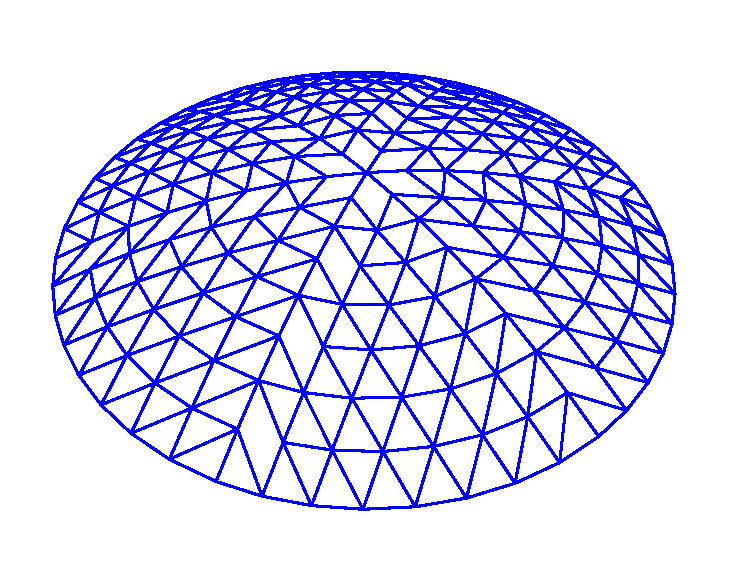
\includegraphics[width=5cm]{images/scallopdome-000}}
    \hfill
    \subfigure[Another Scallopdome]{\label{scallop2}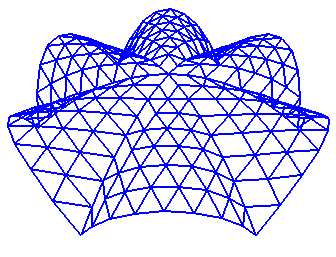
\includegraphics[width=5cm]{images/scallopdome-001}}
    \hfill
    \subfigure[Yet another Scallopdome]{\label{scallop3}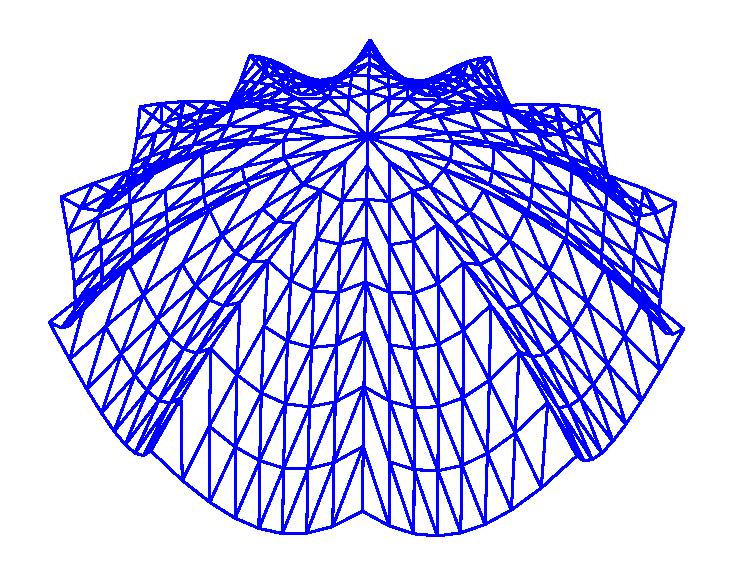
\includegraphics[width=5cm]{images/scallopdome-002}}
  \end{latexonly}
  \begin{htmlonly}
%    \htmladdimg[WIDTH="300"]{images/scallopdome-000.png}
    \htmladdimg{images/scallopdome-000.png}
    \htmladdimg{images/scallopdome-001.png}
    \htmladdimg{images/scallopdome-002.png}
  \end{htmlonly}
  \caption{Same script, different domes} \label{fig:scallops}
\end{figure}

% As mentioned, \pyformex is based on the programming language Python \footnote{\url{http://www.python.org}}. This implies that the scripts are also Python-based. It's a very easy language, but if you're interested in reading more, there is a very good tutorial available on \url{http://docs.python.org/tut/}. However, if you're only using Python to write \pyformex-scripts, the tutorial you're reading right now should be enough. 


%%%%%%%%%%%%%%%%%%%%%%%%%%%%%%%%%%%%%%%%%%%%%%%%%%%%%%%%%%%%%%%%%%%
\section{Getting started}
\label{sec:getting-started}

This section holds some basic information on how to use Python and \pyformex. 

\begin{itemize}
\item Each script should begin with \Code{\#!/usr/bin/env python pyformex.py}
\item To start the \pyformex GUI, double click on the file \file{pyformex} in the installation directory, or type \emph{pyformex} in the terminal. Using the terminal can be very useful, because errors that are created while running the script will appear in the terminal. This can provide useful information when something goes wrong with your script.
\item To create a new \pyformex-script, just open a new file with your favorite text editor and save it as \file{myproject.py}.
\item To edit a script, you can
	\begin{itemize}
	\item Open it with your favorite text editor.
	\item \menuselection{File \sub Open}\\
	At this point, the script will be loaded but nothing will happen. \\
	\menuselection{File \sub Edit}\\
	The script will now open in the default text editor. This default editor can be changed in the user configuration file (\file{~/.pyformexrc}) or using the \menuselection{Settings \sub Commands} menu option.
	\end{itemize}
\item To play a script, you can
	\begin{itemize}
	\item \menuselection{File \sub Open}\\
		\menuselection{File \sub Play} 
	\item Type \emph{pyformex myproject.py} in the terminal. This will start the \pyformex GUI and load your script at the same time. \\
\menuselection{File \sub Play}
	\item To play a script without using the GUI (for example in finite element preprocessing, if you only want to write an 		output file, without drawing the structure), type \emph{pyformex --nogui myproject.py}
	\end{itemize}
\item When writing a script in Python, there are some things you should keep in mind:
	\begin{itemize}
	\item When using a function that requires arguments, an argument list must have any positional arguments followed by any keyword arguments, where the keywords must be chosen from the formal parameter names. It's not important whether a formal parameter has a default value or not. No argument may receive a value more than once -- formal parameter names corresponding to positional arguments cannot be used as keywords in the same calls. 

Simply put: you can either set the arguments in the right order and only give their value, or you can give arguments by their name and value. This last option holds some advantages: not only is it easier to check what you did, but sometimes a function has many arguments with default values and you only want to change a few.
If this isn't entirely clear yet, just look at the examples later in this tutorial or check the Python tutorial.
	\item Indentation is essential in Python. Indentation is Python's way of grouping statements. In straight-forward scripts, indentation is not needed (and forbidden!), but when using a for-statement for example, the body of the statement has to be indented. A small example might make this clear. Also notice the ':' 
\begin{verbatim}
	print 'properties'
	for key, item in properties.iteritems():
	    print key, item
\end{verbatim}
	\item If you want to use functions from a seperate module (like \module{properties}), you add a line on top of the script
\begin{verbatim}
	from properties import *
\end{verbatim}
All functions from that module are now available.
	\item The hash character, "\#", is used to start a comment in Python.
	\item Python is case sensative.
	\end{itemize}
\end{itemize}


%%%%%%%%%%%%%%%%%%%%%%%%%%%%%%%%%%%%%%%%%%%%%%%%%%%%%%%%%%%%%%%%%
\section{The geometrical model}
\label{sec:geom}


\subsection{Creating a Formex}
\label{subsec:create}

\subsubsection{What is a Formex?}
A Formex\index{Formex} is a numarray of order 3 (axes 0,1,2) and type Float.
A scalar element represents a coordinate (F:uniple).

    A row along the axis 2 is a set of coordinates and represents a point
    (node, vertex, F: signet).
    For simplicity's sake, the current implementation only deals with points
    in a 3-dimensional space. This means that the length of axis 2 is always 3.
    The user can create Formices (plural of Formex) in a 2-D space, but
    internally these will be stored with 3 coordinates, by adding a third
    value 0. All operations work with 3-D coordinate sets. However, a method
    exists to extract only a limited set of coordinates from the results,
    permitting to return to a 2-D environment.

    A plane along the axes 2 and 1 is a set of points (F: cantle). This can be
    thought of as a geometrical shape (2 points form a line segment, 3 points
    make a triangle, ...) or as an element in FE terms. But it really is up to
    the user as to how this set of points is to be interpreted.

    Finally, the whole Formex represents a set of such elements.

    Additionally, a Formex may have a property set, which is an 1-D array of
    integers. The length of the array is equal to the length of axis 0 of the
    Formex data (i.e. the number of elements in the Formex). Thus, a single
    integer value may be attributed to each element. It is up to the user to
    define the use of this integer (e.g. it could be an index in a table of
    element property records).
    If a property set is defined, it will be copied together with the Formex
    data whenever copies of the Formex (or parts thereof) are made.
    Properties can be specified at creation time, and they can be set,
    modified or deleted at any time. Of course, the properties that are
    copied in an operation are those that exist at the time of performing
    the operation.   

Simply put: a Formex is a set of elements, and every element can have a property number.
\begin{figure}[ht]
  \centering
  \begin{makeimage}
  \end{makeimage}
  \begin{latexonly}
    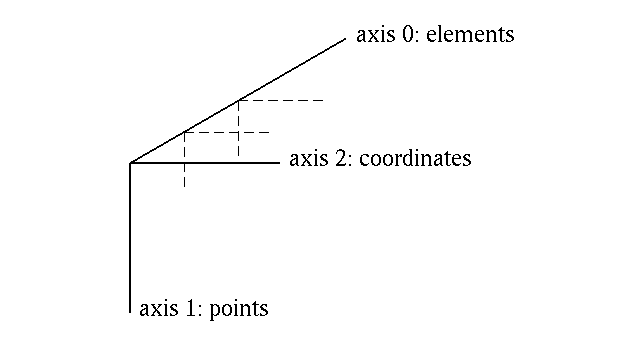
\includegraphics{images/Formex}
  \end{latexonly}
  \begin{htmlonly}
    \htmladdimg{images/Formex.png}
  \end{htmlonly}  
  \caption{The scheme of a Formex}
\end{figure}

\subsubsection{Creating a Formex using coordinates}
The first and most useful way to create a Formex is by specifying it's nodes and elements in a 3D-list.  

\begin{verbatim}
	F=Formex([[[0,0],[1,0],[1,1],[0,1]]])
\end{verbatim}

\begin{figure}[ht]
  \centering
  \begin{makeimage}
  \end{makeimage}
  \begin{latexonly}
    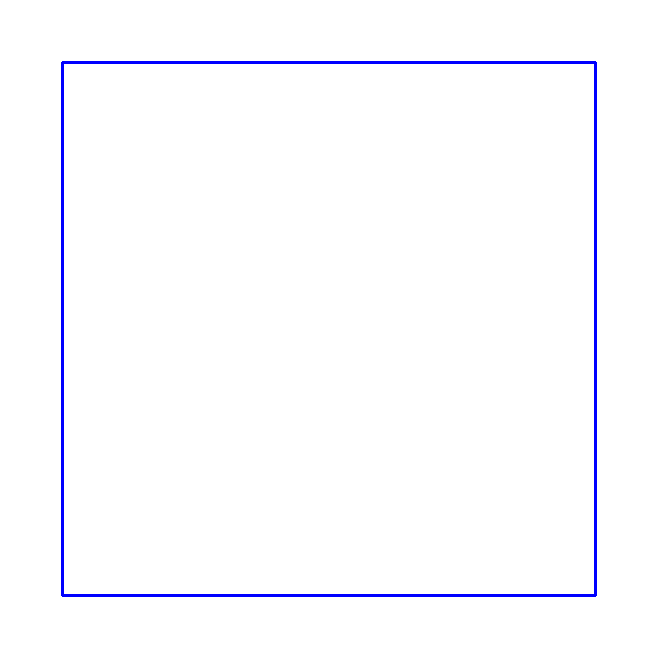
\includegraphics[width=4cm]{images/square}
  \end{latexonly}
  \begin{htmlonly}
    \htmladdimg{images/square.png}
  \end{htmlonly}  
  \caption{A very simple Formex}
  \label{fig:square}
\end{figure}

This creates a Formex F, which has the nodes (0,0), (1,0), (1,1) and (0,1). These nodes are all part of a single element, thus creating a square plane. This element is also the entire Formex.
On the other hand, if you would change the position of the square brackets like in the following example, then you'd create a Formex F which is different from the previous. The nodes are the same, but the connection is different. The nodes (0,0) and (1,0) are linked together by an element, and so are the nodes (1,1) and (0,1). The Formex is now a set of 2 parallel bars, instead of a single square plane. 
\begin{verbatim}
	F=Formex([[[0,0],[1,0]],[[1,1],[0,1]]])
\end{verbatim}

\begin{figure}[ht]
  \centering
  \begin{makeimage}
  \end{makeimage}
  \begin{latexonly}
    
\includegraphics[width=4cm]{images/parallel}
  \end{latexonly}
  \begin{htmlonly}
    \htmladdimg{images/parallel.png}
  \end{htmlonly}  
  \caption{Same nodes, different Formex}
\end{figure}

If we want to define a Formex, similar to the square plane, but consisting of the 4 edges instead of the actual plane, we have to define four elements and combine them in a Formex. This is \emph{not} the same Formex as fig \ref{fig:square}, although it looks exactly the same.
\begin{verbatim}
	F=Formex([[[0,0],[0,1]], [[0,1],[1,1]], [[1,1],[1,0]], [[1,0],[0,0]]])
\end{verbatim}

The previous examples were limited to a 2-D environment for simplicity's sake. Of course, we could add a third dimension. For instance, it's no problem defining a pyramid consisting of 8 elements ('bars').
\begin{verbatim}
	F=Formex([[[0,0,0],[0,1,0]], [[0,1,0],[1,1,0]], [[1,1,0],[1,0,0]], [[1,0,0], 
		[0,0,0]], [[0,0,0],[0,1,0]], [[0,0,0],[0.5,0.5,1]], [[1,0,0],[0.5,0.5,1]], 
		[[1,1,0], [0.5,0.5,1]], [[0,1,0],[0.5,0.5,1]]])
\end{verbatim}

\begin{figure}[ht]
  \centering
  \begin{makeimage}
  \end{makeimage}
  \begin{latexonly}
    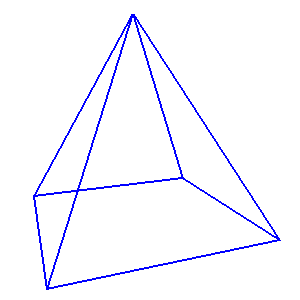
\includegraphics[width=6cm]{images/pyramide}
  \end{latexonly}
  \begin{htmlonly}
    \htmladdimg{images/pyramide.png}
  \end{htmlonly}  
  \caption{A pyramid}
  \label{fig:pyramid}
\end{figure}

However, as you can see, even in this very small example the number of nodes, elements and coordinates you have to declare becomes rather large. Defining large Formices using this method would not be practical. This problem is easily overcome by copying, translating, rotating,... a smaller Formex --- as will be explained in \ref{subsec:changing} --- or by using patterns.
 
\subsubsection{Creating a Formex using patterns}

The second way of creating a new Formex, is by defining patterns. In this case, a line segment pattern is created from a string.

The function \function{pattern(s)} creates a list of line segments where all nodes lie on the
gridpoints of a regular grid with unit step.
The first point of the list is [0,0,0]. Each character from the given
string \var{s} is interpreted as a code specifying how to move to the next node.
Currently defined are the following codes:\\
    0 = goto origin [0,0,0]\\
    1..8 move in the x,y plane\\
    9 remains at the same place\\
    When looking at the plane with the x-axis to the right,\\
    1 = East, 2 = North, 3 = West, 4 = South, 5 = NE, 6 = NW, 7 = SW, 8 = SE.\\
    Adding 16 to the ordinal of the character causes an extra move of +1 in
    the z-direction. Adding 48 causes an extra move of -1. This means that
    'ABCDEFGHI', resp. 'abcdefghi', correspond with '123456789' with an extra
    z +/-= 1.              
    The special character '\verb?\?' can be put before any character to make the
    move without making a connection.
    The effect of any other character is undefined.

This method has important restrictions, since it can only create lines on a regular grid. However, it can be a much easier and shorter way to define a simple Formex. This is illustrated by the difference in length between the previous creation of a square and the next one, although they define the same Formex (figure \ref{fig:square}).
\begin{verbatim}
	F=Formex(pattern('1234'))
\end{verbatim}

Some simple patterns are defined in \module{simple.py} and are ready for use. These patterns are stacked in a dictionary called 'Patterns'. Items of this dictionary can be accessed like \Code{Patterns['cube']}.
\begin{verbatim}
	#!/usr/bin/env pyformex
	from simple import *
	c=Formex(pattern(Pattern['cube']))
	clear();draw(c)
\end{verbatim}

\begin{figure}[ht]
  \centering
  \begin{makeimage}
  \end{makeimage}
  \begin{latexonly}
    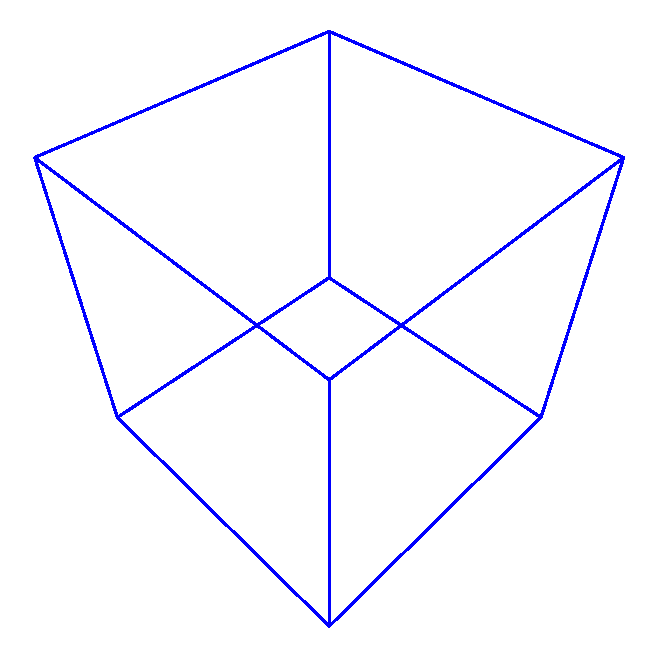
\includegraphics[width=6cm]{images/cube}
  \end{latexonly}
  \begin{htmlonly}
    \htmladdimg{images/cube.png}
  \end{htmlonly}  
  \caption{A cube}
  \label{fig:cube}
\end{figure}

\subsubsection{Creating a Formex using coordinates from a file}
In some cases, you might want to read coordinates from a file an combine them into a Formex. This is possible with the module \module{file2formex} and it's function \function{fileFormex()}. Each point is connected to the following, forming an element (bar).

The next file ('square.txt') would create the same square as before(figure \ref{fig:square}).
\begin{verbatim}
	0,0,0
	0,1,0
	1,1,0
	1,0,0
\end{verbatim}
\begin{verbatim}
	#!/usr/bin/env pyformex
	from file2formex import *
	F=fileFormex('square.text', closed='yes')
\end{verbatim}

\subsection{Adding property numbers}
\label{subsec:propnr}
Each Formex element can have a property number. Each property number is represented by a different color when the Formex is drawn. This is the first reason why you could use property numbers: to make your drawing more transparent or just more beautiful. However, these numbers can also be used as an entry in a dictionary of properties - thus linking the element with a property. This property can be about anything, but in finite element processing this would be the element section, material, loads,... The use of properties in this way will be futher explained in \ref{sec:props}.
Property numbers can be specified at creation time, and they can be set, modified or deleted at any time.  
\begin{verbatim}
>>> #!/usr/bin/env pyformex
>>> F=Formex(pattern('1234'),[5])
>>> print F.prop()
>>> G=Formex(pattern('1234'),[6,8,2,4])
>>> print G.prop()
>>> F.setProp([6,7])
>>> print F.prop()
>>> G.setProp([6,7,8,9])
>>> print G.prop()

[5 5 5 5]
[6 8 2 4]
[6 7 6 7]
[6 7 8 9]
\end{verbatim}

\subsection{Drawing a Formex}
\label{subsec:drawing}
Of course, you'd want to see what you have created. This is accomplished by the function \function{draw()}. The next example creates figure \ref{fig:pyramid}. 
\begin{verbatim}
	F=Formex([[[0,0,0],[0,1,0]], [[0,1,0],[1,1,0]], [[1,1,0],[1,0,0]], [[1,0,0], 
		[0,0,0]], [[0,0,0],[0,1,0]], [[0,0,0],[0.5,0.5,1]], [[1,0,0],[0.5,0.5,1]], 
		[[1,1,0], [0.5,0.5,1]], [[0,1,0],[0.5,0.5,1]]])
	draw(F)
\end{verbatim}

It also possible to draw multiple Formices at the same time.
\begin{verbatim}
	from simple import *
	F=Formex([[[0,0,0],[0,1,0]], [[0,1,0],[1,1,0]], [[1,1,0],[1,0,0]], [[1,0,0],
		[0,0,0]], [[0,0,0],[0,1,0]], [[0,0,0],[0.5,0.5,1]], [[1,0,0],[0.5,0.5,1]], 
		[[1,1,0],[0.5,0.5,1]], [[0,1,0],[0.5,0.5,1]]]).setProp(1)	
	G=Formex(pattern(Pattern['cube'])).setProp(3)
	draw(F+G)
\end{verbatim}
\begin{figure}[ht]
  \centering
  \begin{makeimage}
  \end{makeimage}
  \begin{latexonly}
    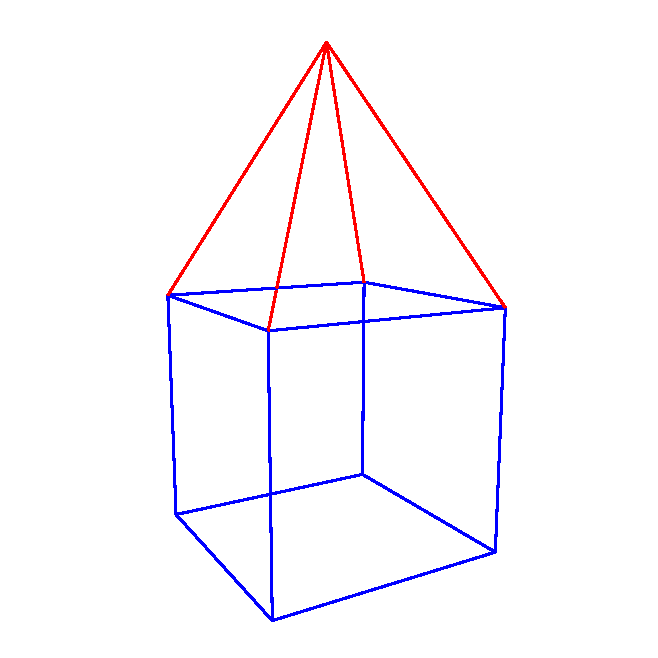
\includegraphics[width=6cm]{images/house}
  \end{latexonly}
  \begin{htmlonly}
    \htmladdimg{images/house.png}
  \end{htmlonly}  
  \caption{Drawing multiple Formices}
  \label{fig:multiple}
\end{figure}
 
It might be important to realize that even if you don't draw a particular Formex, that doesn't mean you didn't create it!

Now, when you are creating a large geometry, you might be interested in seeing the different steps in the creation. To remove all previously drawn Formices, you can use \function{clear()}  what sweepes the screen clean. If you want to see a certain step in the creation longer than the default time, use \function{sleep(t)}, with \var{t} the delay (in seconds) before executing the next command.
\begin{verbatim}
	F=Formex(pattern('164'))
	draw(F)
	G=F.replic(5,1,0)
	clear()
	draw(G)
\end{verbatim}


\subsection{Saving images}
\label{subsec:images}
After drawing the Formex, you might want to save the image. This is very easy to do:\\
\menuselection{File \sub Save Image}\\
The filetype should be 'bmp', 'jpg', 'pbm', 'png', 'ppm', 'xbm', 'xpm', 'eps', 'ps', 'pdf' or 'tex'. \\
To create a better looking picture, several settings can be changed:
\begin{itemize}
	\item Change the background color \menuselection{Settings \sub Background Color}
	\item Use a different (bigger) linewidth \menuselection{Settings \sub Linewidth}
	\item Change the canvas size. This prevents having to cut and rescale the figure with an image manipulation program (and loosing quality by doing so).  \menuselection{Settings \sub Canvas Size}
\end{itemize}

It is also possible to save a series of images. This can be especially useful when playing a script which creates several images, and you would like to save them all.  For example, figure \ref{fig:WireStent-steps}, which shows the different steps in the creation of the WireStent model, was created this way.\\
\menuselection{File \sub Toggle MultiSave}\\


\subsection{Information about a Formex}
\label{subsec:info}
There are a number of functions available that return information about a Formex. Especially when using \pyformex as finite element preprocessor, the most useful functions are:
\begin{tableii}{l|l}{exception}{Function}{Description}
	\lineii{F.nelems()			}
		{Return the number of elements in the Formex.}
	\lineii{F.nnodes() 			}
		{Return the number of nodes in the Formex.}
	\lineii{F.prop() 				}
		{Return the properties as a numpy array.}
	\lineii{F.bbox()				}
		{Return the bounding box of the Formex.}
	\lineii{F.center()			}
		{Return the center of the Formex.}
	\lineii{F.feModel()	}
		{Return a tuple of nodal coordinates and element connectivity.}
\end{tableii}

\function{feModel()} is very important in finite element processing. It returns all nodes and all elements of the Formex in a format useful for FE processing. A tuple of two arrays is returned. The first is float array with the coordinates of the unique nodes of the Formex. The second is an integer array with the node numbers connected by each element.
\begin{verbatim}
>>> #!/usr/bin/env pyformex
>>> from simple import *

>>> c = Formex(pattern(Pattern['cube']))
>>> draw(c)
>>> nodes,elems = c.feModel()
>>> print 'Nodes'
>>> print nodes
>>> print 'Elements'
>>> print elems

Nodes
[[ 0.  0. -1.]
 [ 1.  0. -1.]
 [ 0.  1. -1.]
 [ 1.  1. -1.]
 [ 0.  0.  0.]
 [ 1.  0.  0.]
 [ 0.  1.  0.]
 [ 1.  1.  0.]]
Elements
[[4 5]
 [5 7]
 [7 6]
 [6 4]
 [4 0]
 [5 1]
 [7 3]
 [6 2]
 [0 1]
 [1 3]
 [3 2]
 [2 0]]
\end{verbatim}

\subsection{Changing the Formex}
\label{subsec:changing}
Until now, we've only created simple Formices. The strength of \pyformex however is that it is very easy to generate large geometrical models by a sequence of mathematical transformations. After initiating a basic Formex, it's possible to transform it by using copies, translations, rotations, projections,...

There are many transformations available, but this is not the right place to describe them all. This is what the reference manual in chapter \ref{cha:reference} is for. A summary of all possible transformations and functions can be found there.

To illustrate some of these transformations and the recommended way of writing a script, we will analyse some of the examples. More of these interesting examples are found in \file{installdir/examples}. Let's begin with the example \file{Spiral.py}. 

\verbatiminput{scripts/Spiral.py}

During this first read-through, you will have noticed that every step is drawn. Of course, this is not necessary, but it can be useful. And above all, it is very educational for use in a tutorial...

The next important thing is that parameters were used. It's recommended to always do this, especially when you want to do a parametric study of course, but it can also be very convenient if at some point you want to change the geometry (for example when you want to re-use the script for another application).

A simple function \function{drawit()} is defined for use in this script only. This function only provides a shorter way of drawing Formices, since it combines \function{clear()} and \function{draw}. 

Now, let's dissect the script.

\begin{verbatim}
def drawit(F,view='front'):
    clear()
    draw(F,view)
\end{verbatim}
This is a small function that is only defined in this script. It clears the screen and draws the Formex at the same time. 

\begin{verbatim}
m = 36 # number of cells along torus big circle
n = 10 # number of cells along torus small circle
\end{verbatim}
These are the parameters. They can easily be changed, and a whole new spiral will be created without any extra effort.
The first step is to create a basic Formex. In this case, it's a triangle which has a different property number for every edge.
\begin{verbatim}
F = Formex(pattern("164"),[1,2,3]); drawit(F)  
\end{verbatim}
\begin{figure}[ht]
  \centering
  \begin{makeimage}
  \end{makeimage}
  \begin{latexonly}
    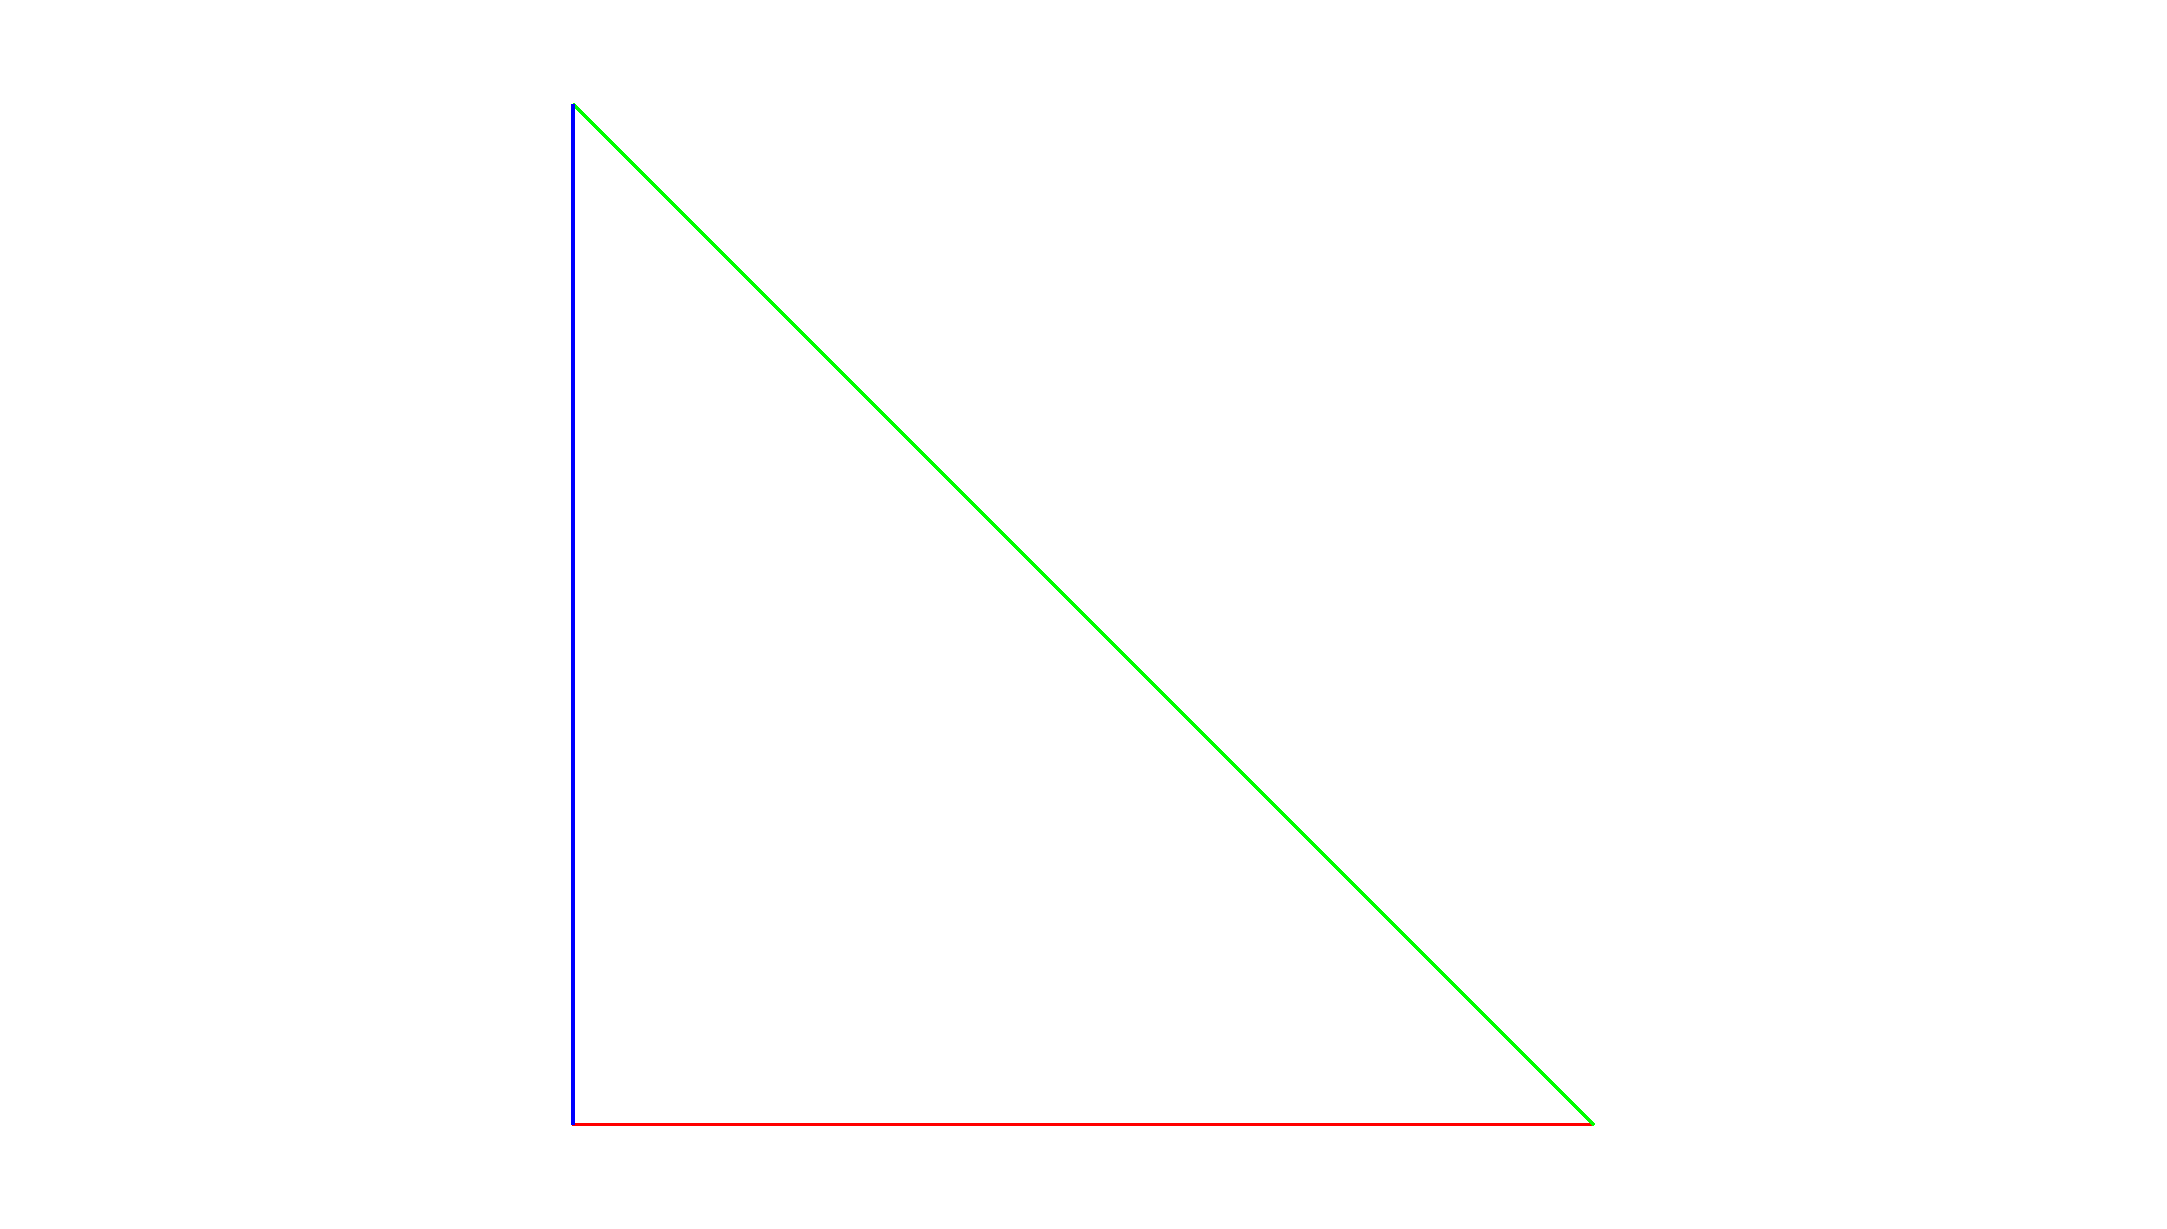
\includegraphics[width=6cm]{images/spiral-000}
  \end{latexonly}
  \begin{htmlonly}
    \htmladdimg{images/spiral-000.png}
  \end{htmlonly}  
  \caption{The basic Formex}
\end{figure}

This basic Formex is copied 'm' times in the 0-direction with a translation 
step of '1' (the length of an edge of the triangle). After that, the new 
Formex is copied 'n' times in the 1-direction with a translation step of '1'. 
Because of the recursive definition (F=F.replic), the original Formex F is 
overwritten by the transformed one.
\begin{verbatim}
F = F.replic(m,1,0); drawit(F)
F = F.replic(n,1,1); drawit(F)
\end{verbatim}

Now a copy of this last Formex is translated in direction '2' with a 
translation step of '1'. This necessary for the transformation into a cilinder.
The result of all previous steps is a rectangular pattern with the desired 
dimensions, in a plane z=1.
\begin{verbatim}
F = F.translate(2,1); drawit(F,'iso')
\end{verbatim}
\begin{figure}[ht]
  \centering
  \begin{makeimage}
  \end{makeimage}
  \begin{latexonly}
    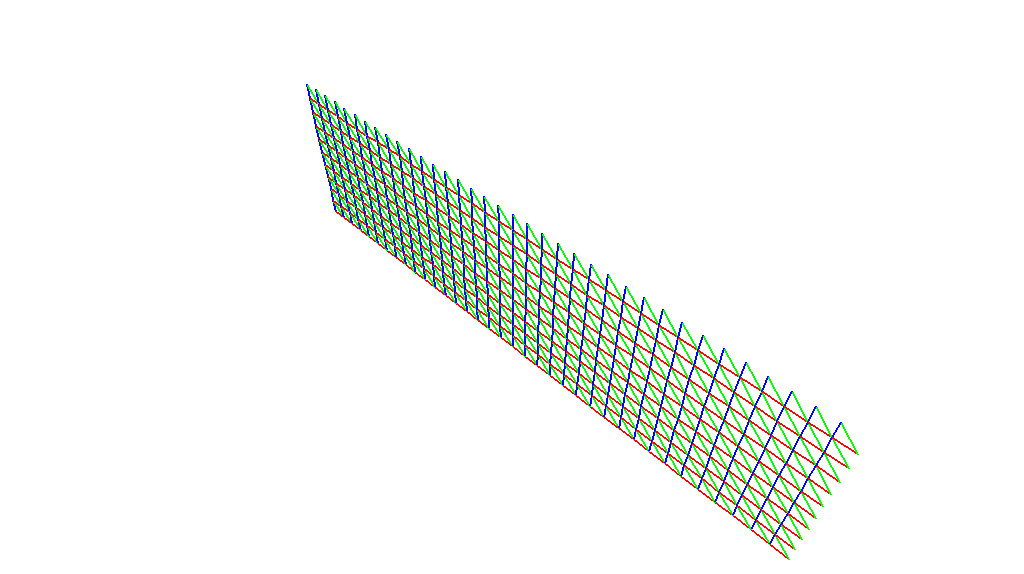
\includegraphics[width=6cm]{images/spiral-003}
  \end{latexonly}
  \begin{htmlonly}
    \htmladdimg{images/spiral-003.png}
  \end{htmlonly}  
  \caption{The rectangular pattern}
\end{figure}

This pattern is rolled up into a cilinder around the 2-axis. 
\begin{verbatim}
F = F.cylindrical([2,1,0],[1.,360./n,1.]); drawit(F,'iso')
\end{verbatim}
\begin{figure}[ht]
  \centering
  \begin{makeimage}
  \end{makeimage}
  \begin{latexonly}
    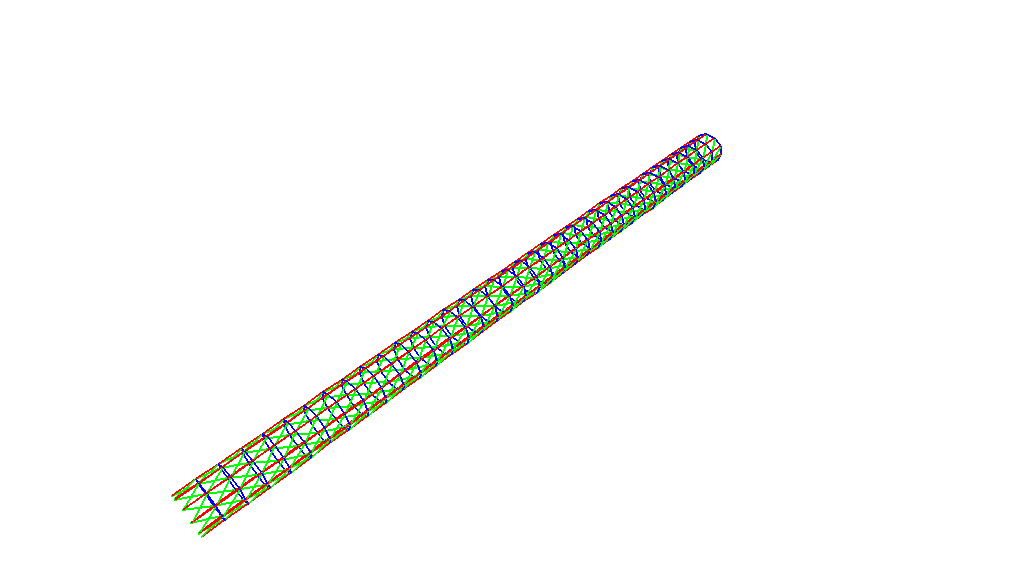
\includegraphics[width=6cm]{images/spiral-004}
  \end{latexonly}
  \begin{htmlonly}
    \htmladdimg{images/spiral-004.png}
  \end{htmlonly}  
  \caption{The cylinder}
\end{figure}

This cilinder is copied 5 times in the 2-direction with a translation step of 
'm' (the lenght of the cilinder). 
\begin{verbatim}
F = F.replic(5,m,2); drawit(F,'iso')
\end{verbatim}

The next step is to rotate this cilinder -10 degrees around the 0-axis. 
This will determine the pitch angle of the spiral.
\begin{verbatim}
F = F.rotate(-10,0); drawit(F,'iso')
\end{verbatim}
\begin{figure}[ht]
  \centering
  \begin{makeimage}
  \end{makeimage}
  \begin{latexonly}
    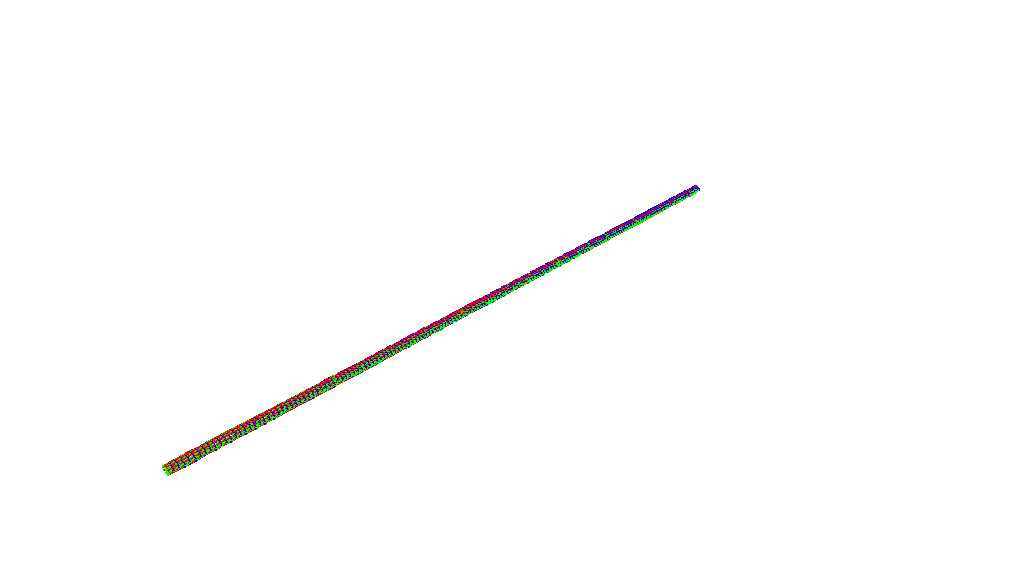
\includegraphics[width=6cm]{images/spiral-006}
  \end{latexonly}
  \begin{htmlonly}
    \htmladdimg{images/spiral-006.png}
  \end{htmlonly}  
  \caption{The new cylinder}
\end{figure}

This last Formex is now translated in direction '0' with a translation step of '5'. 
\begin{verbatim}
F = F.translate(0,5); drawit(F,'iso')
\end{verbatim}

Finally, the Formex is rolled up, but around a different axis then before. 
Due to the pitch angle, a spiral is created. If the pitch angle would be 0 
(no rotation of -10 degrees around the 0-axis), the resulting Formex 
would be a torus. 
\begin{verbatim}
F = F.cylindrical([0,2,1],[1.,360./m,1.]); drawit(F,'iso')
drawit(F,'right')
\end{verbatim}
 \begin{figure}[ht]
   \centering
   \begin{makeimage}
   \end{makeimage}
   \begin{latexonly}
     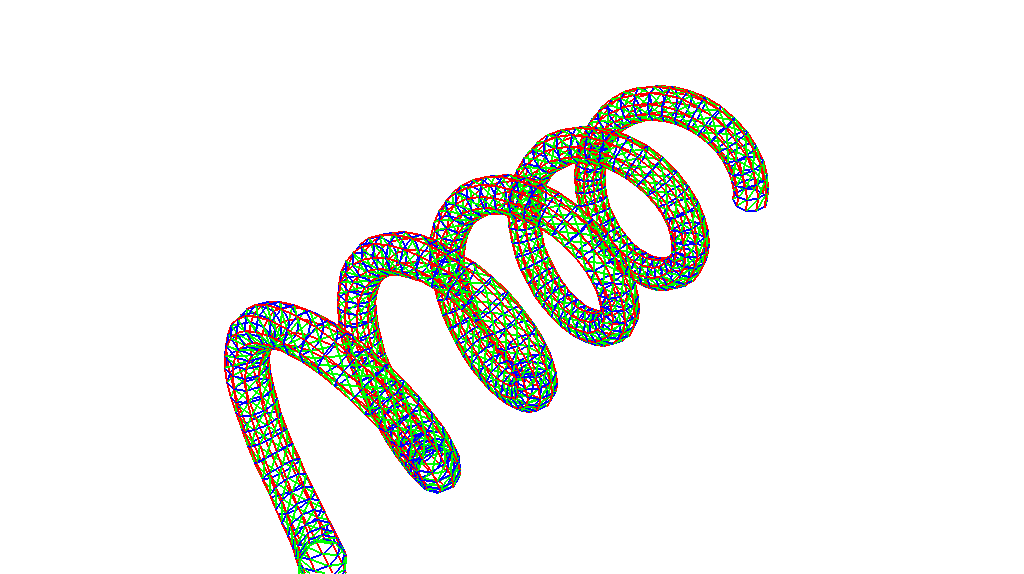
\includegraphics[width=5cm]{images/spiral-007}
     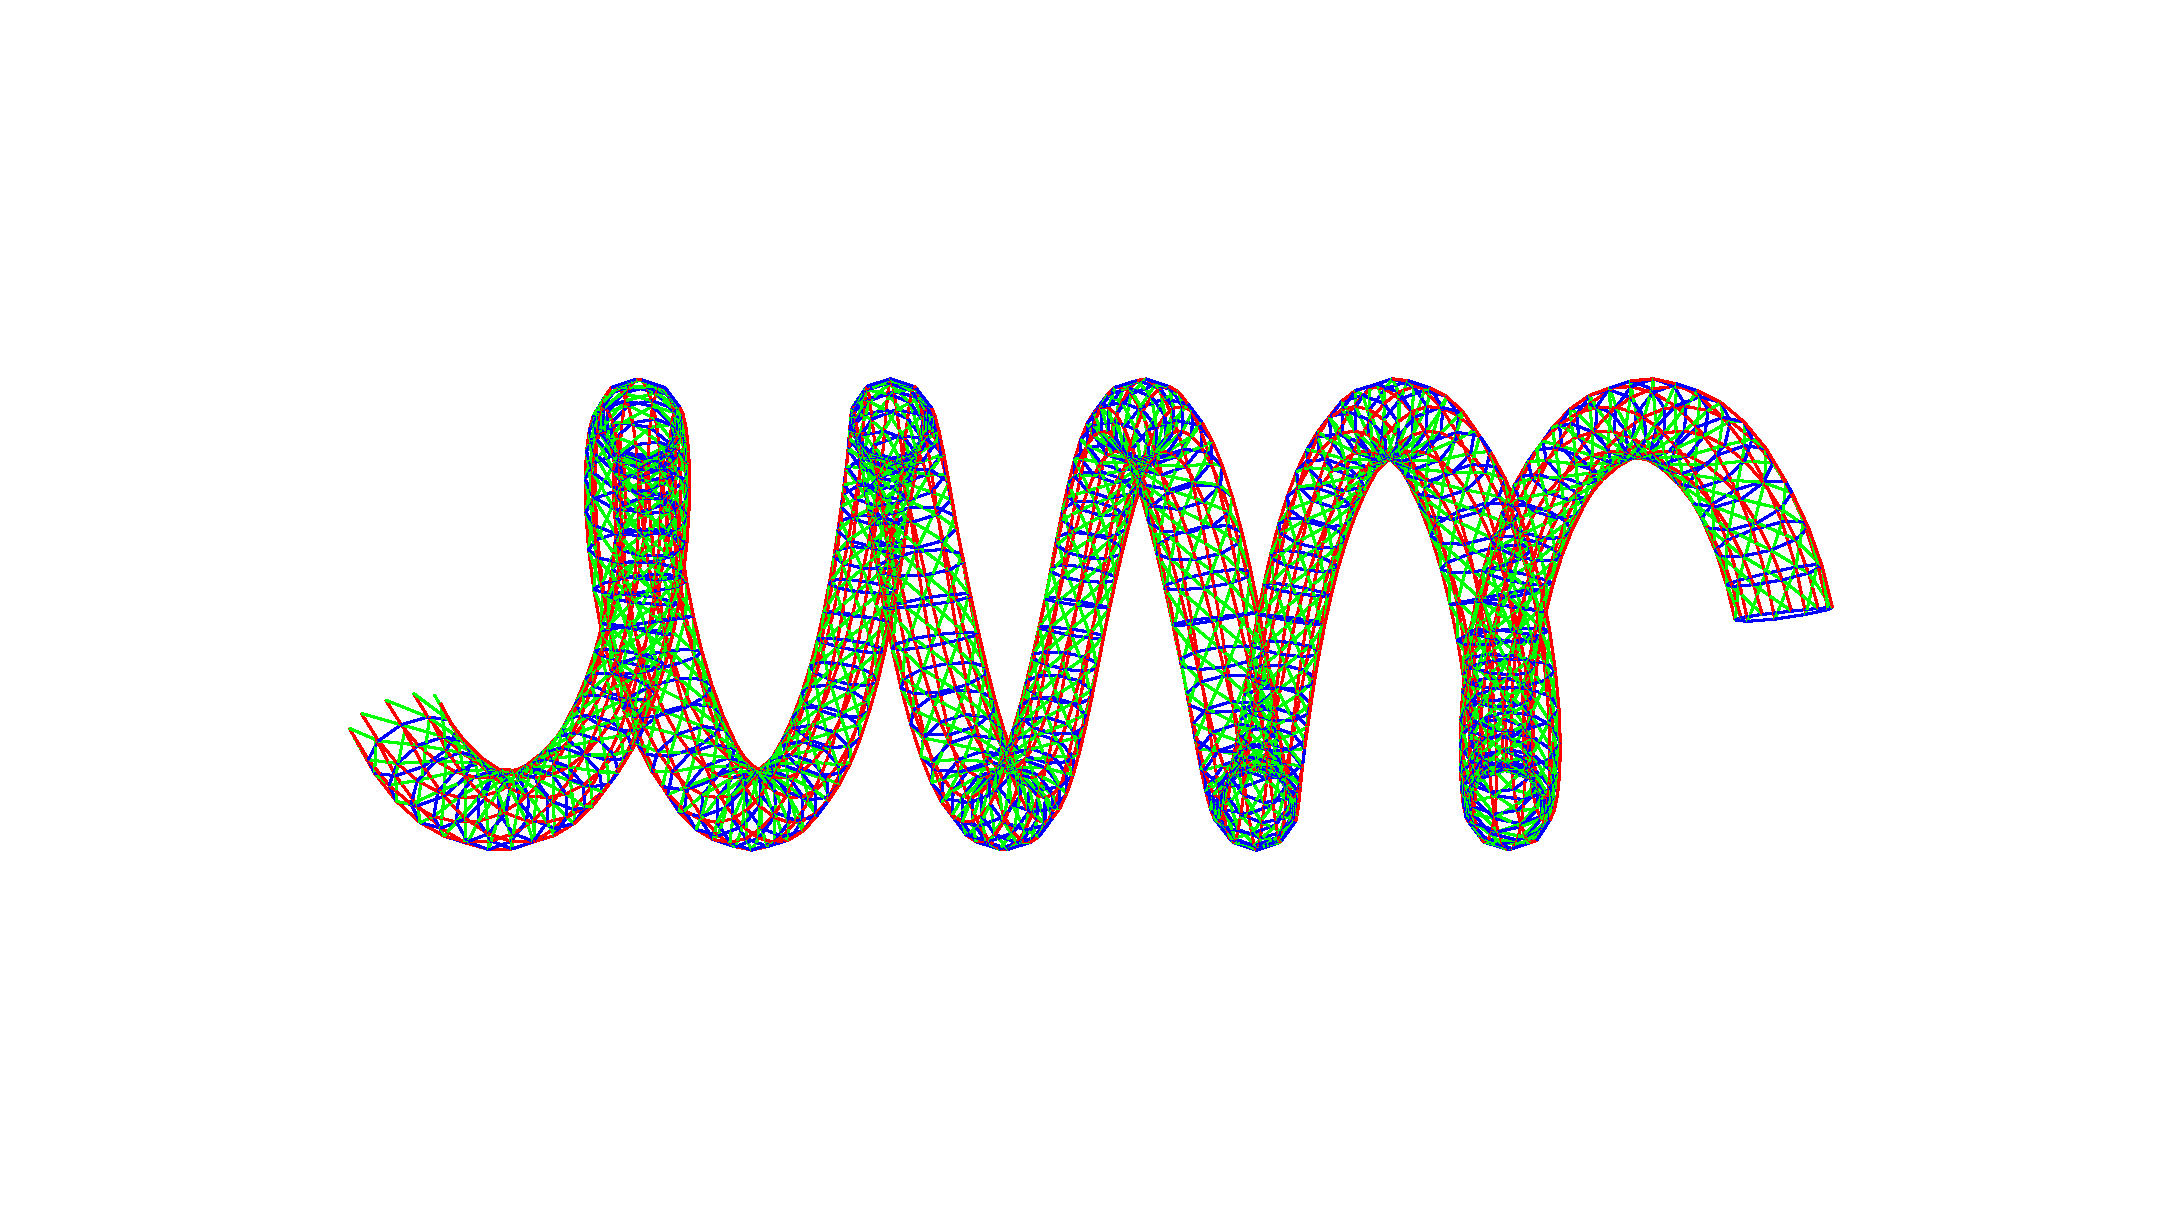
\includegraphics[width=5cm]{images/spiral-008}
   \end{latexonly}
   \begin{htmlonly}
     \htmladdimg{images/spiral-007.png}
     \htmladdimg{images/spiral-008.png}
   \end{htmlonly}  
   \caption{The spiral}
 \end{figure}

%%%%%%%%%%%%%%%%%%%%%%%%%%%%%%%%%%%%%%%%%%%%%%%%%%%%%%%%%%%%%%%%%
\section{Adding properties}
\label{sec:props}
Each element of a Formex can hold a property number. This number can be used as an entry in a database, which holds some sort of property. The module \module{properties} delivers such databases. The Formex and the database are seperate entities, only linked by the property numbers. 

\subsection{The class Property}
The first kind of database is called \class{Property}. This is the base class, and can hold any kind of property.
\begin{verbatim}
>>> Stick = Property(1, {'colour':'green', 'name':'Stick', 'weight': 25, 
'comment':'This could be anything: a gum, a frog, a usb-stick,...'})
>>> author = Property(5,{'Name':'Tim Neels', 'Address': CascadingDict
{'street':'Krijgslaan','city':'Gent','country':'Belgium'})})
\end{verbatim}
Data can be accessed in two ways: through the Property-instance itself, or through a dict 'properties'. 
\begin{verbatim}    
>>> print Stick
>>> print properties[1] 

  comment = This could be anything: a gum, a frog, a usb-stick,...
  colour = green
  name = Stick
  weight = 25

  comment = This could be anything: a gum, a frog, a usb-stick,...
  colour = green
  name = Stick
  weight = 25
\end{verbatim}
Adding and changing properties is very easy.
\begin{verbatim}  
>>> Stick.weight=30
>>> Stick.length=10
>>> print properties[1]

  comment = This could be anything: a gum, a frog, a usb-stick,...
  length = 10
  colour = green
  name = Stick
  weight = 30
\end{verbatim}

\subsection{The class NodeProperty}
The class NodeProperty can hold properties of nodes in finite element processing. The data is stored in a Dict called 'nodeproperties'. A NodeProperty can hold following sub-properties:
 \begin{description}
 \item [cload] A concentrated load. This is a list of 6 items
 \Code{[F_0, F_1, F_2, M_0, M_1, M_2]}. 
 \item [bound] A boundary condition. This can be defined in 2 ways:
     \begin{itemize}
     \item as a list of 6 items \Code{[ R_0, R_1, R_2, M_0, M_1, M_2 ]}. These items have 2 possible values:
         \begin{description}
         \item [0] The degree of freedom is not restrained.
         \item [1] The degree of freedom is restrained.
         \end{description}
     \item as a string. This string is a standard boundary type. In Abaqus several types are available:
         \begin{itemize}
         \item PINNED 
         \item ENCASTRE
         \item XSYMM
         \item YSYMM
         \item ZSYMM
         \item XASYMM
         \item YASYMM 
         \item ZASYMM
         \end{itemize} 
     \end{itemize}
 \item [displacement] The prescribed displacement. 
 \item [coords] The coordinate system which is used for the definition of cload and bound. There are three options:
         cartesian, spherical and cylindrical.
 \item [coordset] A list of 6 coordinates of the 2 points that specify the transformation: \Code{[x_1, y_1, z_1, x_2, y_2, z_2]}.
\end{description}

\begin{verbatim}
>>> top = NodeProperty(1,cload=[5,0,-75,0,0,0])
>>> foot = NodeProperty(2,bound='pinned')
>>> print 'nodeproperties'    
>>> for key, item in nodeproperties.iteritems():
>>>     print key, item

nodeproperties
1
  cload = [5, 0, -75, 0, 0, 0]
  coords = cartesian
  displacement = None
  bound = None
  coordset = []
2
  cload = None
  coords = cartesian
  displacement = None
  bound = pinned
  coordset = []
\end{verbatim}

\subsection{The class ElemProperty}
The class ElemProperty holds properties related to a single element. The data is stored in a Dict called 'elemproperties'. An element property can hold the following sub-properties:
\begin{description}
\item [elemsection] The section properties of the element. This is an ElemSection instance.
\item [elemload] The loading of the element. This is a list of ElemLoad instances.
\item [elemtype] The type of element that is to be used in the analysis. 
\end{description}

An elemsection can hold the following sub-properties:
\begin{description}
\item [section] The section properties of the element. This can be a dictionary or a string. The required data in this dict depends on the sectiontype. 
\item [material] The element material properties. This can be a dictionary which holds these properties or a string which can be used to search a material database. 
\item [sectiontype] The sectiontype of the element. 
\item [orientation]  A list [First direction cosine, second direction cosine, third direction cosine] of the first beam section axis. This allows to change the orientation of the cross-section.
\end{description}

An element load can hold the following sub-properties:
\begin{description}
\item [magnitude] The magnitude of the distibuted load.
\item [loadlabel] The distributed load type label.
\end{description}

The general structure of the element properties database looks like this:
\begin{itemize}
\item[-] Property
\item[-] NodeProperty
    \begin{itemize}
    \item[-] cload
    \item[-] bound
    \item[-] displacement
    \item[-] coords
    \item[-] coordset
    \end{itemize}
\item[-] ElemProperty 
    \begin{itemize}
    \item[-] elemsection
        \begin{itemize}
        \item[-] section
        \item[-] material
        \item[-] sectiontype
        \item[-] orientation
        \end{itemize}
    \item[-] elemload
        \begin{itemize}
        \item[-] magnitude
        \item[-] loadlabel
        \end{itemize}
    \item[-] elemtype
    \end{itemize}
\end{itemize}

\begin{verbatim}
>>> vert = ElemSection('IPEA100', 'steel')
>>> hor = ElemSection({'name':'IPEM800','A':951247,'I':CascadingDict(
{'Ix':1542,'Iy':6251,'Ixy':352})}, {'name':'S400','E':210,'fy':400})
>>> q = ElemLoad(magnitude=2.5, loadlabel='PZ')
>>> top = ElemProperty(1,hor,[q],'B22')
>>> column = ElemProperty(2,vert, elemtype='B22')
>>> diagonal = ElemProperty(4,hor,elemtype='B22')

>>> print 'elemproperties'
>>> for key, item in elemproperties.iteritems():
>>>     print key, item    

elemproperties
1
  elemtype = B22
  elemload = [CascadingDict({'magnitude': 2.5, 'loadlabel': 'PZ'})]
  elemsection =
    section =
      A = 951247
      I =
        Iy = 6251
        Ix = 1542
        Ixy = 352
      name = IPEM800
    material =
      fy = 400
      E = 210
      name = S400
    orientation = None
    sectiontype = general
2
  elemtype = B22
  elemload = None
  elemsection =
    section =
      torsional_rigidity = 1542
      name = IPEA100
      moment_inertia_22 = 1140000
      cross_section = 878
      moment_inertia_11 = 1412000
      moment_inertia_12 = 1254
    material =
      shear_modulus = 25
      young_modulus = 210
      name = steel
    orientation = None
    sectiontype = general
4
  elemtype = B22
  elemload = None
  elemsection =
    section =
      A = 951247
      I =
        Iy = 6251
        Ix = 1542
        Ixy = 352
      name = IPEM800
    material =
      fy = 400
      E = 210
      name = S400
    orientation = None
    sectiontype = general
\end{verbatim}


%
\section{Exporting to finite element programs}


%
%%% Local Variables: 
%%% mode: latex
%%% TeX-master: "pyformex"
%%% End: 

% pyformex manual --- canvas
% $Id$
% (C) B.Verhegghe

\chapter{The Canvas}
\label{cha:canvas}

\section{Introduction}
When you have create a nice and powerful script to generate a 3D structure, you will most likely want to visually inspect that you have indeed created that what you intended. Usually you even will want or need to see intermediate results before you can continue your development. 
For this purpose the \pyformex GUI offers a canvas where structures can be drawn by functions called from a script and interactively be manipulated by menus options and toolbar buttons.

The 3D drawing and rendering functionality is based on OpenGL. Therefore you will need to have OpenGL available on your machine, either in hardware or software. Hardware accelerated OpenGL will of course speed up and ease operations.

The drawing canvas of \pyformex actually is not a single canvas, but can be split up into one to four viewports, which can each individually be used for your drawing purposes. See the viewport menu of the GUI for details about using multiple viewports. In the remainder of this section we will treat the canvas as if it was a single viewport.

\pyformex distinguishes three types of items that can be drawn on the canvas: actors, marks and decorations. The most important class are the actors: these are 3D geometrical structures defined in the global world coordinates. The 3D scene formed by the actors is viewed by a camera from a certain position, with a certain orientation and lens. The result as viewed by the camera is shown on the canvas. The \pyformex scripting language and the GUI provide ample means to move the camera and change the lens settings, allowing translation, rotation, zooming, changing perspective. All the user needs to do to get an actor displayed with the current camera settings, is to add that actor to the scene. There are different types of actors available, but the most important is the FormexActor: a graphical representation of a Formex. It is so important that there is a special function with lots of options to create a FormexActor and add it to the OpenGL scene.
This function, \Code{draw()}, will be explained in detail in the next section.

The second type of canvas items, marks, differ from the actors in that only their position in world coordinates is fixed, but not their orientation. Marks are always drawn in the same way, irrespective of the camera settings. The observer will always have the same view of the item, though it can (and will) move over the canvas when the camera is changed. Marks are primarily used to attach fixed attributes to certain points of the actors, e.g. a big dot, or a text dispaying some identification of the point.

Finally, \pyformex offers decorations, which are items drawn in 2D viewport coordinates and unchangeably attached to the viewport. This can e.g. be used to display text or color legends on the view.

   
\section{Drawing a Formex}
The most important action performed on the canvas is the drawing of a Formex.
This is accomplished with the \Code{draw()} function. If you look at the reference page of this function~\ref{sec:drawing}, the number of arguments looks frightening. However, most of these arguments have sensible default values, making the access to drawing functionality easy even for beginners. To display your created Formex \Code{F} on the screen, a simple \Code{draw(F)} will suffice in many cases.

If you draw several Formices with subsequent \Code{draw()} commands, they will clutter the view. You can use the \Code{clear()} instruction to wipe out the screen before drawing the next one. If you want to see them together in the same view, you can use different colors to differentiate. Color drawing is as easy as \Code{draw(F,color='red')}. The color specification can take various forms. It can be a single color or an array of colors or even an array of indices in a color table. In the latter case you use \Code{draw(F,color=indices,colormap=table)} to draw the Formex. If multiple colors are specified, each elementof the Formex will be drawn with the corresponding color, and if the color array (or the color indices array) has less entries than the number of elements, it is wrapped around.

A single color entry can be specified by a string ('red') or by a triple of RGB values in the range 0.0..1.0 (e.g. red is (1.0,0.0,0.0)) or a triplet of integer values in the range 0..255 or a hexadecimal string ('\#FF0000') or generally any of the values that can be converted by the colors.glColor() function to a triplet of RGB values.

If no color is specified and your Formex has no properties, \pyformex will draw it with the current drawing color. If the Formex has properties, \pyformex will use the properies as a color index into the specified color map or a (configurable) default color map.

\Todo{There should be some examples here.}


 
\section{Viewing the scene}
Once the Formex is drawn, you can manipulate it interactively using the mouse: you can rotate, translate and zoom with any of the methods decribed in \ref{cha:gui}. You should understand though that these methods do not change your Formex, but only how it is viewed by the observer. 

Our drawing board is based on OpenGL. The whole OpenGL drawing/viewing process can best be understood by making the comparison with the set of a movie, in which actors appear in a 3D scene, and a camera that creates a 2D image by looking at the scene with a certain lens from some angle and distance. Drawing a Formex then is nothing more than making an actor appear on the scene. The OpenGL machine will render it according to the current camera settings. 

Viewing transformations using the mouse will only affect the camera, but not the scene. Thus, if you move the Formex by sliding your mouse with button 3 depressed to the right, the Formex will \emph{look like it is moving to the right,} though it is actually not: we simply move the camera in the opposite direction. Therefore, you will notice that moving the scene will not just translation the picture: its shape will change too, because of changing perspective.

This also explains why there are two ways of zooming: either by changing the focal length of the lens (lens zooming) or by moving the camera towards or away from the scene (dolly zooming). The first one will change the perspective view of the scene, while the second one will not. 

The easiest way to set all camera parameters for properly viewing a scene is by justing telling the direction from which you want to look, and let the program determine the rest of the settings itself. \pyformex even goes a step further and has a number of built in directions readily available: 'top', 'bottom', 'left', 'right', 'front', 'back' will set up the camera looking from that direction.

\section{Other canvas items}


\subsection{Actors}

\subsection{Marks}

\subsection{Decorations}
  


%%% Local Variables: 
%%% mode: latex
%%% TeX-master: "manual"
%%% End: 

% pyformex manual --- gui
% $Id$
% (C) B.Verhegghe

\chapter{The Graphical User Interface}
\label{cha:gui}

\section{Starting the GUI}
You start the \pyf GUI by entering the command \Code{pyformex --gui}. Depending on your installation, you may also have a panel or menu button on your desktop from which you can start the \pyf graphical interface by a simple mouse click. 
%Finally, you can start the GUI with the command \Code{startGUI()} in a \pyf script.

When the main window appears, it will look like the one shown in the figure~\ref{fig:gui}. Your window manager will most likely have put some decorations around it, but these are very much OS and window manager dependent and are therefore not shown in the figure.

\begin{figure}[ht]
  \centering
  \begin{makeimage}
  \end{makeimage}
  \begin{latexonly}
    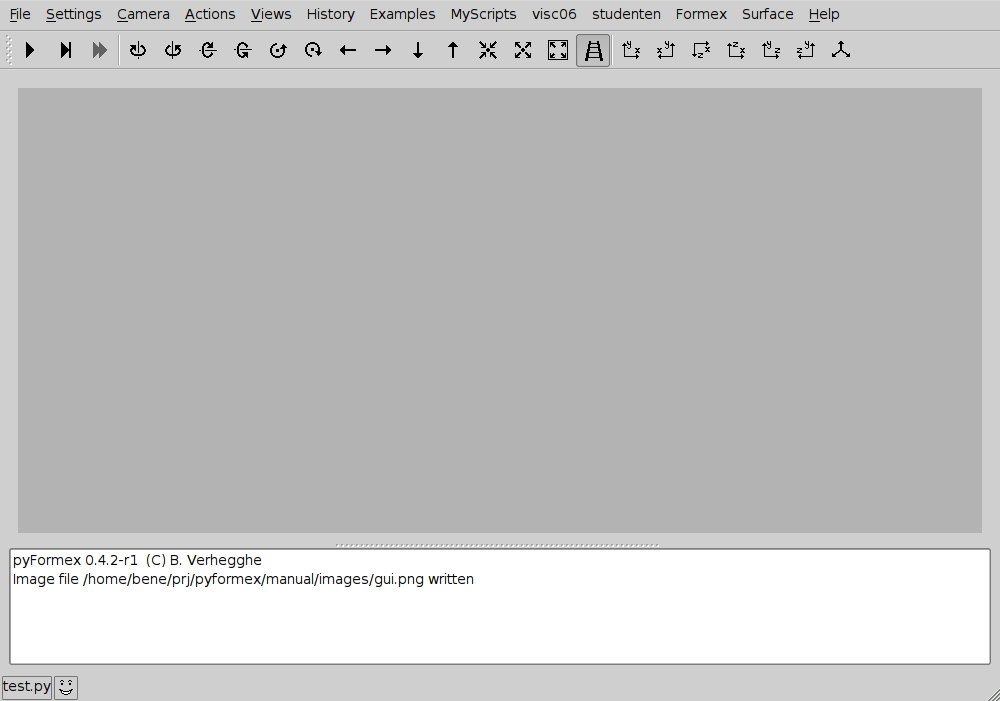
\includegraphics[width=10cm]{images/gui}
  \end{latexonly}
  \begin{htmlonly}
    \htmladdimg{images/gui.png}
  \end{htmlonly}  
  \caption{The pyFormex main window}
  \label{fig:gui}
\end{figure}

\section{Basic use of the GUI}

As \pyf is still in its infancy, the GUI is subject to frequent changes and it would make no sense to cover here every single aspect of it. Rather we will describe the most important functions, so that users can quickly get used to working with \pyf. Also we will present some of the more obscure features that users may not expect but yet might be very useful. 

The \pyf window (figure~\ref{fig:gui}) comprises 5 parts. From top to bottom these are:
\begin{enumerate}
\item the menu bar,
\item the tool bar,
\item the canvas (empty in the figure),
\item the message board, and
\item the status bar.
\end{enumerate}

Many of these parts look and work in a rather familiar way. The menu bar gives access to most of the \pyf GUI features through a series of pull-down menus.
The most import functions are described in following sections.

The toolbar contains a series of buttons that trigger actions when clicked upon. This provides an easier access to some frequently used functions, mainly for changing the viewing parameters.

The canvas is a drawing board where your \pyf scripts can show the created geometrical structures and provide them with full 3D view and manipulation functions. This is obviously the most important part of the GUI, and even the main reason for having a GUI at all. However, the contents of the canvas is often mainly created by calling drawing functions from a script. This part of the GUI is therefore treated in full detail in a separate chapter. 

In the message board \pyf displays informative messages, requested results, possibly also errors and any text that your \pyf script writes out.

The status bar shows the current status of the GUI. For now this only contains the filename of the current script and an indicator if this file has been recognized as a \pyf script (happy face) or not (unhappy face).


Between the canvas and the message board is a splitter allowing resizing the parts of the window occupied by the canvas and message board. The mouse cursor changes to a vertical resizing symbol when you move over it. Just click on the splitter and move the mouse up or down to adjust the canvas/message board to your likings. 

The \pyf main window can be resized in the usual ways. 

   
\section{The file menu}
\label{sec:file-menu}


   
\section{The viewport menu}
\label{sec:viewport-menu}




\section{Customizing the GUI}
\label{sec:customize-gui}

Some parts of the \pyformex GUI can easily be customized by the user. 
The appearance (widget style and fonts) can be changed from the preferences menu. Custom menus can be added by executing a script. Both are very simple tasks even for beginning users. They are explained shortly hereafter.

Experienced users with a sufficient knowledge of Python and GUI building with Qt can of course use all their skills to tune every single aspect of the \pyformex GUI according to their wishes. If you send us your modifications, we might even include them in the official distribution.


\subsection{Changing the appearance of the GUI}
\label{sec:chang-appe-gui}


\subsection{Adding your scripts in a menu}
\label{sec:adding-scripts-menu}
By default, pyFormex adds all the example scripts that come with the distribution in a single menu accessible from the menubar. The scripts in this menu are executed by selecting them from the menu. This is easier than opening the file and then executing it.

You can customize this scripts menu and add your own scripts directories to it.
Just add a line like the following to the main section of your .pyformexrc configuration file:\\
\Code{scriptdirs = [('Examples', None), ('My Scripts', '/home/me/myscripts'), ('More', '/home/me/morescripts')]}

Each tuple in this list consists of a string to be used as menu title and the absolute path of a directory with your scripts. From each such directory all the files that are recognized as \pyformex scripts and do no start with a '.' or '_', will be included in the menu. If your scriptdirs setting has only one item, the menu item will be created directly in the menubar. If there are multiple items, a top menu named 'Scripts' will be created with submenus for each entry.

Notice the special entry for the examples supplied with the distribution. You do not specify the directory where the examples are: you would probably not even know the correct path, and it could change when a new version of \pyf is installed. As long as you keep its name to 'Examples' (in any case: 'examples' would work as well) and the path set to None (unquoted!), \pyformex will itself try to detect the path to the installed examples. 


\subsection{Adding custom menus}
\label{sec:adding-custom-menus}

When you start using \pyformex for serious work, you will probably run into complex scripts built from simpler subtasks that are not necessarily always executed in the same order. While the \pyformex scripting language offers enough functions to ask the user which parts of the script should be executed, in some cases it might be better to extend the \pyformex GUI with custom menus to execute some parts of your script.

For this purpose, the gui.widgets module of \pyformex provides a Menu widget class. Its use is illustrated in the example Stl.py.

%%% Local Variables: 
%%% mode: latex
%%% TeX-master: "manual"
%%% End: 

% pyformex manual --- configure
% $Id$
% (C) B.Verhegghe

\chapter{Configuring \pyf}
\label{cha:config}

Many aspects of \pyf can be configured to better suit the user's needs and likings. These can range from merely cosmetic changes to important extensions of the functionality. As \pyf is written in a scripting language and distributed as source, the user can change every single aspect of the program. And the GNU-GPL license under which the program is distributed guarantees that you have access to the source and are allowed to change it.

Most users however will only want to change minor aspects of the program, and would rather not have to delve into the source to do just that. Therefore we have gathered some items of \pyf that users might like to change, into separate files where thay can easily be found. Some of these items can even be set interactivley through the GUI menus.

Often users want to keep their settings between subsequent invocation of the program. To this end, the user preferences have to be stored on file when leaving the program and read back when starting the next time. While it might make sense to distinct between the user's current settings in the program and his default preferences, the current configuration system of \pyf (still under development) does not allow such distinction yet. Still, since the topic is so important to the user and the configuration system in \pyf is already quite complex, we tought it was necessary to provide already some information on how to configure \pyf.
Be aware though that important changes to this system will likely occur.

\section{\pyf configuration files}
\label{sec:pyf-conf-files}

On startup, \pyf reads its configurable data from a number of files. Often there are not less than four configuration files, read in sequence. The settings in each file being read override the value read before. The different configuration files used serve different purposes. On a typical Linux installation, the following files will be read in sequence:
\begin{itemize}
\item \Code{PYFORMEX-INSTALL-PATH/pyformexrc}: this file should never be changed , neither by the user nor the administrator. It is there to guarantee that all settings get an adequate default value to allow \pyf to correctly start up.
\item \Code{/etc/pyformex}: this file can be used by the system administrator to make system-wide changes to the \pyf installation. This could e.g. be used to give all users at a site access to a common set of scripts or extensions.
\item \Code{~\.pyformexrc}: this is where the user normally stores his own default settings.
\item \Code{CURRENT-DIR/.pyformex}: if the current working directory from which \pyf is started contains a file named \Code {.pyformex}, it will be read too. This makes it possible to keep different configurations in different directories, depending on the purpose. Thus, one directory might aim at the use of \pyf for operating on triangulated surfaces, while another might be intended for pre- and post-processing of Finite Element models.
\item Finally, the \verb|--config=| command line option provides a way to specify another file with any name to be used as the last configuration file.
\end{itemize}

On exit,\pyf will store the changed settings on the last user configuration file that was read. The first two files mentioned above are system configuration files and will never be changed by the \pyf program. A user configuration file will be generated if none existed.

\emph{Currently, when \pyf exits, it will just dump all the changed configuration (key,value) pairs on the last configuration file, together with the values it read from that file. \pyf will not detect if any changes were made to that file between reading it and writing back. Therefore, the user should never edit the configuration files directly while \pyf is still running. Always close the program first!}

\section{Syntax of the configuration files}
\label{sec:syntax-conf-files}


All configuration files are plain text files where each non blank line is one of the following:
\begin{itemize}
\item a comment line, starting with a '\#',
\item a section header, of the form '[section-name]',
\item a valid python instruction.
\end{itemize}

The configuration file is organized in sections. All lines preceding the first section name refer to the general (unnamed) section. 

Any valid Python source line can be used. This allows for quite complex configuration instructions, even importing Python modules. Any line that binds a value to a variable will cause a corresponding configuration variable to be set. The user can edit the configuration files with any text editor, but should make sure the lines are legal Python. Any line can use the previously defined variables, even those defined in previously read files.

In the configuration files, the variable \Code{pyformexdir} refers to the directory where \pyf was installed (and which is also reported by the \verb|pyformex --whereami| command).  


\section{Configuration variables}
\label{sec:conf-vars}
Many configuration variables can be set interactively from the GUI, and the user may prefer to do it that way. Some variables however can not (yet) be set from th GUI. And real programmers may prefer to do it with an editor anyway. So here are some guidelines for setting some interesting variables. The user may take a look at the installed \pyf default configuration file for more examples.

\begin{itemize}
\item General section
  \begin{itemize}
  \item \Code{syspath = []}: Value is a list of path names that will be appended to the Python's sys.path variable on startup. This enables your scripts to import modules from other than default Python paths.
  \item \Code{scriptdirs = [ ('Examples',examplesdir), ('MyScripts',myscriptsdir) ]}: a list of tuples (name,path). On startup, all these paths will be scanned for \pyf scripts and these will be added in the \pyf menu under an item named name.
  \item \Code{autorun = '.pyformex.startup'}\index{autorun}: name of a \pyf script that will be executed on startup, before any other script (specified on the command line or started from the GUI).
  \item \Code{editor = 'kedit'}: sets the name of the editor that will be used for editing pyformex scripts.
  \item \Code{viewer = 'firefox'}: sets the name of the html viewer to be used to display the html help screens.
  \item \Code{browser = 'firefox'}: sets the name of the browser to be used to access the \pyf website.
  \item \Code{uselib = False}: do not use the \pyf acceleration library. The default (True) is to use it when it is available.
  \end{itemize}

\item Section \Code{[gui]}
  \begin{itemize}
  \item \Code{splash = 'path-to-splash-image.png')}\index{splash image}: full path name of the image to be used as splash image on startup.
  \item \Code{modebar = True}: adds a toolbar with the render mode buttons. Besides True or False, the value can also be one of 'top', 'bottom', 'left' or 'right', specifying the placement of the render mode toolbar at the specified window border. Any other value that evaluates True will make the buttons get included in the top toolbar.
  \item \Code{viewbar = True}: adds a toolbar with different view buttons. Possioble values as explained above for \Code{modebar}.
  \item \Code{timeoutbutton = True}: include the timeout button in the toolbar. The timeout button, when depressed, will cause input widgets to time out after a prespecified delay time. This feature is still experimental.
  \item \Code{plugins = ['surface_menu', 'formex_menu', 'tools_menu']}: a list of plugins to load on startup. This is mainly used to load extra (non-default) menus in the GUI to provide extended functionality. The named plugins should be available in the 'plugins' subdirectory of the \pyf installation. To autoload user extensions from a different place, the \Code{autorun}\index{autorun} script can be used.


  \end{itemize}
\end{itemize}



%%% Local Variables: 
%%% mode: latex
%%% TeX-master: "manual"
%%% End: 

% pyformex manual --- examples
% $Id$
% (C) B.Verhegghe

\chapter{\pyf example scripts}
\label{cha:examples}

This chapter has not been written yet.

%%% Local Variables: 
%%% mode: latex
%%% TeX-master: "manual"
%%% End: 

% pyformex manual --- plugins
% $Id$
% (C) B.Verhegghe


\chapter{pyFormex plugins}
\label{cha:plugins}

\ifhtml\begin{abstract}\fi
This chapter describes how to create plugins for \pyformex and documents some of the
standard plugins that come with the pyFormex distribution.
\ifhtml\end{abstract}\fi


\section{What are \pyformex plugins?}
\label{sec:plugins-def}

From its inception \pyformex was intended to be easily expandable. Its open 
architecture allows educated users to change the behavior of \pyformex and to extend its functionality in any way they want. There are no fixed rules to obey and there is no registrar to accept and/or validate the provided plugins. In \pyformex, any  set of functions that are not an essential part of \pyformex can be called a `plugin', if its functionality can usefully be called from elsewhere and if the source can be placed inside the \pyformex distribution.

Thus, we distinct plugins from the vital parts of \pyformex which comprehense the basic data types (Formex), the scripting facilities, the (OpenGL) drawing functionality and the graphical user interface.
We also distinct plugins from normal (example and user) \pyformex scripts because the latter will usually be intended to execute some specific task, while the former will often only provide some functionality without themselves performing some actions.

To clarify this distinction, plugins are located in a separate subdirectory \texttt{plugins} of the \pyformex tree. This directory should not be used for anything else. 

The extensions provided by the plugins usually fall within one of the following categories:
\begin{description}
\item[Functional] Extending the \pyformex functionality by providing new data types and functions.
\item[External] Providing access to external programs, either by dedicated interfaces or through the command shell and file system.
\item[GUI] Extending the graphical user interface of \pyformex. 
\end{description}
   
The next section of this chapter gives some recommendations on how to structure the plugins so that they work well with \pyformex. The remainder of the chapter discusses some of the most important plugins included with \pyformex. 

\section{How to create a \pyformex plugin.}
\label{sec:plugins-create}



%%% Local Variables: 
%%% mode: latex
%%% TeX-master: "manual"
%%% End: 

% pyformex manual --- refman
% $Id$
% (C) B.Verhegghe

\chapter{pyFormex --- reference manual}
\label{cha:reference}

This is the reference manual for \pyformex.


The definitions in the modules \module{coords}, \module{formex} and \module{draw} are available to your \pyformex scripts without explicitly importing them.

All the other modules need to be accessed using the normal Python import statements.


% pyformex manual --- coords --- CREATED WITH py2ptex.py: DO NOT EDIT
% $Id$
% (C) B.Verhegghe

\section{\module{coords} --- A structured collection of 3D coordinates.}
\label{sec:coords}

\declaremodule{""}{coords}
\modulesynopsis{A structured collection of 3D coordinates.}
\moduleauthor{'pyFormex project'}{'http://pyformex.berlios.de'}

This module defines the Coords class, which is the basic data structure
in pyFormex to store coordinates of points in a 3D space.

The \module{coords} module implements a data class for storing large sets of 3D coordinates and provides a extensive set of methods for transforming these coordinates. The \class{Coords} class is used by other classes, such as \class{Formex} and \class{Surface}, which thus inherit the same transformation capabilities. In future, other geometrical data models may (and should) also derive from the \class{Coords} class. While the user will mostly use the higher level classes, he might occasionally find good reason to use the \class{Coords} class directly as well.



\subsection{Coords class: A structured collection of 3D coordinates.}

    The Coords class is the basic data structure used throughout pyFormex
    to store coordinates of points in a 3D space.

    The \class{Coords} class is used by other classes, such as \class{Formex}
    and \class{Surface}, which thus inherit the same transformation
    capabilities. Applications will mostly use the higher level
    classes, which usually have more elaborated consistency checking
    and error handling.
    
    Coords is implemented as a floating point numpy (Numerical Python) array
    whose last axis has a length equal to 3.
    Each set of 3 values along the last axis thus represents a single point
    in 3D cartesian space.

    The datatype should be a float type; the default is Float, which is
    equivalent to numpy's float32.
    These restrictions are currently only checked at creation time.
    It is the responsibility of the user to keep consistency. 
    


The Coords class has this constructor: 

\begin{classdesc}{Coords}{cls,data=None,dtyp=Float,copy=False}
Create a new instance of class Coords.

        If no data are given, a single point (0.,0.,0.) will be created.
        If specified, data should evaluate to an (...,3) shaped array of floats.
        If copy==True, the data are copied.
        If no dtyp is given that of data are used, or float32 by default.
        

\end{classdesc}

Coords objects have the following methods:

\begin{funcdesc}{points}{}
Return the data as a simple set of points.

        This reshapes the array to a 2-dimensional array, flattening
        the structure of the points.
        
\end{funcdesc}

\begin{funcdesc}{pshape}{}
Return the shape of the points array.

        This is the shape of the Coords array with last axis removed.
        The full shape of the \class{Coords} array can be obtained from
        its \var{shape} attribute.
        
\end{funcdesc}

\begin{funcdesc}{npoints}{}
Return the total number of points.
\end{funcdesc}

\begin{funcdesc}{x}{}
Return the x-plane
\end{funcdesc}

\begin{funcdesc}{y}{}
Return the y-plane
\end{funcdesc}

\begin{funcdesc}{z}{}
Return the z-plane
\end{funcdesc}

\begin{funcdesc}{bbox}{}
Return the bounding box of a set of points.

        The bounding box is the smallest rectangular volume in global
        coordinates, such at no points are outside the box.
        It is returned as a Coords object with shape (2,3): the first row
        holds the minimal coordinates and the second row the maximal.
        
\end{funcdesc}

\begin{funcdesc}{center}{}
Return the center of the Coords.

        The center of a Coords is the center of its bbox().
        The return value is a (3,) shaped Coords object.
        
\end{funcdesc}

\begin{funcdesc}{centroid}{}
Return the centroid of the Coords.

        The centroid of a Coords is the point whose coordinates
        are the mean values of all points.
        The return value is a (3,) shaped Coords object.
        
\end{funcdesc}

\begin{funcdesc}{sizes}{}
Return the sizes of the Coords.

        Return an array with the length of the bbox along the 3 axes.
        
\end{funcdesc}

\begin{funcdesc}{dsize}{}
Return an estimate of the global size of the Coords.

        This estimate is the length of the diagonal of the bbox().
\end{funcdesc}

\begin{funcdesc}{bsphere}{}
Return the diameter of the bounding sphere of the Coords.

        The bounding sphere is the smallest sphere with center in the
        center() of the Coords, and such that no points of the Coords
        are lying outside the sphere.
        
\end{funcdesc}

\begin{funcdesc}{distanceFromPlane}{p,n}
Return the distance of points f from the plane (p,n).

        p is a point specified by 3 coordinates.
        n is the normal vector to a plane, specified by 3 components.

        The return value is a [...] shaped array with the distance of
        each point to the plane through p and having normal n.
        Distance values are positive if the point is on the side of the
        plane indicated by the positive normal.
        
\end{funcdesc}

\begin{funcdesc}{distanceFromLine}{p,n}
Return the distance of points f from the line (p,n).

        p is a point on the line specified by 3 coordinates.
        n is a vector specifying the direction of the line through p.

        The return value is a [...] shaped array with the distance of
        each point to the line through p with direction n.
        All distance values are positive or zero.
        
\end{funcdesc}

\begin{funcdesc}{distanceFromPoint}{p}
Return the distance of points f from the point p.

        p is a single point specified by 3 coordinates.

        The return value is a [...] shaped array with the distance of
        each point to point p.
        All distance values are positive or zero.
        
\end{funcdesc}

\begin{funcdesc}{test}{dir=0,min=None,max=None,atol=0.}
Flag points having coordinates between min and max.

        This function is very convenient in clipping a Coords in a specified
        direction. It returns a 1D integer array flagging (with a value 1 or
        True) the elements having nodal coordinates in the required range.
        Use where(result) to get a list of element numbers passing the test.
        Or directly use clip() or cclip() to create the clipped Coords.
        
        The test plane can be define in two ways depending on the value of dir.
        If dir == 0, 1 or 2, it specifies a global axis and min and max are
        the minimum and maximum values for the coordinates along that axis.
        Default is the 0 (or x) direction.

        Else, dir should be compatible with a (3,) shaped array and specifies
        the direction of the normal on the planes. In this case, min and max
        are points and should also evaluate to (3,) shaped arrays.

        One of the two clipping planes may be left unspecified.
        
\end{funcdesc}

\begin{funcdesc}{fprint}{fmt="\%10.3e \%10.3e \%10.3e"}
Formatted printing of a Coords.

        The supplied format should contain 3 formatting sequences for the
        three coordinates of a point.
        
\end{funcdesc}

\begin{funcdesc}{set}{f}
Set the coordinates from those in the given array.
\end{funcdesc}

\begin{funcdesc}{scale}{scale,dir=None,inplace=False}
Return a copy scaled with scale[i] in direction i.

        The scale should be a list of 3 scaling factors for the 3 axis
        directions, or a single scaling factor.
        In the latter case, dir (a single axis number or a list) may be given
        to specify the direction(s) to scale. The default is to produce a
        homothetic scaling.
        
\end{funcdesc}

\begin{funcdesc}{translate}{vector,distance=None,inplace=False}
Translate a Coords object.

        The translation vector can be specified in one of the following ways:
        - an axis number (0,1,2),
        - a single translation vector,
        - an array of translation vectors.
        If an axis number is given, a unit vector in the direction of the
        specified axis will be used.
        If an array of translation vectors is given, it should be
        broadcastable to the size of the Coords array.
        If a distance value is given, the translation vector is multiplied
        with this value before it is added to the coordinates.

        Thus, the following are all equivalent:
          F.translate(1)
          F.translate(1,1)
          F.translate([0,1,0])
          F.translate([0,2,0],0.5)
        
\end{funcdesc}

\begin{funcdesc}{rotate}{angle,axis=2,around=None,inplace=False}
Return a copy rotated over angle around axis.

        The angle is specified in degrees.
        The axis is either one of (0,1,2) designating the global axes,
        or a vector specifying an axis through the origin.
        If no axis is specified, rotation is around the 2(z)-axis. This is
        convenient for working on 2D-structures.

        As a convenience, the user may also specify a 3x3 rotation matrix,
        in which case the function rotate(mat) is equivalent to affine(mat).

        All rotations are performed around the point [0,0,0], unless a
        rotation origin is specified in the argument 'around'. 
        
\end{funcdesc}

\begin{funcdesc}{shear}{dir,dir1,skew,inplace=False}
Return a copy skewed in the direction dir of plane (dir,dir1).

        The coordinate dir is replaced with (dir + skew * dir1).
        
\end{funcdesc}

\begin{funcdesc}{reflect}{dir=2,pos=0,inplace=False}
Mirror the coordinates in direction dir against plane at pos.

        Default position of the plane is through the origin.
        Default mirror direction is the z-direction.
        
\end{funcdesc}

\begin{funcdesc}{affine}{mat,vec=None,inplace=False}
Return a general affine transform of the Coords.

        The returned Coords has coordinates given by xorig * mat + vec,
        where mat is a 3x3 matrix and vec a length 3 list.
        
\end{funcdesc}

\begin{funcdesc}{cylindrical}{dir=[0,1,2],scale=[1.,1.,1.]}
Converts from cylindrical to cartesian after scaling.

        dir specifies which coordinates are interpreted as resp.
        distance(r), angle(theta) and height(z). Default order is [r,theta,z].
        scale will scale the coordinate values prior to the transformation.
        (scale is given in order r,theta,z).
        The resulting angle is interpreted in degrees.
        
\end{funcdesc}

\begin{funcdesc}{toCylindrical}{dir=[0,1,2]}
Converts from cartesian to cylindrical coordinates.

        dir specifies which coordinates axes are parallel to respectively the
        cylindrical axes distance(r), angle(theta) and height(z). Default
        order is [x,y,z].
        The angle value is given in degrees.
        
\end{funcdesc}

\begin{funcdesc}{spherical}{dir=[0,1,2],scale=[1.,1.,1.],colat=False}
Converts from spherical to cartesian after scaling.

        <dir> specifies which coordinates are interpreted as resp.
        longitude(theta), latitude(phi) and distance(r).
        <scale> will scale the coordinate values prior to the transformation.
        Angles are then interpreted in degrees.
        Latitude, i.e. the elevation angle, is measured from equator in
        direction of north pole(90). South pole is -90.
        If colat=True, the third coordinate is the colatitude (90-lat) instead.
        
\end{funcdesc}

\begin{funcdesc}{superSpherical}{n=1.0,e=1.0,k=0.0,dir=[0,1,2],scale=[1.,1.,1.],colat=False}
Performs a superspherical transformation.

        superSpherical is much like spherical, but adds some extra
        parameters to enable the creation of virtually any surface.

        Just like with spherical(), the input coordinates are interpreted as
        the longitude, latitude and distance in a spherical coordinate system.
        <dir> specifies which coordinates are interpreted as resp.
        longitude(theta), latitude(phi) and distance(r).
        Angles are then interpreted in degrees.
        Latitude, i.e. the elevation angle, is measured from equator in
        direction of north pole(90). South pole is -90.
        If colat=True, the third coordinate is the colatitude (90-lat) instead.
        <scale> will scale the coordinate values prior to the transformation.

        The n and e parameters define exponential transformations of the
        north_south (latitude), resp. the east_west (longitude) coordinates.
        Default values of 1 result in a circle.

        k adds 'eggness' to the shape: a difference between the northern and
        southern hemisphere. Values > 0 enlarge the southern hemishpere and
        shrink the northern.
        
\end{funcdesc}

\begin{funcdesc}{toSpherical}{dir=[0,1,2]}
Converts from cartesian to spherical coordinates.

        dir specifies which coordinates axes are parallel to respectively
        the spherical axes distance(r), longitude(theta) and latitude(phi).
        Latitude is the elevation angle measured from equator in direction
        of north pole(90). South pole is -90.
        Default order is [0,1,2], thus the equator plane is the (x,y)-plane.
        The returned angle values are given in degrees.
        
\end{funcdesc}

\begin{funcdesc}{bump1}{dir,a,func,dist}
Return a Coords with a one-dimensional bump.

        dir specifies the axis of the modified coordinates;
        a is the point that forces the bumping;
        dist specifies the direction in which the distance is measured;
        func is a function that calculates the bump intensity from distance
        !! func(0) should be different from 0.
        
\end{funcdesc}

\begin{funcdesc}{bump2}{dir,a,func}
Return a Coords with a two-dimensional bump.

        dir specifies the axis of the modified coordinates;
        a is the point that forces the bumping;
        func is a function that calculates the bump intensity from distance
        !! func(0) should be different from 0.
        
\end{funcdesc}

\begin{funcdesc}{bump}{dir,a,func,dist=None}
Return a Coords with a bump.

        A bump is a modification of a set of coordinates by a non-matching
        point. It can produce various effects, but one of the most common
        uses is to force a surface to be indented by some point.
        
        dir specifies the axis of the modified coordinates;
        a is the point that forces the bumping;
        func is a function that calculates the bump intensity from distance
        (!! func(0) should be different from 0)
        dist is the direction in which the distance is measured : this can
        be one of the axes, or a list of one or more axes.
        If only 1 axis is specified, the effect is like function bump1
        If 2 axes are specified, the effect is like bump2
        This function can take 3 axes however.
        Default value is the set of 3 axes minus the direction of modification.
        This function is then equivalent to bump2.
        
\end{funcdesc}

\begin{funcdesc}{newmap}{func}
Return a Coords mapped by a 3-D function.

        This is one of the versatile mapping functions.
        func is a numerical function which takes three arguments and produces
        a list of three output values. The coordinates [x,y,z] will be
        replaced by func(x,y,z).
        The function must be applicable to arrays, so it should
        only include numerical operations and functions understood by the
        numpy module.
        This method is one of several mapping methods. See also map1 and mapd.
        Example: E.map(lambda x,y,z: [2*x,3*y,4*z])
        is equivalent with E.scale([2,3,4])
        
\end{funcdesc}

\begin{funcdesc}{map}{func}
Return a Coords mapped by a 3-D function.

        This is one of the versatile mapping functions.
        func is a numerical function which takes three arguments and produces
        a list of three output values. The coordinates [x,y,z] will be
        replaced by func(x,y,z).
        The function must be applicable to arrays, so it should
        only include numerical operations and functions understood by the
        numpy module.
        This method is one of several mapping methods. See also map1 and mapd.
        Example: E.map(lambda x,y,z: [2*x,3*y,4*z])
        is equivalent with E.scale([2,3,4])
        
\end{funcdesc}

\begin{funcdesc}{map1}{dir,func,x=None}
Return a Coords where coordinate i is mapped by a 1-D function.

        <func> is a numerical function which takes one argument and produces
        one result. The coordinate dir will be replaced by func(coord[x]).
        If no x is specified, x is taken equal to dir. 
        The function must be applicable on arrays, so it should only
        include numerical operations and functions understood by the
        numpy module.
        This method is one of several mapping methods. See also map and mapd.
        
\end{funcdesc}

\begin{funcdesc}{mapd}{dir,func,point,dist=None}
Maps one coordinate by a function of the distance to a point.

        <func> is a numerical function which takes one argument and produces
        one result. The coordinate dir will be replaced by func(d), where <d>
        is calculated as the distance to <point>.
        The function must be applicable on arrays, so it should only
        include numerical operations and functions understood by the
        numpy module.
        By default, the distance d is calculated in 3-D, but one can specify
        a limited set of axes to calculate a 2-D or 1-D distance.
        This method is one of several mapping methods. See also map3 and map1.
        Example: E.mapd(2,lambda d:sqrt(10**2-d**2),f.center(),[0,1])
        maps E on a sphere with radius 10
        
\end{funcdesc}

\begin{funcdesc}{egg}{k}
Maps the coordinates to an egg-shape
\end{funcdesc}

\begin{funcdesc}{replace}{i,j,other=None}
Replace the coordinates along the axes i by those along j.

        i and j are lists of axis numbers or single axis numbers.
        replace ([0,1,2],[1,2,0]) will roll the axes by 1.
        replace ([0,1],[1,0]) will swap axes 0 and 1.
        An optionally third argument may specify another Coords object to take
        the coordinates from. It should have the same dimensions.
        
\end{funcdesc}

\begin{funcdesc}{swapAxes}{i,j}
Swap coordinate axes i and j.

        Beware! This is different from numpy's swapaxes() method !
        
\end{funcdesc}

\begin{funcdesc}{rollAxes}{n=1}
Roll the axes over the given amount.

        Default is 1, thus axis 0 becomes the new 1 axis, 1 becomes 2 and
        2 becomes 0.
        
\end{funcdesc}

\begin{funcdesc}{projectOnSphere}{radius=1.,center=[0.,0.,0.]}
Project Coords on a sphere.

        The default sphere is a unit sphere at the origin.
        The center of the sphere should not be part of the Coords.
        
\end{funcdesc}

\begin{funcdesc}{projectOnCylinder}{radius=1.,dir=0,center=[0.,0.,0.]}
Project Coords on a cylinder with axis parallel to a global axis.

        The default cylinder has its axis along the x-axis and a unit radius.
        No points of the Coords should belong to the axis..
        
\end{funcdesc}

\begin{funcdesc}{split}{}
Split the coordinate array in blocks along first axis.

        The result is a sequence of arrays with shape self.shape[1:].
        Raises an error if self.ndim < 2.
        
\end{funcdesc}

\begin{funcdesc}{fuse}{nodesperbox=1,shift=0.5,rtol=1.e-5,atol=1.e-5}
Find (almost) identical nodes and return a compressed set.

        This method finds the points that are very close and replaces them
        with a single point. The return value is a tuple of two arrays:
        - the unique points as a Coords object,
        - an integer (nnod) array holding an index in the unique
        coordinates array for each of the original nodes. This index will
        have the same shape as the pshape() of the coords array.

        The procedure works by first dividing the 3D space in a number of
        equally sized boxes, with a mean population of nodesperbox.
        The boxes are numbered in the 3 directions and a unique integer scalar
        is computed, that is then used to sort the nodes.
        Then only nodes inside the same box are compared on almost equal
        coordinates, using the numpy allclose() function. Two coordinates are
        considered close if they are within a relative tolerance rtol or absolute
        tolerance atol. See numpy for detail. The default atol is set larger than
        in numpy, because pyformex typically runs with single precision.
        Close nodes are replaced by a single one.

        Currently the procedure does not guarantee to find all close nodes:
        two close nodes might be in adjacent boxes. The performance hit for
        testing adjacent boxes is rather high, and the probability of separating
        two close nodes with the computed box limits is very small. Nevertheless
        we intend to access this problem by repeating the procedure with the
        boxes shifted in space.
        
\end{funcdesc}

\begin{funcdesc}{concatenate}{cls,L}
Concatenate a list of Coords object.

        All Coords object in the list L should have the same shape
        except for the length of the first axis.
        This function is equivalent to the numpy concatenate, but makes
        sure the result is a Coords object.
        
\classmethod
\end{funcdesc}

\begin{funcdesc}{fromfile}{}
Read a Coords from file.

        This convenience function uses the numpy fromfile function to read
        the coordinates from file.
        You just have to make sure that the coordinates are read in order
        (X,Y,Z) for subsequent points, and that the total number of
        coordinates read is a multiple of 3.
        
\classmethod
\end{funcdesc}

\begin{funcdesc}{interpolate}{clas,F,G,div}
Create interpolations between two Coords.

        F and G are two Coords with the same shape.
        v is a list of floating point values.
        The result is the concatenation of the interpolations of F and G at all
        the values in div.
        An interpolation of F and G at value v is a Coords H where each
        coordinate Hijk is obtained from:  Hijk = Fijk + v * (Gijk-Fijk).
        Thus, a Coords interpolate(F,G,[0.,0.5,1.0]) will contain all points of
        F and G and all points with mean coordinates between those of F and G.

        As a convenience, if an integer is specified for div, it is taken as a
        number of divisions for the interval [0..1].
        Thus, interpolate(F,G,n) is equivalent with
        interpolate(F,G,arange(0,n+1)/float(n))

        The resulting Coords array has an extra axis (the first). Its shape is
        (n,) + F.shape, where n is the number of divisions.
        
\classmethod
\end{funcdesc}


\subsection{Functions defined in the coords module}



\begin{funcdesc}{bbox}{objects}
Compute the bounding box of a list of objects.

    All the objects in list should have
    This is like the bbox() method of the Coords class, but the resulting
    box encloses all the Coords in the list.
    Objects returning a None bbox are ignored.
    

\end{funcdesc}


\begin{funcdesc}{coordsmethod}{f}
Decorator to apply a Coords method to a 'coords' attribute.

    Many classes that model geometry use a 'coords' attribute to store
    the coordinates. This decorator can be used to apply the Coords method
    to that attribute, thus making the Coords transformations available
    to other classes.

    The following lines show how to use the decorator.
    These lines make the 'scale' method of the Coords class available in
    your class, with the same arguments.
    
    @coordsmethod
    def scale(self,*args,**kargs):
        pass
    
    The coordinates are changed inplane, so if you want to save the original
    ones, you need to copy them before you use the transformation.
    

\end{funcdesc}


%%% Local Variables: 
%%% mode: latex
%%% TeX-master: "pyformex"
%%% End:


% pyformex manual --- refman
% $Id$
% (C) B.Verhegghe


\section{\module{formex} --- General 3D geometry.}
\label{sec:formex}

\declaremodule{}{formex}
\modulesynopsis{A class for representing a general 3D geometry.}
\moduleauthor{'pyFormex project'}{'http://pyformex.berlios.de'}

This module contains all the basic functionality for creating and transforming general 3D geometrical objects.

The largest and most important part of this module is the Formex class. Most algorithms in this and other modules of \pyformex are implemented to operate on data structures of this type. Some functions however operate on NumPy's ndarray type objects.
 

\subsection{The Formex class}
This class represents a structured set of 3D coordinates. Basically, a \class{Formex} is a three dimensional array\footnote{Currently, this is implemented as a NumPy ndarray object. If you want to do complex things in \pyformex, some basic knowledge of NumPy may be required .} of float values. The array has a shape \Code{(nelems,nplex,3)}. Each slice \Code{[i,j]} of the array contains the three coordinates of a point in space. Each slice \Code{[i]} of the array contains a connected set of \var{nplex} points: we will refer to it as an \emph{element}. The number of points in an element is also called the \emph{plexitude} of the element or the plexitude of the Formex (since all elements in a Formex have the same number of points). 

The Formex class does not attribute any geometrical interpretation to the grouping of points in an element. This is left to the user, or to subclasses.

Thus, an element consisting of two points could (and usually will) represent a straight line segment between this two points. But the points could just as well be the two opposite corners of a rectangle.
An element with plexitude 3 (in short: plex-3 element) could be interpreted as a triangle or as two straight line segments or as a curved line or even as a circle through these points. If it is a triangle, it could be either the circumference of the triangle or the part of the plane inside that circumference. As far as the Formex class concerns, each element is just a set of points. 

All elements in a \class{Formex} must have the same number of points, but you can construct \class{Formex} instances with any (positive) number of nodes per element. A plex-1 \class{Formex} is just a collection of unconnected nodes (each element is a single point).

One way of attaching other data (than the coordinates of its points) to the elements of a \class{Formex}, is by using the 'property' attribute. The property is an array holding one integer value for each of the elements of the Formex. The interpretation of this property value is again completely left to the user. It could be a code for the type of element, or for the color to draw this element with. Often it will be used as an index into some other (possibly complex) data structure holding all the characteristics of that element. 
By including this property index into the Formex class, we make sure that when new elements are constructed from existing ones, the element properties are automatically propagated.


\begin{classdesc}{Formex}{data=[[[]]],prop=None}
Create a new Formex from the specified data and optional property values.
The data can either be: another Formex instance, a string that can be 
interpreted by the pattern() method to create coordinates, or a 2D or 3D array
of coordinates or a structure (e.g. compound list) that can be transformed to
such an array.
 
If 2D coordinates are given, a 3-rd coordinate 0.0 will be added.
Internally, a Forme always has 3D coordinates.
      
Example: \code{F = Formex([[[1,0],[0,1]],[[0,1],[1,2]]])}
creates a Formex with two elements, each having 2 points in the global z-plane.

If a prop argument is specified, the setProp() method will be called with this
argument to assign the properties to the Formex.

If no data are specified, an empty Formex is created. The use of empty Formices
is not very well tested yet, and therefore not not encouraged.
\end{classdesc}

\subsection{Formex class members}

\begin{memberdesc}{f}
The attribute \var{f} holds the coordinates of all points in the Formex.
It is a \class{Coords} type object with shape (nelems,nplex,3), where \var{nplex} is nonzero. An empty Formex has \var{nelems} == 0.

The class offers methods to access the coordinates in groups or individually.
For performance reasons, the attribute can be changed directly, but you should make sure that \var{f} always stays a \class{Coords} type object with proper shape.
\end{memberdesc}

\begin{memberdesc}{p}
Either an integer array with shape (nelems,), or None. If not None, an integer value is attributed to each element of the Formex. There is no provision to attribute different values to the separate nodes of an element. If you need such functionality, use the \var{p} array as a pointer into a data structure that has different values per node.

The \var{p} is called property number or property for short. If it is not None, it will take part in the Formex transformations and its values will propagate to all copies created from the Formex elements.
\end{memberdesc}

\subsection{Basic access methods}

\begin{methoddesc}{__getitem__}{i}
This is equivalent to \Code{self.f.__getitem__(i)}. It allows to access the data in the coordinate array \var{f} of the Formex with all the index methods of numpy. The result is an float array or a single float. Thus: \Code{F[1]} returns the second element of \var{F}, \Code{F[1,0]} the first point of that element and \Code{F[1,0,2]} the z-coordinate of that point. \Code{F[:,1]} is an array with the second point of all elements. \Code{F[:,:,1]} is the y-coordinate of all points of all elements in the Formex.
\end{methoddesc}

\begin{methoddesc}{__setitem__}{i,val}
This is equivalent to \Code{self.f.__getitem__(i)}. It allows to change individual elements, points or coordinates using the item selection syntax. Thus: \Code{F[1:5,1,2] = 1.0} sets the z-coordinate of the second points of the elements 1, 2, 3 and 4 to the value 1.0.
\end{methoddesc}

\begin{methoddesc}{element}{i}
Returns the element \var{i}. \Code{F.element[i]} is currently equivalent with \Code{F[i]}.
\end{methoddesc}

\begin{methoddesc}{point}{i,j}
Returns the point \var{j} of the element \var{i}. \Code{F.point[i,j]} is equivalent with \Code{F[i,j]}.
\end{methoddesc}

\begin{methoddesc}{coord}{i,j,k}
Returns the coordinate \var{k} of the point \var{j} of the element \var{i}. \Code{F.coord[i,j,k]} is equivalent with \Code{F[i,j,k]}.
\end{methoddesc}


\subsection{Methods returning information}

\begin{methoddesc}{nelems}{}
Returns the number of elements in the Formex.
\end{methoddesc}

\begin{methoddesc}{nplex}{}
Returns the number of points in each element.
\end{methoddesc}
    
\begin{methoddesc}{ndim}{self}
Returns the number of dimensions. This is the number of coordinates for each point. 

In the current implementation this is always 3, though you can define 2D Formices by given only two coordinates: the third will automatically be set to zero.
\end{methoddesc}

\begin{methoddesc}{npoints}{}
Return the number of points in the Formex.

This is the product of the \var{nelems()} and  \var{nplex()}.
\end{methoddesc}
    
\begin{methoddesc}{shape}{}
Return the shape of the Formex.

The shape of a Formex is the shape of its data array,
i.e. a tuple (nelems, nplex, ndim).
\end{methoddesc}

\begin{methoddesc}{data}{}
  Return the Formex as a numpy array.
        Since the ndarray object has a method \var{view()} returning a view on
        the ndarray, this method allows writing code that works with both
        Formex and ndarray instances. The results is always an ndarray.
\end{methoddesc}
\begin{methoddesc}{x}{}
  Return the x-plane.
\end{methoddesc}
\begin{methoddesc}{y}{}
  Return the y-plane.
\end{methoddesc}
\begin{methoddesc}{z}{}
  Return the z-plane.
\end{methoddesc}

\begin{methoddesc}{prop}{}
Return the properties as a numpy array, or None if the Formex has no properties.
\end{methoddesc}

\begin{methoddesc}{maxprop}{}
Return the highest property used, or None if the Formex has no properties.
\end{methoddesc}

\begin{methoddesc}{propSet}{}
Return a list with the unique property values on this Formex, or None if the Formex has no properties.
\end{methoddesc}


\begin{methoddesc}{bbox}{}
Return the bounding box of the Formex.

The bounding box is the smallest rectangular volume in global coordinates, such that no points of the Formex are outside the box. It is returned as a [2,3] array: the first row holds the minimal coordinates and the second one the maximal.
\end{methoddesc}

\begin{methoddesc}{center}{}
Return the center of the Formex. This is the center of its \function{bbox()}.
\end{methoddesc}

\begin{methoddesc}{centroid}{}
Return the centroid of the Formex. This is the point whose coordinates
 are the mean values of those of all the pointsof the Formex.
\end{methoddesc}

\begin{methoddesc}{sizes}{}
Returns an array with shape (3,) holding the length of the bbox along the 3 axes.
\end{methoddesc}

\begin{methoddesc}{diagonal}{}
Return the length of the diagonal of the bbox().
\end{methoddesc}

\begin{methoddesc}{bsphere}{}
Return the diameter of the bounding sphere of the Formex.

The bounding sphere is the smallest sphere with center in the \function{center()} of the Formex, and such that no points of the Formex are lying outside the sphere. It is not necessarily the smallest sphere surrounding all points of the Formex.
\end{methoddesc}


\begin{methoddesc}{centroids}{}
        Return the centroids of all elements of the Formex.

        The centroid of an element is the point whose coordinates
        are the mean values of all points of the element.
        The return value is a plex-1 Formex.
\end{methoddesc}


\begin{methoddesc}{distanceFromPlane}{p,n}
    Return the distance from the plane (p,n) for all points of the Formex.

    p is a point specified by 3 coordinates.
    n is the normal vector to a plane, specified by 3 components.

    The return value is a (nelems(),nplex()) shaped array with the distance of
    each point to the plane containing the point  p and having normal n.
    Distance values are positive if the point is on the side of the
    plane indicated by the positive normal.
\end{methoddesc}


\begin{methoddesc}{distanceFromLine}{p,q}
    Return the distance from the line (p,q) for all points of the Formex.

    p and q are two points specified by 3 coordinates.

    The return value is a (nelems(),nplex()) shaped array with the distance of
    each point to the line through p and q.
    All distance values are positive or zero.
\end{methoddesc}


\begin{methoddesc}{distanceFromPoint}{p}
    Return the distance from the point p for all points of the Formex.

    p is a point specified by 3 coordinates.

    The return value is a (nelems(),nplex()) shaped array with the distance of
    each point to the line through p and q.
    All distance values are positive or zero.
\end{methoddesc}


\begin{methoddesc}{feModel}{nodesperbox=1,repeat=True,rtol=1.e-5,atol=1.e-5}
Return a tuple of nodal coordinates and element connectivity.

A tuple of two arrays is returned. The first is a float array with the coordinates of the unique nodes of the Formex. The second is an integer array with the node numbers connected by each element. The elements come in the same order as they are in the Formex, but the order of the nodes is unspecified. By the way, the reverse operation of
\Code{coords,elems = feModel(F)} is accomplished by \Code{F = Formex(coords[elems])}. There is a (very small) probability that two very close nodes are not equivalenced by this procedure. Use it multiple times with different parameters to check.

\var{rtol} and \var{atol} are the relative, resp. absolute tolerances used to decide whether any nodal coordinates are considered to be equal. 
\end{methoddesc}


\subsection{Methods returning string representations}

\begin{methoddesc}{point2str}{point}
Return a string representation of a point. The string holds the three coordinates, separated by a comma. \classmethod
\end{methoddesc}

\begin{methoddesc}{elem2str}{elem}
Return a string representation of an element. The string contains the string representations of all the element's nodes, separated by a semicolon. \classmethod
\end{methoddesc}
    
\begin{methoddesc}{asFormex}{}
Return a string representation of a Formex.

Coordinates are separated by commas, points are separated by semicolons and grouped between brackets, elements are separated by commas and grouped between braces. Thus a Formex \Code{F = Formex([[[1,0],[0,1]],[[0,1],[1,2]]])} is formatted as '\{[1.0,0.0,0.0; 0.0,1.0,0.0], [0.0,1.0,0.0; 1.0,2.0,0.0]\}'.
\end{methoddesc}

\begin{methoddesc}{asFormexWithProp}{}
Return string representation as Formex with properties. The string representation as done by asFormex() is followed by the words "with prop" and a list of the properties.
\end{methoddesc}
              
\begin{methoddesc}{asArray}{}
Return a string representation of the Formex as a numpy array.
\end{methoddesc}

\begin{methoddesc}{setPrintFunction}{func}
This sets how a Formex will be formatted by the print statement or by a \Code{"\%s"} formatting string. \var{func} can be any of the above functions \var{asFormex}, \var{asFormexWithProp} or \var{asArray}, or a user-defined function. 

\classmethod
Use it as follows: \Code{Formex.setPrintFunction(Formex.asArray)}.
\end{methoddesc}


\begin{methoddesc}{fprint}{fmt="\%10.3e \%10.3e \%10.3e"}
Prints all the points of the formex with the specified format. The format should hold three formatting codes, for the three coordinates of the point. 
\end{methoddesc}


\subsection{Methods changing the instance data}
These are the only methods that change the data of the Formex object. All other transformation methodes return and operate on copies, leaving the original object unchanged.

\begin{methoddesc}{setProp}{p}
Create a property array for the Formex.

A property array is a rank-1 integer array with dimension equal to the number of elements in the Formex (first dimension of data). You can specify a single value or a list/array of integer values.

If the number of passed values is less than the number of elements, they wil be repeated. If you give more, they will be ignored. 

Specifying a value \Code{None} results in a Formex without properties.
\end{methoddesc}

\begin{methoddesc}{append}{F}
Appends all the elements of a Formex F to the current one. Use the \var{__add__} function or the \Code{+} operator to concatenate two Formices without changing either of the onjects.

Only Formices having the same plexitude as the current one can be appended.
If one of the Formices has properties and the other not, the elements with missing properties will be assigned property 0.
\end{methoddesc}


\subsection{Methods returning copies}

\begin{methoddesc}{copy}{}
Return a deep copy of itself.
\end{methoddesc}


\begin{methoddesc}{__add__}{other}
Return a Formex with all elements of self and other. This allows the user to write simple expressions as F+G to concatenate the Formices F and G. As with the append() method, both Formices should have the same plexitude.
\end{methoddesc}


\begin{methoddesc}{concatenate}{Flist}
Return the concatenation of all formices in Flist. All formices should have the same plexitude. \classmethod 
\end{methoddesc}


\begin{methoddesc}{select}{idx}
Return a Formex which holds only elements with numbers in \var{idx}.
\var{idx} can be a single element number or a list of numbers.
\end{methoddesc}

\begin{methoddesc}{selectNodes}{idx}
Return a Formex which holds only some nodes of the parent. \var{idx} is a list of node numbers to select.\\
Thus, if F is a grade 3 Formex representing triangles, the sides of the triangles are given by\\
\verb? F.selectNodes([0,1]) + F.selectNodes([1,2]) + F.selectNodes([2,0]) ?\\
The returned Formex inherits the property of its parent.
\end{methoddesc}

\begin{methoddesc}{points}{}
Return a Formex containing only the points.

This is obviously a Formex with plexitude 1. It holds the same data as the original Formex, but in another shape: the number of points per element is 1, and the number of elements is equal to the total number of points. The properties are not copied over, since they will usually not make any sense.
\end{methoddesc}

\begin{methoddesc}{remove}{F}
Return a Formex where the elements in \var{F} have been removed.

This is also the subtraction of the current Formex with \var{F}. Elements are only removed if they have the same nodes in the same order. This is a slow operation: for large structures, you should avoid it where possible.
\end{methoddesc}

\begin{methoddesc}{withProp}{val}
Return a Formex which holds only the elements with property val.

\var{val} is either a single integer, or a list/array of integers.
The return value is a Formex holding all the elements that
have the property \var{val}, resp. one of the values in \var{val}.
The returned Formex inherits the matching properties.
        
If the Formex has no properties, a copy with all elements is returned.
\end{methoddesc}

\begin{methoddesc}{elbbox}{}
Return a Formex where each element is replaced by its bbox.

The returned Formex has two points for each element: two corners
of the bbox.
\end{methoddesc}

\begin{methoddesc}{unique}{self,rtol=1.e-4,atol=1.e-6}
Return a Formex which holds only the unique elements.

Two elements are considered equal when all its nodal coordinates
are close. Two values are close if they are both small compared to atol
or their difference divided by the second value is small compared to
rtol.
Two elements are not considered equal if one's elements are a
permutation of the other's.

Warning: this operation is slow when performed on large Formices.
Its use is decouraged.
\end{methoddesc}

\begin{methoddesc}{reverseElements}{}
Return a Formex where all elements have been reversed.

Reversing an element means reversing the order of its points.
\end{methoddesc}


\subsection{Clipping methods}
These methods can be use to make a selection of elements based on their nodal coordinates. The heart is the function
\begin{methoddesc}{test}{nodes='all',dir=0,min=None,max=None}
Flag elements having nodal coordinates between min and max.

This function is very convenient in clipping a Formex in one of
the coordinate directions. It returns a 1D integer array flagging
(with a value 1 or True) the elements having points with coordinates in the
specified range.
Use \Code{where(result)} to get a list of element numbers passing the test.
Or directly use the \Code{clip()} or \Code{cclip()} methods to create the clipped Formex.
       
The test plane can be defined in two ways, depending on the value of dir.
If \var{dir} is a single integer (0, 1 or 2), it specifies a global axis
and \var{min} and \var{max} are the minimum and maximum values for the
coordinates along that axis.
Default is the 0 (or x) direction.
Else, \var{dir} should be compatible with a (3,) shaped array and specifies
the direction of the normal on the planes. In this case, \var{min} and \var{max}
are points and should also evaluate to (3,) shaped arrays.

xmin,xmax are there minimum and maximum values required for the
coordinates in direction dir (default is the x or 0 direction).

\var{nodes} specifies which points are taken into account in the comparisons.
It should be one of the following:
\begin{itemize}
\item a single (integer) node number (< the number of points in an element)
\item a list of point numbers
\item one of the special strings: 'all', 'any', 'none'
\end{itemize}
The default ('all') will flag all the elements that have all their
points between the planes x=min and x=max, i.e. the elements that
fall completely between these planes. One of the two clipping planes
may be left unspecified.
\end{methoddesc}

If you want to have a list of the element numbers that satisfy the specified conditions, you can use numpy's where function on the result. Thus \Code{where(F.where(min=1.0))} returns a list with all elements lying right of the plane \Code{x=1.0}.

\begin{methoddesc}{clip}{t}
Returns a Formex with all the elements where t>0.

t should be a 1-D integer array with length equal to the number
of elements of the formex.
The resulting Formex will contain all elements where t > 0.
This is a convenience function for the user, equivalent to
\Code{F.select(t>0)}.
\end{methoddesc}

\begin{methoddesc}{cclip}{t}
This is the complement of clip, returning a Formex where t<=0.
\end{methoddesc}



\subsection{Affine transformations}

\begin{methoddesc}{scale}{scale}
Returns a copy scaled with \Code{scale[i]} in direction \Code{i}.

The \var{scale} should be a list of 3 numbers, or a single number. In the latter case, the scaling is homothetic.
\end{methoddesc}

\begin{methoddesc}{translate}{dir,distance=None}
Returns a copy translated over \var{distance} in direction \var{dir}.

\var{dir} is either an axis number (0,1,2) or a direction vector.

If a distance is given, the translation is over the specified
distance in the specified direction.
If no distance is given, and \var{dir} is specified as an axis number,
translation is over a distance 1.
If no distance is given, and \var{dir} is specified as a vector, translation
is over the specified vector.

Thus, the following are all equivalent:
\Code{F.translate(1)};
\Code{F.translate(1,1)};
\Code{F.translate([0,1,0])};
\Code{F.translate([0,2,0],1)}
\end{methoddesc}

\begin{methoddesc}{rotate}{angle,axis=2}
Return a copy rotated over \var{angle} around \var{axis}.

The angle is specified in degrees.
The axis is either one of 0,1,2 designating one of the global axes,
or a 3-component vector specifying an axis through the origin.
If no axis is specified, rotation is around the 2(z)-axis. This is
convenient for working on 2D-structures.

Positive angles rotate clockwise when looking in the positive direction of the axis.

As a convenience, the user may also specify a 3x3 rotation matrix as argument.
In that case rotate(mat) is equivalent to affine(mat).
\end{methoddesc}


\begin{methoddesc}{shear}{dir,dir1,skew}
Returns a copy skewed in the direction \var{dir} of plane \var{(dir,dir1)}.

The coordinate \var{dir} is replaced with \Code{(dir + skew * dir1)}.
\end{methoddesc}

\begin{methoddesc}{reflect}{dir,pos=0}
Returns a Formex mirrored in direction \var{dir} against plane at \var{pos}.

Default position of the plane is through the origin.
\end{methoddesc}

\begin{methoddesc}{affine}{mat,vec=None}
Returns a general affine transform of the Formex.

The returned Formex has coordinates given by \Code{mat * xorig + vec}, where \var{mat} is a 3x3 matrix and \var{vec} a length 3 list.
\end{methoddesc}


\subsection{Non-affine transformations}

\begin{methoddesc}{cylindrical}{dir=[0,1,2],scale=[1.,1.,1.]}
Converts from cylindrical to cartesian after scaling.

\var{dir} specifies which coordinates are interpreted as resp. distance(r), angle(theta) and height(z). Default order is [r,theta,z].\\
\var{scale} will scale the coordinate values prior to the transformation. (scale is given in order r,theta,z). The resulting angle is interpreted in degrees.
\end{methoddesc}


\begin{methoddesc}{toCylindrical}{dir=[0,1,2]}
Converts from cartesian to cylindrical coordinates.

\var{dir} specifies which coordinates axes are parallel to respectively the cylindrical axes distance(r), angle(theta) and height(z). Default order is [x,y,z]. The angle value is given in degrees.
\end{methoddesc}

\begin{methoddesc}{spherical}{dir=[0,1,2],scale=[1.,1.,1.],colat=False}
Converts from spherical to cartesian after scaling.

\var{dir} specifies which coordinates are interpreted as longitude(theta), latitude(phi) and distance(r).\\
\var{scale} will scale the coordinate values prior to the transformation.\\
Angles are then interpreted in degrees.\\
Latitude, i.e. the elevation angle, is measured from equator in
direction of north pole(90). South pole is -90.
If colat=True, the third coordinate is the colatitude (90-lat) instead.
That choice may facilitate the creation of spherical domes.
\end{methoddesc}

\begin{methoddesc}{toSpherical}{dir=[0,1,2]}
Converts from cartesian to spherical coordinates.

\var{dir} specifies which coordinates axes are parallel to respectively the spherical axes distance(r), longitude(theta) and colatitude(phi). Colatitude is 90 degrees - latitude, i.e. the elevation angle measured from north pole(0) to south pole(180). Default order is [0,1,2], thus the equator plane is the (x,y)-plane. The returned angle values are given in degrees.
\end{methoddesc}

\begin{methoddesc}{bump1}{dir,a,func,dist}
Return a Formex with a one-dimensional bump.

\var{dir} specifies the axis of the modified coordinates.\\
\var{a} is the point that forces the bumping.\\
\var{dist} specifies the direction in which the distance is measured.\\
\var{func} is a function that calculates the bump intensity from distance. \Code{func(0)} should be different from 0.
\end{methoddesc}

\begin{methoddesc}{bump2}{dir,a,func}
Return a Formex with a two-dimensional bump.

\var{dir} specifies the axis of the modified coordinates.\\
\var{a} is the point that forces the bumping.\\
\var{func} is a function that calculates the bump intensity from distance. \Code{func(0)} should be different from 0.
\end{methoddesc}

\begin{methoddesc}{bump}{dir,a,func,dist=None}
Return a Formex with a bump.

A bump is a modification of a set of coordinates by a non-matching point. It can produce various effects, but one of the most common uses is to force a surface to be indented by some point.
        
\var{dir} specifies the axis of the modified coordinates.\\
\var{a} is the point that forces the bumping.\\
\var{func} is a function that calculates the bump intensity from distance. \Code{func(0)} should be different from 0.\\
\var{dist} is the direction in which the distance is measured : this can be one of the axes, or a list of one or more axes. If only 1 axis is specified, the effect is like function \function{bump1()}. If 2 axes are specified, the effect is like \function{bump2}. This function can take 3 axes however. Default value is the set of 3 axes minus the direction of modification. This function is then equivalent to \function{bump2()}.
\end{methoddesc}

\begin{methoddesc}{map}{func}
Return a Formex mapped by a 3-D function.

This is one of the versatile mapping functions.\\
\var{func} is a numerical function which takes three arguments and produces a list of three output values. The coordinates [x,y,z] will be replaced by func(x,y,z). The function must be applicable to arrays, so it should only include numerical operations and functions understood by the numpy module.

This method is one of several mapping methods. See also \function{map1()} and \function{mapd()}.\\
Example: \Code{E.map(lambda x,y,z: [2*x,3*y,4*z])} is equivalent with \Code{E.scale([2,3,4])}.
\end{methoddesc}

\begin{methoddesc}{map1}{dir,func}
Return a Formex where coordinate \var{i} is mapped by a 1-D function.

\var{func} is a numerical function which takes one argument and produces one result. The coordinate \var{dir} will be replaced by func(coord[dir]). The function must be applicable on arrays, so it should only include numerical operations and functions understood by the numpy module. This method is one of several mapping methods. See also \function{map()} and \function{mapd()}.
\end{methoddesc}

\begin{methoddesc}{mapd}{dir,func,point,dist=None}
Maps one coordinate by a function of the distance to a point.

\var{func} is a numerical function which takes one argument and produces one result. The coordinate \var{dir} will be replaced by \Code{func(d)}, where \Code{d} is calculated as the distance to \var{point}. The function must be applicable on arrays, so it should only include numerical operations and functions understood by the numpy module. By default, the distance \Code{d} is calculated in 3-D, but one can specify a limited set of axes to calculate a 2-D or 1-D distance.

This method is one of several mapping methods. See also \function{map()} and \function{map1()}.\\
Example: \Code{E.mapd(2,lambda d:sqrt(10**2-d**2),f.center(),[0,1])} maps E on a sphere with radius 10.
\end{methoddesc}

\begin{methoddesc}{replace}{i,j,other=None}
Replace the coordinates along the axes \var{i} by those along \var{j}.

\var{i} and \var{j} are lists of axis numbers.\\
\Code{replace ([0,1,2],[1,2,0])} will roll the axes by 1.\\
\Code{replace ([0,1],[1,0])} will swap axes 0 and 1.\\
An optionally third argument may specify another Formex to take the coordinates from. It should have the same dimensions.
\end{methoddesc}

\begin{methoddesc}{swapaxes}{i,j}
Swap coordinate axes \var{i} and \var{j}.
Beware! This is different from numpy's swapaxes() method, which swaps array axesof the ndarray object!
\end{methoddesc}

\begin{methoddesc}{rollAxes}{n=1}
Roll the coordinate axes over the given amount.

Default is 1, thus axis 0 becomes the new 1 axis, 1 becomes 2 and 2 becomes 0.
\end{methoddesc}

\begin{methoddesc}{projectOnSphere}{radius,center=[0.,0.,0.]}
Project the points of the Formex on a sphere with given center and radius.
\end{methoddesc}


\begin{methoddesc}{circulize}{angle}
Transform a linear sector into a circular one.

A sector of the (0,1) plane with given angle, starting from the 0 axis,
is transformed as follows: points on the sector borders remain in
place. Points inside the sector are projected from the center on the
circle through the intersection points of the sector border axes and
the line through the point and perpendicular to the bisector of the
angle.
\end{methoddesc}

\begin{methoddesc}{circulize1}{}
Transforms the first octant of the 0-1 plane into 1/6 of a circle.

Points on the 0-axis keep their position. Lines parallel to the 1-axis
are transformed into circular arcs. The bisector of the first quadrant
is transformed in a straight line at an angle Pi/6.
This function is especially suited to create circular domains where
all bars have nearly same length. See the Diamatic example.
\end{methoddesc}

\begin{methoddesc}{shrink}{factor}
Shrinks each element with respect to its own center.

Each element is scaled with the given factor in a local coordinate
system with origin at the element center. The element center is the
mean of all its nodes.
The shrink operation is typically used (with a factor around 0.9) in
wireframe draw mode to show all elements disconnected. A factor above
1.0 will grow the elements.
\end{methoddesc}


\subsection{Topology changing transformations}

\begin{methoddesc}{replic}{n,step,dir=0}
Return a Formex with \var{n} replications in direction \var{dir} with \var{step}.

The original Formex is the first of the n replicas.
\end{methoddesc}

\begin{methoddesc}{replic2}{n1,n2,t1,t2,d1=0,d2=1,bias=0,taper=0}
Replicate in two directions.

\var{n1,n2} : number of replications with steps \var{t1,t2} in directions \var{d1,d2}.\\
\var{bias, taper} : extra step and extra number of generations in direction \var{d1} for each generation in direction \var{d2}.
\end{methoddesc}

\begin{methoddesc}{rosette}{n,angle,axis=2,point=[0.,0.,0.]}
Return a Formex with \var{n} rotational replications with angular step \var{angle} around an axis parallel with one of the coordinate axes going through the given point. \var{axis} is the number of the axis (0,1,2). \var{point} must be given as a list (or array) of three coordinates. The original Formex is the first of the n replicas.
\end{methoddesc}

\begin{methoddesc}{translatem}{*args}
Multiple subsequent translations in axis directions.

The argument \var{list} is a sequence of tuples \var{(axis, step)}. Thus \Code{translatem((0,x),(2,z),(1,y))} is equivalent to \Code{translate([x,y,z])}. This function is especially conveniant to translate in calculated directions.
\end{methoddesc}


\subsection{Transformations that are limited to specific plexitudes.}
The following methods are only applicable for specific values of the plexitude.


\begin{methoddesc}{divide}{div}
Divide a plex-2 Formex at the values in div.

Replaces each member of the Formex \var{F} by a sequence of members obtained
by dividing the Formex at the relative values specified in \var{div}. The values
should normally range from 0.0 to 1.0.
    
As a convenience, if an integer is specified for \var{div}, it is taken as a
number of divisions for the interval [0..1].
\end{methoddesc}

\begin{methoddesc}{intersectionWithPlane}{p,n}
  Return the intersection of a plex-2 Formex with the plane (p,n).
  
  This is equivalent with the function intersectionWithPlane(F,p,n).
\end{methoddesc}
    
\begin{methoddesc}{intersectionPointsWithPlane}{p,n}
  Return the intersection points of a plex-2 Formex with plane (p,n).
    
  This is equivalent with the function intersectionWithPlane(F,p,n),
  but returns a Formex instead of an array of points.
\end{methoddesc}

\begin{methoddesc}{intersectionLinesWithPlane}{p,n}
  Returns the intersection lines of a plex-3 Formex with plane (p,n).
  
  This is equivalent with the function intersectionLinesWithPlane(F,p,n).
\end{methoddesc}

\begin{methoddesc}{cutAtPlane}{p,n,newprops=None}
  Return all elements of a plex-2 or plex-3 Formex cut at plane.
  
  This is equivalent with the function cutAtPlane(F,p,n) or
  cut3AtPlane(F,p,n,newprops).
\end{methoddesc}
 
\begin{methoddesc}{split}{}
  Split a Formex in its elements.
  
  Returns a list of Formices each comprising one element.
\end{methoddesc}

\subsection{Write to file, read from file}


\begin{methoddesc}{write}{fil,sep=' '}
Write a Formex to file.

If \var{fil} is a string, a file with that name is opened. Else \var{fil} should
be an open file.
The Formex is then written to that file in a native format. It is advised, though not required, to use filenames ending in '.formex' for this purpose.

If \var{fil} is a string, the file is closed prior to returning. If an open file is specified, multiple Formices can be written to it before closing the file.

If \var{sep} is specified, it will be used as a separator between subsequent coordinates. If an empty string is specified, the formex will be stored in a binary format. The default is to use an ASCII format with a single space as separator.
\end{methoddesc}


\begin{methoddesc}{read}{fil}
Read a Formex from a file in native format. 

This class method can be used to read back the data stored with the \Code{write(fil,sep)} method. \var{fil} is either a filename, or an open file.
 
This method will always return a single Formex, event if the file contains more than one. Use it repeatibly with an open file as argument to read more Formices from the same file.

There is no need to specify the separator that was used in the write operation: it will be detected from the file header.

Also, note the existence of a \var{readfile} function that can be used to read Formex data from a file that is not in native format. 

\classmethod
\end{methoddesc}


\subsection{Non-member functions}
The following functions operate on or return Formex objects, but are not part of the Formex class.\footnote{They might be implemented as class methods in future releases.}

\begin{funcdesc}{connect}{Flist,nodid=None,bias=None,loop=False}
Return a Formex which connects the formices in \var{Flist}.

\var{Flist} is a list of formices, \var{nodid} is an optional list of nod ids and \var{bias} is an optional list of element bias values. All lists should have the same length. The returned Formex has a plexitude equal to the number of formices in \var{Flist}. Each element of the Formex consist of a node from the corresponding element of each of the Formices in \var{Flist}. By default this will be the first node of that element, but a \var{nodid} list may be given to specify the node ids to be used for each of the formices. Finally, a list of bias values may be given to specify an offset in element number for the subsequent Formices.

If \var{loop} is False, the length of the Formex will be the minimum length of the formices in \var{Flist}, each minus its respective bias. By setting \var{loop} True however, each Formex will loop around when its end is encountered, and the length of the resulting Formex is the maximum length in \var{Flist}.
\end{funcdesc}


\begin{funcdesc}{interpolate}{F,G,div,swap=False}
Create interpolations between two formices.

\var{F} and \var{G} are two Formices with the same shape.
\var{v} is a list of floating point values.
The result is the concatenation of the interpolations of \var{F} and \var{G} at all the values in \var{div}.

An interpolation of \var{F} and \var{G} at value \var{v} is a Formex \var{H} where each coordinate \var{Hijk} is obtained from  \Code{Hijk = Fijk + v * (Gijk-Fijk)}.
Thus, a Formex \Code{interpolate(F,G,[0.,0.5,1.0])} will contain all elements
of \var{F} and \var{G} and all elements with mean coordinates between those of \var{F} and \var{G}.

As a convenience, if an integer is specified for \var{div}, it is taken as a
number of division for the interval [0..1].
Thus, \Code{interpolate(F,G,n)} is equivalent with
\Code{interpolate(F,G,arange(0,n+1)/float(n))}

The swap argument sets the order of the elements in the resulting Formex.
By default, if $n$ interpolations are created of an $m$-element Formex, the element order is in-Formex first ($n$ sequences of $m$ elements).
If \Code{swap==True}, the order is swapped and you get $m$ sequences of $n$
interpolations.
\end{funcdesc}


\begin{funcdesc}{readfile}{file,sep=',',plexitude=1,dimension=3}
Read a Formex from file.

This convenience function uses the numpy fromfile function to read the coordinates of a Formex from file. 

\var{file} is either an open file object or a string with the name of the file to be read.
\var{sep} is the separator string between subsequent coordinates. There can be extra blanks around the separator, and the separator can be omitted at the end of line. If an empty string is specified, the file is read in binary mode.

The file is read as a single stream of coordinates; the arguments \var{plexitude} and \var{dimension} determine how these are structured into a Formex.
\var{plexitude} is the number of points that make up an element. The default is to return a plex-1 Formex (unconnected points).
\var{dimension} is the number of coordinates that make up a point (2 or 3). As always, the resulting Formex will be 3D.
The total number of coordinates on the file should be a multiple of \Code{plexitude * dimension}.
\end{funcdesc}


\begin{funcdesc}{vectorPairAreaNormals}{vec1,vec2}
Compute area of and normals on parallellograms formed by two vectors.

\var{vec1} and \var{vec2} are (n,3)-shaped arrays holding collections of vectors. 
The result is a tuple of two arrays:
\begin{itemize}
\item \var{area}, with shape (n): the area of the parallellogram formed by corresponding vectors of \var{vec1} and \var{vec2}.
\item \var{normal}, with shape (n,3): unit-length normal vectors to each pair of vectors. The positive direction of the normals is thus that a rotation of \var{vec1} to \var{vec2} corresponds to a positive rotation around the normal.
\end{itemize}
Both values are calculated from the cross prduct of \var{vec1} and \var{vec2}, which indeed results in \var{area} * \var{normal}.
\end{funcdesc}

\begin{funcdesc}{vectorPairArea}{vec1,vec2}
Compute the area of the parallellogram formed by two vectors.

This returns the first part of \Code{vectorPairAreaNormals(vec1,vec2)}.
\end{funcdesc}

\begin{funcdesc}{vectorPairNormals}{vec1,vec2,normalized=True}
Compute the normal vectors to pairs of two vectors.

With \Code{normalized=True}, this returns the second part of \Code{vectorPairAreaNormals(vec1,vec2)}.

With \Code{normalized=False}, returns unnormalized normal vectors. This does not use the \Code{vectorPairAreaNormals} function and is provided only to save computing time with very large arrays when normalization is not required. It is equivalent to \Code{cross(vec1,vec2)}.

\end{funcdesc}


\begin{funcdesc}{def polygonNormals}{x}
    Compute normals in all points of polygons in \var{x}.

    \var{x} is an \Code{(nel,nplex,3)} coordinate array representing a (possibly not plane)
    polygon.
    
    The return value is an \Code{(nel,nplex,3)} array with the unit normals on the
    two edges ending in each point.
\end{funcdesc}


\begin{funcdesc}{pattern}{s}
Return a line segment pattern created from a string.

This function creates a list of line segments where all nodes lie on the gridpoints of a regular grid with unit step.
The first point of the list is [0,0,0]. Each character from the given string is interpreted as a code specifying how to move to the next node.\\
Currently defined are the following codes:\\
0 = goto origin [0,0,0]\\
1..8 move in the x,y plane\\
9 remains at the same place\\
When looking at the plane with the x-axis to the right,\\
1 = East, 2 = North, 3 = West, 4 = South, 5 = NE, 6 = NW, 7 = SW, 8 = SE.\\
Adding 16 to the ordinal of the character causes an extra move of +1 in the z-direction. Adding 48 causes an extra move of -1. This means that 'ABCDEFGHI', resp. 'abcdefghi', correspond with '123456789' with an extra z +/-= 1. This gives the following schema:
\begin{verbatim}
                 z+=1             z unchanged            z -= 1
            
             F    B    E          6    2    5         f    b    e 
                  |                    |                   |     
                  |                    |                   |     
             C----I----A          3----9----1         c----i----a  
                  |                    |                   |     
                  |                    |                   |     
             G    D    H          7    4    8         g    d    h
\end{verbatim}             
The special character '\verb?\?' can be put before any character to make the move without making a connection. The effect of any other character is undefined. The resulting list is directly suited to initialize a Formex.
\end{funcdesc}


\begin{funcdesc}{translationVector}{dir,dist}
    Return a translation vector in direction dir over distance dist
\end{funcdesc}

\begin{funcdesc}{rotationMatrix}{angle,axis=None}
    Return a rotation matrix over angle, optionally around axis.

    The angle is specified in degrees.
    If axis==None (default), a 2x2 rotation matrix is returned.
    Else, axis should be one of [ 0,1,2] and specifies the rotation axis
    in a 3D world. A 3x3 rotation matrix is returned.
\end{funcdesc}
    

\begin{funcdesc}{rotationAboutMatrix}{angle,axis}
    Return a rotation matrix over angle around an axis thru the origin.

    The angle is specified in degrees.
    Axis is a list of three components specifying the axis.
    The result is a 3x3 rotation matrix in list format.
    Note that:
      rotationAboutMatrix(angle,[1,0,0]) == rotationMatrix(angle,0) 
      rotationAboutMatrix(angle,[0,1,0]) == rotationMatrix(angle,1) 
      rotationAboutMatrix(angle,[0,0,1]) == rotationMatrix(angle,2)
    but the latter functions are more efficient.
\end{funcdesc}
    


\begin{funcdesc}{equivalence}{x,nodesperbox=1,shift=0.5,rtol=1.e-5,atol=1.e-5}
    Finds (almost) identical nodes and returns a compressed list.

    The input x is an (nnod,3) array of nodal coordinates. This functions finds
    the nodes that are very close and replaces them with a single node.
    The return value is a tuple of two arrays: the remaining (nunique,3) nodal
    coordinates, and an integer (nnod) array holding an index in the unique
    coordinates array for each of the original nodes.

    The procedure works by first dividing the 3D space in a number of
    equally sized boxes, with a mean population of nodesperbox.
    The boxes are numbered in the 3 directions and a unique integer scalar
    is computed, that is then used to sort the nodes.
    Then only nodes inside the same box are compared on almost equal
    coordinates, using the numpy allclose() function. Two coordinates are
    considered close if they are within a relative tolerance rtol or absolute
    tolerance atol. See numpy for detail. The default atol is set larger than
    in numpy, because pyformex typically runs with single precision.
    Close nodes are replaced by a single one.

    Currently the procedure does not guarantee to find all close nodes:
    two close nodes might be in adjacent boxes. The performance hit for
    testing adjacent boxes is rather high, and the probability of separating
    two close nodes with the computed box limits is very small. Nevertheless
    we intend to access this problem by repeating the procedure with the
    boxes shifted in space.
\end{funcdesc}

%%% Local Variables: 
%%% mode: latex
%%% TeX-master: "pyformex"
%%% End: 

%HELP (303, (304, (305, (306, (307, (309, (310, (311, (312, (313, (314, (315, (15, '-'), (315, (316, (317, (2, '90'))))))))))))))))
%HELP (303, (304, (305, (306, (307, (309, (310, (311, (312, (313, (314, (315, (15, '-'), (315, (316, (317, (2, '90'))))))))))))))))
% pyformex manual --- simple --- CREATED WITH py2ptex.py: DO NOT EDIT
% $Id$
% (C) B.Verhegghe

\section{\module{simple} --- Predefined geometries with a simple shape.}
\label{sec:simple}

\declaremodule{""}{simple}
\modulesynopsis{Predefined geometries with a simple shape.}
\moduleauthor{'pyFormex project'}{'http://pyformex.berlios.de'}

This module contains some functions, data and classes for generating
Formex structures representing simple geometric shapes.
You need to \Code{import} this module in your scripts to have access to its
contents.



\begin{funcdesc}{shape}{name}
Return a Formex with one of the predefined named shapes.

    This is a convenience function returning a plex-2 Formex constructed
    from one of the patterns defined in the simple.Pattern dictionary.
    Currently, the following pattern names are defined:
    'line', 'angle', 'square', 'plus', 'cross', 'diamond', 'rtriangle', 'cube',
    'star', 'star3d'.
    See the Pattern example.
    

\end{funcdesc}


\begin{funcdesc}{regularGrid}{x0,x1,nx}
Create a regular grid between points \var{x0} and \var{x1}.

    x0 and x1 are n-dimensional points (usually 1D, 2D or 3D).
    The space between x0 and x1 is divided in nx equal parts. nx should have
    the same dimension as x0 and x1.
    The result is a rectangular grid of coordinates in an array with
    shape ( nx[0]+1, nx[1]+1, ..., n ).
    

\end{funcdesc}


\begin{funcdesc}{point}{x=0.,y=0.,z=0.}
Return a Formex which is a point, by default at the origin.
    
    Each of the coordinates can be specified and is zero by default.
    

\end{funcdesc}


\begin{funcdesc}{line}{p1=[[0.,,,0.,,,0.,]],p2=[[1.,,,0.,,,0.,]],n=1}
Return a Formex which is a line between two specified points.
    
    p1: first point, p2: second point
    The line is split up in n segments.
    

\end{funcdesc}


\begin{funcdesc}{rectangle}{nx,ny,b=None,h=None,bias=0.,diag=None}
Return a Formex representing a rectangle of size(b,h) with (nx,ny) cells.

    This is a convenience function to create a rectangle with given size.
    The default b/h values are equal to nx/ny, resulting in a modular grid.
    The rectangle lies in the (x,y) plane, with one corner at [0,0,0].
    By default, the elements are quads. By setting diag='u','d' of 'x',
    diagonals are added in /, resp. \ and both directions, to form triangles.
    

\end{funcdesc}


\begin{funcdesc}{circle}{a1=2.,a2=0.,a3=360.}
A polygonal approximation to a circle or arc.

    All points generated by this function lie on a circle with unit radius at
    the origin in the x-y-plane.

    \var{a1} (the dash angle) is the angle enclosed between the start and
    end points of each line segment.\\
    \var{a2} (the module angle) is the angle enclosed between the start
    points of two subsequent line segments. 
    If \Code{a2==0.0} is given, it will be taken equal to a1.\\
    \var{a3} (the arc angle) is the total angle enclosed between the first
    point of the first segment and the end point of the last segment.

    All angles are given in degrees and are measured in the direction from
    x- to y-axis. The first point of the first segment is always on the x-axis.

    The default values produce a full circle (approximately).
    If $\var{a3} < 360$, the result is an arc.
    Large values of \var{a1} and \var{a2} result in polygones. Thus
    circle(120.) is an equilateral triangle and circle(60.) is regular hexagone.

    Remark that the default \Code{a2 == a1} produces a continuous line,
    while a2 > a1 results in a dashed line.
    

\end{funcdesc}


\begin{funcdesc}{polygon}{n}
A regular polygon with n sides.
    
    Creates the circumference of a regular polygon with $n$ sides,
    inscribed in a circle with radius 1 and center at the origin.
    The first point lies on the axis 0. All points are in the (0,1) plane. 
    The return value is a plex-2 Formex. 
    This function is equivalent to \Code{circle(360./n)}.
    

\end{funcdesc}


\begin{funcdesc}{triangle}{}
An equilateral triangle with base [0,1] on axis 0.

    Returns an equilateral triangle with side length 1.
    The first point is the origin, the second points is on the axis 0.
    The return value is a plex-3 Formex.
    

\end{funcdesc}


\begin{funcdesc}{quadraticCurve}{x=None,n=8}
CreateDraw a collection of curves.

    x is a (3,3) shaped array of coordinates, specifying 3 points.

    Return an array with 2*n+1 points lying on the quadratic curve through
    the points x. Each of the intervals [x0,x1] and [x1,x2] will be divided
    in n segments.
    

\end{funcdesc}


\begin{funcdesc}{sphere2}{nx,ny,r=1,bot=???,top=90}
Return a sphere consisting of line elements.

    A sphere with radius r is modeled by a regular grid of nx
    longitude circles, ny latitude circles and their diagonals.
    
    The 3 sets of lines can be distinguished by their property number:
    1: diagonals, 2: meridionals, 3: horizontals.

    The sphere caps can be cut off by specifying top and bottom latitude
    angles (measured in degrees from 0 at north pole to 180 at south pole.
    

\end{funcdesc}


\begin{funcdesc}{sphere3}{nx,ny,r=1,bot=???,top=90}
Return a sphere consisting of surface triangles

    A sphere with radius r is modeled by the triangles fromed by a regular
    grid of nx longitude circles, ny latitude circles and their diagonals.

    The two sets of triangles can be distinguished by their property number:
    1: horizontal at the bottom, 2: horizontal at the top.

    The sphere caps can be cut off by specifying top and bottom latitude
    angles (measured in degrees from 0 at north pole to 180 at south pole.
    

\end{funcdesc}


\begin{funcdesc}{connectCurves}{curve1,curve2,n}
Connect two curves to form a surface.
    
    curve1, curve2 are plex-2 Formices with the same number of elements.
    The two curves are connected by a surface of quadrilaterals, with n
    elements in the direction between the curves.
    

\end{funcdesc}


\begin{funcdesc}{sector}{r,t,nr,nt,h=0.,diag=None}
Constructs a Formex which is a sector of a circle/cone.

    A sector with radius r and angle t is modeled by dividing the
    radius in nr parts and the angle in nt parts and then drawing
    straight line segments.
    If a nonzero value of h is given, a conical surface results with its
    top at the origin and the base circle of the cone at z=h.
    The default is for all points to be in the (x,y) plane.

    
    By default, a plex-4 Formex results. The central quads will collapse
    into triangles.
    If diag='up' or diag = 'down', all quads are divided by an up directed
    diagonal and a plex-3 Formex results.
    

\end{funcdesc}


%%% Local Variables: 
%%% mode: latex
%%% TeX-master: "pyformex"
%%% End:


%HELP (303, (304, (305, (306, (307, (309, (310, (311, (312, (313, (314, (315, (316, (317, (1, 'colors')), (321, (23, '.'), (1, 'black')))))))))))))))
%HELP (303, (304, (305, (306, (307, (309, (310, (311, (312, (313, (314, (315, (316, (317, (1, 'colors')), (321, (23, '.'), (1, 'black')))))))))))))))
%HELP (303, (304, (305, (306, (307, (309, (310, (311, (312, (313, (314, (315, (316, (317, (1, 'colors')), (321, (23, '.'), (1, 'black')))))))))))))))
%HELP (303, (304, (305, (306, (307, (309, (310, (311, (312, (313, (314, (315, (316, (317, (1, 'colors')), (321, (23, '.'), (1, 'black')))))))))))))))
% pyformex manual --- draw --- CREATED WITH py2ptex.py: DO NOT EDIT
% $Id$
% (C) B.Verhegghe

\section{\module{draw} --- Create 3D graphical representations.}
\label{sec:draw}

\declaremodule{""}{draw}
\modulesynopsis{Create 3D graphical representations.}
\moduleauthor{'pyFormex project'}{'http://pyformex.berlios.de'}

The draw module provides the basic user interface to the OpenGL
rendering capabilities of pyFOrmex.

\emph{Warning: the \texttt{draw} module is still subject to regular changes.
Therefore, the information given below may not be fully accurate.
}



\begin{funcdesc}{closeGui}{}


\end{funcdesc}


\begin{funcdesc}{ask}{question,choices=None,default=None}
Ask a question and present possible answers.

    Return answer if accepted or default if rejected.
    The remaining arguments are passed to the InputDialog getResult method.
    

\end{funcdesc}


\begin{funcdesc}{ack}{question}
Show a Yes/No question and return True/False depending on answer.

\end{funcdesc}


\begin{funcdesc}{error}{message,actions=[(303, (304, (305, (306, (307, (309, (310, (311, (312, (313, (314, (315, (316, (317, (3, "'OK'")))))))))))))))]}
Show an error message and wait for user acknowledgement.

\end{funcdesc}


\begin{funcdesc}{warning}{message,actions=[(303, (304, (305, (306, (307, (309, (310, (311, (312, (313, (314, (315, (316, (317, (3, "'OK'")))))))))))))))]}
Show a warning message and wait for user acknowledgement.

\end{funcdesc}


\begin{funcdesc}{showInfo}{message,actions=[(303, (304, (305, (306, (307, (309, (310, (311, (312, (313, (314, (315, (316, (317, (3, "'OK'")))))))))))))))]}
Show a neutral message and wait for user acknowledgement.

\end{funcdesc}


\begin{funcdesc}{showText}{text,type=None,actions=[(303, (304, (305, (306, (307, (309, (310, (311, (312, (313, (314, (315, (316, (317, (3, "'OK'")))))))))))))))]}
Display a text and wait for user response.

    This can display a large text and will add scrollbars when needed.
    

\end{funcdesc}


\begin{funcdesc}{showFile}{filename}


\end{funcdesc}


\begin{funcdesc}{askItems}{items,caption=None}
Ask the value of some items to the user.

    Create an interactive widget to let the user set the value of some items.
    Input is a list of input items (basically [key,value] pairs).
    See the widgets.InputDialog class for complete description of the
    available input items.

    The remaining arguments are keyword arguments that are passed to the
    InputDialog.getResult method.
    A timeout (in seconds) can be specified to have the input dialog
    interrupted automatically.

    Return a dictionary with the results: for each input item there is a
    (key,value) pair. Returns an empty dictionary if the dialog was canceled.
    Sets the dialog timeout and accepted status in global variables.
    

\end{funcdesc}


\begin{funcdesc}{dialogTimedOut}{}
Returns True if the last askItems() dialog timed out.

\end{funcdesc}


\begin{funcdesc}{dialogAccepted}{}
Returns True if the last askItems() dialog was accepted.

\end{funcdesc}


\begin{funcdesc}{askFilename}{cur=None,filter="All files (*.*)",exist=False,multi=False}
Ask for a file name or multiple file names using a file dialog.

    cur is a directory or filename. All the files matching the filter in that
    directory (or that file's directory) will be shown.
    If cur is a file, it will be selected as the current filename.
    

\end{funcdesc}


\begin{funcdesc}{askDirname}{cur=None}
Ask for an existing directory name.

    cur is a directory. All the directories in that directory will
    initially be shown.
    

\end{funcdesc}


\begin{funcdesc}{log}{s}
Display a message in the cmdlog window.

\end{funcdesc}


\begin{funcdesc}{draw}{F,view=None,bbox=None,color='prop',colormap=None,alpha=0.5,mode=None,linewidth=None,shrink=None,marksize=None,wait=True,clear=None,allviews=False}
Draw object(s) with specified settings and direct camera to it.

    The first argument is an object to be drawn. All other arguments are
    settings that influence how  the object is being drawn.

    F is either a Formex or a TriSurface object, or a name of such object
    (global or exported), or a list thereof.
    If F is a list, the draw() function is called repeatedly with each of
    ithe items of the list as first argument and with the remaining arguments
    unchanged.

    The remaining arguments are drawing options. If None, they are filled in
    from the current viewport drawing options.
    
    view is either the name of a defined view or 'last' or None.
    Predefined views are 'front','back','top','bottom','left','right','iso'.
    With view=None the camera settings remain unchanged (but might be changed
    interactively through the user interface). This may make the drawn object
    out of view!
    With view='last', the camera angles will be set to the same camera angles
    as in the last draw operation, undoing any interactive changes.
    The initial default view is 'front' (looking in the -z direction).

    bbox specifies the 3D volume at which the camera will be aimed (using the
    angles set by view). The camera position wil be set so that the volume
    comes in view using the current lens (default 45 degrees).
    bbox is a list of two points or compatible (array with shape (2,3)).
    Setting the bbox to a volume not enclosing the object may make the object
    invisible on the canvas.
    The special value bbox='auto' will use the bounding box of the objects
    getting drawn (object.bbox()), thus ensuring that the camera will focus
    on these objects.
    The special value bbox=None will use the bounding box of the previous
    drawing operation, thus ensuring that the camera's target volume remains
    unchanged.

    color,colormap,linewidth,alpha,marksize are passed to the
    creation of the 3D actor.

    shrink is a floating point shrink factor that will be applied to object
    before drawing it.

    If the Formex has properties and a color list is specified, then the
    the properties will be used as an index in the color list and each member
    will be drawn with the resulting color.
    If color is one color value, the whole Formex will be drawn with
    that color.
    Finally, if color=None is specified, the whole Formex is drawn in black.
    
    Each draw action activates a locking mechanism for the next draw action,
    which will only be allowed after drawdelay seconds have elapsed. This
    makes it easier to see subsequent images and is far more elegant that an
    explicit sleep() operation, because all script processing will continue
    up to the next drawing instruction.
    The value of drawdelay is set in the config, or 2 seconds by default.
    The user can disable the wait cycle for the next draw operation by
    specifying wait=False. Setting drawdelay=0 will disable the waiting
    mechanism for all subsequent draw statements (until set >0 again).
    

\end{funcdesc}


\begin{funcdesc}{setDrawOptions}{d}


\end{funcdesc}


\begin{funcdesc}{showDrawOptions}{}


\end{funcdesc}


\begin{funcdesc}{reset}{}


\end{funcdesc}


\begin{funcdesc}{resetAll}{}


\end{funcdesc}


\begin{funcdesc}{shrink}{v}


\end{funcdesc}


\begin{funcdesc}{setView}{name,angles=None}
Set the default view for future drawing operations.

    If no angles are specified, the name should be an existing view, or
    the predefined value 'last'.
    If angles are specified, this is equivalent to createView(name,angles)
    followed by setView(name).
    

\end{funcdesc}


\begin{funcdesc}{_shrink}{F,factor}
Return a shrinked object.

    A shrinked object is one where each element is shrinked with a factor
    around its own center.
    

\end{funcdesc}


\begin{funcdesc}{drawVectors}{P,v,d=1.0,color='red'}


\end{funcdesc}


\begin{funcdesc}{drawPlane}{P,N,size}


\end{funcdesc}


\begin{funcdesc}{drawMarks}{X,M,color=???}
Draw a list of marks at points X.

    X is an Coords array.
    M is a list with the same length as X.
    The string representation of the marks are drawn at the corresponding
    3D coordinate.
    

\end{funcdesc}


\begin{funcdesc}{drawNumbers}{F,color=???,trl=None,offset=0}
Draw numbers on all elements of F.

    Normally, the numbers are drawn at the centroids of the elements.
    A translation may be given to put the numbers out of the centroids,
    e.g. to put them in front of the objects to make them visible,
    or to allow to view a mark at the centroids.
    If an offset is specified, it is added to the shown numbers.
    

\end{funcdesc}


\begin{funcdesc}{drawVertexNumbers}{F,color=???,trl=None}
Draw (local) numbers on all vertices of F.

    Normally, the numbers are drawn at the location of the vertices.
    A translation may be given to put the numbers out of the location,
    e.g. to put them in front of the objects to make them visible,
    or to allow to view a mark at the vertices.
    

\end{funcdesc}


\begin{funcdesc}{drawText3D}{P,text,color=???,font=None,size=None}
Draw a text at a 3D point P.

\end{funcdesc}


\begin{funcdesc}{drawViewportAxes3D}{pos,color=None}
Draw two viewport axes at a 3D position.

\end{funcdesc}


\begin{funcdesc}{drawBbox}{A}
Draw the bbox of the actor A.

\end{funcdesc}


\begin{funcdesc}{drawActor}{A}
Draw an actor and update the screen.

\end{funcdesc}


\begin{funcdesc}{undraw}{itemlist}
Remove an item or a number of items from the canvas.

    Use the return value from one of the draw... functions to remove
    the item that was drawn from the canvas.
    A single item or a list of items may be specified.
    

\end{funcdesc}


\begin{funcdesc}{focus}{object}
Move the camera thus that object comes fully into view.

    object can be anything having a bbox() method.

    The camera is moved with fixed axis directions to a place
    where the whole object can be viewed using a 45. degrees lens opening.
    This technique may change in future!
    

\end{funcdesc}


\begin{funcdesc}{view}{v,wait=False}
Show a named view, either a builtin or a user defined.

\end{funcdesc}


\begin{funcdesc}{setTriade}{on=None,size=1.0,pos=[[0.0,,,0.0,,,0.0,]]}
Toggle the display of the global axes on or off.

    If on is True, the axes triade is displayed, if False it is
    removed. The default (None) toggles between on and off.
    

\end{funcdesc}


\begin{funcdesc}{drawText}{text,x,y,adjust='left',font='helvetica',size=14,color=None}
Show a text at position x,y using font.

\end{funcdesc}


\begin{funcdesc}{annotate}{annot}
Draw an annotation.

\end{funcdesc}


\begin{funcdesc}{unannotate}{annot}


\end{funcdesc}


\begin{funcdesc}{decorate}{decor}
Draw a decoration.

\end{funcdesc}


\begin{funcdesc}{undecorate}{decor}


\end{funcdesc}


\begin{funcdesc}{frontView}{}


\end{funcdesc}


\begin{funcdesc}{backView}{}


\end{funcdesc}


\begin{funcdesc}{leftView}{}


\end{funcdesc}


\begin{funcdesc}{rightView}{}


\end{funcdesc}


\begin{funcdesc}{topView}{}


\end{funcdesc}


\begin{funcdesc}{bottomView}{}


\end{funcdesc}


\begin{funcdesc}{isoView}{}


\end{funcdesc}


\begin{funcdesc}{createView}{name,angles}
Create a new named view (or redefine an old).

    The angles are (longitude, latitude, twist).
    If the view name is new, and there is a views toolbar,
    a view button will be added to it.
    

\end{funcdesc}


\begin{funcdesc}{zoomBbox}{bb}
Zoom thus that the specified bbox becomes visible.

\end{funcdesc}


\begin{funcdesc}{zoomRectangle}{}
Zoom a rectangle selected by the user.

\end{funcdesc}


\begin{funcdesc}{zoomAll}{}
Zoom thus that all actors become visible.

\end{funcdesc}


\begin{funcdesc}{zoom}{f}


\end{funcdesc}


\begin{funcdesc}{bgcolor}{color}
Change the background color (and redraw).

\end{funcdesc}


\begin{funcdesc}{fgcolor}{color}
Set the default foreground color.

\end{funcdesc}


\begin{funcdesc}{renderMode}{mode}


\end{funcdesc}


\begin{funcdesc}{wireframe}{}


\end{funcdesc}


\begin{funcdesc}{flat}{}


\end{funcdesc}


\begin{funcdesc}{smooth}{}


\end{funcdesc}


\begin{funcdesc}{smoothwire}{}


\end{funcdesc}


\begin{funcdesc}{flatwire}{}


\end{funcdesc}


\begin{funcdesc}{opacity}{alpha}
Set the viewports transparency.

\end{funcdesc}


\begin{funcdesc}{lights}{onoff}
Set the lights on or off

\end{funcdesc}


\begin{funcdesc}{set_light_value}{typ,val}
Set the value of one of the lighting parameters for the currrent view

    typ is one of 'ambient','specular','emission','shininess'
    val is a value between 0.0 and 1.0
    

\end{funcdesc}


\begin{funcdesc}{set_ambient}{i}


\end{funcdesc}


\begin{funcdesc}{set_specular}{i}


\end{funcdesc}


\begin{funcdesc}{set_emission}{i}


\end{funcdesc}


\begin{funcdesc}{set_shininess}{i}


\end{funcdesc}


\begin{funcdesc}{linewidth}{wid}
Set the linewidth to be used in line drawings.

\end{funcdesc}


\begin{funcdesc}{clear_canvas}{}
Clear the canvas.

    This is a low level function not intended for the user.
    

\end{funcdesc}


\begin{funcdesc}{clear}{}
Clear the canvas

\end{funcdesc}


\begin{funcdesc}{redraw}{}


\end{funcdesc}


\begin{funcdesc}{pause}{msg="Use the Step or Continue button to proceed"}
Pause the execution until an external event occurs.

    When the pause statement is executed, execution of the pyformex script
    is suspended until some external event forces it to proceed again.
    Clicking the STEP or CONTINUE button will produce such an event.
    

\end{funcdesc}


\begin{funcdesc}{step}{}
Perform one step of a script.

    A step is a set of instructions until the next draw operation.
    If a script is running, this just releases the draw lock.
    Else, it starts the script in step mode.
    

\end{funcdesc}


\begin{funcdesc}{fforward}{}


\end{funcdesc}


\begin{funcdesc}{delay}{i}
Set the draw delay in seconds.

\end{funcdesc}


\begin{funcdesc}{sleep}{timeout=None}
Sleep until key/mouse press in the canvas or until timeout

\end{funcdesc}


\begin{funcdesc}{wakeup}{mode=0}
Wake up from the sleep function.

    This is the only way to exit the sleep() function.
    Default is to wake up from the current sleep. A mode > 0
    forces wakeup for longer period.
    

\end{funcdesc}


\begin{funcdesc}{printbbox}{}


\end{funcdesc}


\begin{funcdesc}{printviewportsettings}{}


\end{funcdesc}


\begin{funcdesc}{layout}{nvps=None,ncols=None,nrows=None}
Set the viewports layout.

\end{funcdesc}


\begin{funcdesc}{addViewport}{}
Add a new viewport.

\end{funcdesc}


\begin{funcdesc}{removeViewport}{}
Remove a new viewport.

\end{funcdesc}


\begin{funcdesc}{linkViewport}{vp,tovp}
Link viewport vp to viewport tovp.

    Both vp and tovp should be numbers of viewports. 
    

\end{funcdesc}


\begin{funcdesc}{viewport}{n}
Select the current viewport

\end{funcdesc}


\begin{funcdesc}{updateGUI}{}
Update the GUI.

\end{funcdesc}


\begin{funcdesc}{flyAlong}{path='flypath',upvector=[[0.,,,1.,,,0.,]],sleeptime=None}
Fly through the scene along the flypath.

\end{funcdesc}


\begin{funcdesc}{highlightActors}{K}
Highlight a selection of actors on the canvas.

    K is Collection of actors as returned by the pick() method.
    colormap is a list of two colors, for the actors not in, resp. in
    the Collection K.
    

\end{funcdesc}


\begin{funcdesc}{highlightElements}{K}
Highlight a selection of actor elements on the canvas.

    K is Collection of actor elements as returned by the pick() method.
    colormap is a list of two colors, for the elements not in, resp. in
    the Collection K.
    

\end{funcdesc}


\begin{funcdesc}{highlightEdges}{K}
Highlight a selection of actor edges on the canvas.

    K is Collection of TriSurface actor edges as returned by the pick() method.
    colormap is a list of two colors, for the edges not in, resp. in
    the Collection K.
    

\end{funcdesc}


\begin{funcdesc}{highlightPoints}{K}
Highlight a selection of actor elements on the canvas.

    K is Collection of actor elements as returned by the pick() method.
    

\end{funcdesc}


\begin{funcdesc}{highlightPartitions}{K}
Highlight a selection of partitions on the canvas.

    K is a Collection of actor elements, where each actor element is
    connected to a collection of property numbers, as returned by the
    partitionCollection() method.
    

\end{funcdesc}


\begin{funcdesc}{set_selection_filter}{i}
Set the selection filter mode

\end{funcdesc}


\begin{funcdesc}{pick}{mode='actor',single=False,func=None,filtr=None}
Enter interactive picking mode and return selection.

    See viewport.py for more details.
    This function differs in that it provides default highlighting
    during the picking operation, a button to stop the selection operation

    If no filter is given, the available filters are presented in a combobox.
    

\end{funcdesc}


\begin{funcdesc}{pickActors}{single=False,func=None,filtr=None}


\end{funcdesc}


\begin{funcdesc}{pickElements}{single=False,func=None,filtr=None}


\end{funcdesc}


\begin{funcdesc}{pickPoints}{single=False,func=None,filtr=None}


\end{funcdesc}


\begin{funcdesc}{pickEdges}{single=False,func=None,filtr=None}


\end{funcdesc}


\begin{funcdesc}{highlight}{K,mode}
Highlight a Collection of actor/elements.

    K is usually the return value of a pick operation, but might also
    be set by the user.
    mode is one of the pick modes.
    

\end{funcdesc}


\begin{funcdesc}{pickNumbers}{marks=None}


\end{funcdesc}


\begin{funcdesc}{set_edit_mode}{i}
Set the drawing edit mode.

\end{funcdesc}


\begin{funcdesc}{drawLinesInter}{mode='line',single=False,func=None}
Enter interactive drawing mode and return the line drawing.

    See viewport.py for more details.
    This function differs in that it provides default displaying
    during the drawing operation and a button to stop the drawing operation.

    The drawing can be edited using the methods 'undo', 'clear' and 'close', which
    are presented in a combobox.
    

\end{funcdesc}


\begin{funcdesc}{showLineDrawing}{L}
Show a line drawing.

    L is usually the return value of an interactive draw operation, but
    might also be set by the user.
    

\end{funcdesc}


\begin{funcdesc}{setLocalAxes}{mode=True}


\end{funcdesc}


\begin{funcdesc}{setGlobalAxes}{mode=True}


\end{funcdesc}


%%% Local Variables: 
%%% mode: latex
%%% TeX-master: "pyformex"
%%% End:



%%% Local Variables: 
%%% mode: latex
%%% TeX-master: "pyformex"
%%% End: 

% pyformex manual --- faq
% $Id$
% (C) B.Verhegghe

\chapter{pyFormex FAQ 'n TRICKS}
\label{cha:faq}
\def\faq#1{\item\textbf{#1}\par}
\def\trick#1{\item\textbf{#1}\par}

This chapter answers some frequently asked questions about \pyformex and present some nice tips to solve common problems. If you have some question that you want answered, or want to present a original solution to some problem, feel free to communicate it to us\footnote{By preference via the forums on the \pyformex web site}, and we'll probably include it in the next version.  

\section{FAQ}
\label{Sec:faq}
\begin{enumerate}

\faq{How was the pyFormex logo created?}
%---------------------------------------
With the Gimp, using the following command sequence: 
\begin{verbatim}
Xtra -> Script-Fu -> Logos -> Alien-neon
Font Size: 150 
Font: Blippo-Heavy
Glow Color: 0xFF3366
Background Color: 0x000000
Width of Bands: 2
Width of Gaps: 2
Number of Bands: 7
Fade Away: Yes
\end{verbatim}
Then switch off the background layer and save the image in PNG format.
Export the image with 'Save Background Color' switched off!



\faq{Why is pyFormex written in Python?}
%---------------------------------------
Because
\begin{itemize}
\item it is very easy to learn (See www.python.org)
\item it is extremely powerful (More on www.python.org)
\end{itemize}

Being a scripting language without the need for variable declaration, it allows for quick program development.
On the other hand, Python provides numerous interfaces with established compiled libraries, so it can be surprisingly fast.


\faq{Is an interpreted language like Python fast enough with large data models?}
%-----------------------------------------------------------------------------
See the question above


\end{enumerate}


\section{TRICKS}
\label{sec:tricks}

\begin{enumerate}
\trick{Set the directory where a script is found as the current working directory}
%----------------------------------------------------------------------
Start your script with the following code snippet:
\begin{verbatim}
import os
os.chdir(os.path.dirname(GD.cfg['curfile']))
\end{verbatim}
or the equivalent shortcut:
\begin{verbatim}
workHere()
\end{verbatim}

\trick{Import modules from your own script directories}
%------------------------------------------------------
In order for Python to find the modules in non-standard locations, you should add the directory path of the module to the \verb|sys.path| variable. 

A common example is a script that wants to import modules from the same directory where it is located. In that case you can just add the following two lines to the start of your script.
\begin{verbatim}
import os,sys
sys.path.insert(os.dirname(GD.cfg['curfile']))
\end{verbatim}

\trick{Automatically load plugin menus on startup}
%--------------------------------------------------------
Plugin menus can be loaded automatically on \pyformex startup, by adding a line to the \code{gui} section of your configuration file (\verb|~/.pyformexrc|).
\begin{verbatim}
[gui]
plugins = ['surface_menu', 'formex_menu']
\end{verbatim}

\trick{Automatically execute your own scripts on startup}
%-------------------------------------------------
If you create your own pugin menus for \pyformex, you cannot autoload them like the regular plugin menus from the distribution, because they are not in the plugin directory of the installation.\footnote{Do not be tempted to put your own files under the installation directory (even if you can acquire the permissions to do so), because on removal or reinstall your files might be deleted!}
You can however automatically execute your own scripts by adding their full path names in the \code{autorun} variable of your configuration file.
\begin{verbatim}
autorun = '/home/user/myscripts/startup/'
\end{verbatim}
This script will then be run when the \pyformex GUI starts up. You can even specify a list of scripts, which will be executed in order.
The autorun scripts are executed as any other \pyformex script, before any scripts specified on the command line, and before giving the input focus to the user.

\trick{Create a movie from a sequence of recorded images}
%--------------------------------------------------
The multisave option allows you to easily record a series of images while working with \pyformex. You may want to turn this sequence into a movie afterwards. THis can be done with the \Code{mencoder} and/or \Code{ffmpeg} programs. The internet provides comprehensive information on how to use these video encoders. 

If you are looking for a quick answer, however, here are some of the commands we have often used to create movies.
\begin{itemize}
\item Create MNPG movies from PNG
To keep the quality of the PNG images in your movie, you should not encode them into a compressed format like MPEG. You can use the MPNG codec instead. Beware though that uncompressed encodings may lead to huge video files. Also, the MNPG is (though freely available), not installed by default on Windows machines.

Suppose you have images in files \Code{image-000.png}, \Code{image-001.png}, \dots.
First, you should get the size of the images (they all should have the same size). The command 
\begin{verbatim}
   file image*.png
\end{verbatim}
 will tell you the size. Then create movie with the command
\begin{verbatim}
  mencoder mf://image-*.png -mf w=796:h=516:fps=5:type=png -ovc copy -oac copy -o movie1.avi
\end{verbatim}
Fill in the correct width(w) and height(h) of the images, and set the frame rate(fps). The result will be a movie \Code{movie1.avi}.


\item Create a movie from (compressed) JPEG images.
Because the compressed format saves a lot of space, this will be the prefered format if you have lots of image files. The quality of the compressed image movie will suffer somewhat, though.
\begin{verbatim}
  ffmpeg -r 5 -b 800 -i image-%03d.jpg movie.mp4
\end{verbatim}


\trick{Install the gl2ps extension}
%------------------------------------
Saving images in EPS format is done through the gl2ps library, which can be accessed from Python using the wrappers from python-gl2ps-1.1.2.tar.gz.

You need to have the OpenGL header files installed in order to do this. (On Debian: apt-get install libgl1-mesa-dev.)

\begin{verbatim}
tar xvzf python-gl2ps-1.1.2.tar.gz
cd python-gl2ps-1.1.2
su root
python setup.py install
\end{verbatim}

\end{itemize}
\end{enumerate}


%%% Local Variables: 
%%% mode: latex
%%% TeX-master: "manual"
%%% End: 

\appendix
% pyformex manual --- Appendix with the command line options
% $Id $


\chapter{Command line options}
\label{cha:commandline}

The following is a complete list of the options for the \Code{pyformex} command.This output can also be generated by the command \Code{pyformex {-}{-}help}.
\verbatiminput{pyformex.help}

\paragraph{Running \pyFormex without the GUI}
If you start \pyf with the \Code{{-}{-}nogui} option, no Graphical User Interface is created. This is extremely useful to run automated scripts in batch mode. In this operating mode, \pyf will interprete all arguments remaining after interpreting the options, as filenames of scripts to be run (and possibly arguments to be interpreted by these scripts).
Thus, if you want to run a \pyf script \Code{myscript.py} in batch mode, just give the command \Code{pyformex myscript.py}.

The running script has access to the remaining arguments in the global list variable \var{argv}. The script can use any arguments of it and pop them of the list. Any arguments remaining in the \var{argv} list when the script finishes, will be used for another \pyf execution cycle. This means that the first remaining argument should again be a \pyf script.
 
\endinput

%%% Local Variables: 
%%% mode: latex
%%% TeX-master: "pyformex"
%%% End: 

% pyformex manual --- Appendix with the GPL license
% $Id$
% (C) B.Verhegghe

\chapter{The GNU General Public License}
\label{cha:license}

\begin{center}
{\parindent 0in

Version 2, June 1991

Copyright \copyright\ 1989, 1991 Free Software Foundation, Inc.

\bigskip

51 Franklin St, Fifth Floor, Boston, MA  02110-1301, USA

\bigskip

Everyone is permitted to copy and distribute verbatim copies
of this license document, but changing it is not allowed.
}
\end{center}


\bigskip

\renewcommand{\abstractname}{Preamble}

\begin{center}\textbf{\abstractname}\end{center}
%\begin{abstract}
The licenses for most software are designed to take away your freedom to
share and change it.  By contrast, the GNU General Public License is
intended to guarantee your freedom to share and change free software---to
make sure the software is free for all its users.  This General Public
License applies to most of the Free Software Foundation's software and to
any other program whose authors commit to using it.  (Some other Free
Software Foundation software is covered by the GNU Library General Public
License instead.)  You can apply it to your programs, too.

When we speak of free software, we are referring to freedom, not price.
Our General Public Licenses are designed to make sure that you have the
freedom to distribute copies of free software (and charge for this service
if you wish), that you receive source code or can get it if you want it,
that you can change the software or use pieces of it in new free programs;
and that you know you can do these things.

To protect your rights, we need to make restrictions that forbid anyone to
deny you these rights or to ask you to surrender the rights.  These
restrictions translate to certain responsibilities for you if you
distribute copies of the software, or if you modify it.

For example, if you distribute copies of such a program, whether gratis or
for a fee, you must give the recipients all the rights that you have.  You
must make sure that they, too, receive or can get the source code.  And
you must show them these terms so they know their rights.

We protect your rights with two steps: (1) copyright the software, and (2)
offer you this license which gives you legal permission to copy,
distribute and/or modify the software.

Also, for each author's protection and ours, we want to make certain that
everyone understands that there is no warranty for this free software.  If
the software is modified by someone else and passed on, we want its
recipients to know that what they have is not the original, so that any
problems introduced by others will not reflect on the original authors'
reputations.

Finally, any free program is threatened constantly by software patents.
We wish to avoid the danger that redistributors of a free program will
individually obtain patent licenses, in effect making the program
proprietary.  To prevent this, we have made it clear that any patent must
be licensed for everyone's free use or not licensed at all.

The precise terms and conditions for copying, distribution and
modification follow.
%\end{abstract}

\begin{center}
{\Large \sc GNU General Public License
\\\vspace{3mm}Terms and Conditions For Copying, Distribution and Modification}
\end{center}


\begin{enumerate}

\addtocounter{enumi}{-1}

\item 

This License applies to any program or other work which contains a notice
placed by the copyright holder saying it may be distributed under the
terms of this General Public License.  The ``Program'', below, refers to
any such program or work, and a ``work based on the Program'' means either
the Program or any derivative work under copyright law: that is to say, a
work containing the Program or a portion of it, either verbatim or with
modifications and/or translated into another language.  (Hereinafter,
translation is included without limitation in the term ``modification''.)
Each licensee is addressed as ``you''.

Activities other than copying, distribution and modification are not
covered by this License; they are outside its scope.  The act of
running the Program is not restricted, and the output from the Program
is covered only if its contents constitute a work based on the
Program (independent of having been made by running the Program).
Whether that is true depends on what the Program does.

\item You may copy and distribute verbatim copies of the Program's source
  code as you receive it, in any medium, provided that you conspicuously
  and appropriately publish on each copy an appropriate copyright notice
  and disclaimer of warranty; keep intact all the notices that refer to
  this License and to the absence of any warranty; and give any other
  recipients of the Program a copy of this License along with the Program.

You may charge a fee for the physical act of transferring a copy, and you
may at your option offer warranty protection in exchange for a fee.

\item

You may modify your copy or copies of the Program or any portion
of it, thus forming a work based on the Program, and copy and
distribute such modifications or work under the terms of Section 1
above, provided that you also meet all of these conditions:

\begin{enumerate}

\item 

You must cause the modified files to carry prominent notices stating that
you changed the files and the date of any change.

\item

You must cause any work that you distribute or publish, that in
whole or in part contains or is derived from the Program or any
part thereof, to be licensed as a whole at no charge to all third
parties under the terms of this License.

\item
If the modified program normally reads commands interactively
when run, you must cause it, when started running for such
interactive use in the most ordinary way, to print or display an
announcement including an appropriate copyright notice and a
notice that there is no warranty (or else, saying that you provide
a warranty) and that users may redistribute the program under
these conditions, and telling the user how to view a copy of this
License.  (Exception: if the Program itself is interactive but
does not normally print such an announcement, your work based on
the Program is not required to print an announcement.)

\end{enumerate}


These requirements apply to the modified work as a whole.  If
identifiable sections of that work are not derived from the Program,
and can be reasonably considered independent and separate works in
themselves, then this License, and its terms, do not apply to those
sections when you distribute them as separate works.  But when you
distribute the same sections as part of a whole which is a work based
on the Program, the distribution of the whole must be on the terms of
this License, whose permissions for other licensees extend to the
entire whole, and thus to each and every part regardless of who wrote it.

Thus, it is not the intent of this section to claim rights or contest
your rights to work written entirely by you; rather, the intent is to
exercise the right to control the distribution of derivative or
collective works based on the Program.

In addition, mere aggregation of another work not based on the Program
with the Program (or with a work based on the Program) on a volume of
a storage or distribution medium does not bring the other work under
the scope of this License.

\item
You may copy and distribute the Program (or a work based on it,
under Section 2) in object code or executable form under the terms of
Sections 1 and 2 above provided that you also do one of the following:

\begin{enumerate}

\item

Accompany it with the complete corresponding machine-readable
source code, which must be distributed under the terms of Sections
1 and 2 above on a medium customarily used for software interchange; or,

\item

Accompany it with a written offer, valid for at least three
years, to give any third party, for a charge no more than your
cost of physically performing source distribution, a complete
machine-readable copy of the corresponding source code, to be
distributed under the terms of Sections 1 and 2 above on a medium
customarily used for software interchange; or,

\item

Accompany it with the information you received as to the offer
to distribute corresponding source code.  (This alternative is
allowed only for noncommercial distribution and only if you
received the program in object code or executable form with such
an offer, in accord with Subsection b above.)

\end{enumerate}


The source code for a work means the preferred form of the work for
making modifications to it.  For an executable work, complete source
code means all the source code for all modules it contains, plus any
associated interface definition files, plus the scripts used to
control compilation and installation of the executable.  However, as a
special exception, the source code distributed need not include
anything that is normally distributed (in either source or binary
form) with the major components (compiler, kernel, and so on) of the
operating system on which the executable runs, unless that component
itself accompanies the executable.

If distribution of executable or object code is made by offering
access to copy from a designated place, then offering equivalent
access to copy the source code from the same place counts as
distribution of the source code, even though third parties are not
compelled to copy the source along with the object code.

\item
You may not copy, modify, sublicense, or distribute the Program
except as expressly provided under this License.  Any attempt
otherwise to copy, modify, sublicense or distribute the Program is
void, and will automatically terminate your rights under this License.
However, parties who have received copies, or rights, from you under
this License will not have their licenses terminated so long as such
parties remain in full compliance.

\item
You are not required to accept this License, since you have not
signed it.  However, nothing else grants you permission to modify or
distribute the Program or its derivative works.  These actions are
prohibited by law if you do not accept this License.  Therefore, by
modifying or distributing the Program (or any work based on the
Program), you indicate your acceptance of this License to do so, and
all its terms and conditions for copying, distributing or modifying
the Program or works based on it.

\item
Each time you redistribute the Program (or any work based on the
Program), the recipient automatically receives a license from the
original licensor to copy, distribute or modify the Program subject to
these terms and conditions.  You may not impose any further
restrictions on the recipients' exercise of the rights granted herein.
You are not responsible for enforcing compliance by third parties to
this License.

\item
If, as a consequence of a court judgment or allegation of patent
infringement or for any other reason (not limited to patent issues),
conditions are imposed on you (whether by court order, agreement or
otherwise) that contradict the conditions of this License, they do not
excuse you from the conditions of this License.  If you cannot
distribute so as to satisfy simultaneously your obligations under this
License and any other pertinent obligations, then as a consequence you
may not distribute the Program at all.  For example, if a patent
license would not permit royalty-free redistribution of the Program by
all those who receive copies directly or indirectly through you, then
the only way you could satisfy both it and this License would be to
refrain entirely from distribution of the Program.

If any portion of this section is held invalid or unenforceable under
any particular circumstance, the balance of the section is intended to
apply and the section as a whole is intended to apply in other
circumstances.

It is not the purpose of this section to induce you to infringe any
patents or other property right claims or to contest validity of any
such claims; this section has the sole purpose of protecting the
integrity of the free software distribution system, which is
implemented by public license practices.  Many people have made
generous contributions to the wide range of software distributed
through that system in reliance on consistent application of that
system; it is up to the author/donor to decide if he or she is willing
to distribute software through any other system and a licensee cannot
impose that choice.

This section is intended to make thoroughly clear what is believed to
be a consequence of the rest of this License.

\item
If the distribution and/or use of the Program is restricted in
certain countries either by patents or by copyrighted interfaces, the
original copyright holder who places the Program under this License
may add an explicit geographical distribution limitation excluding
those countries, so that distribution is permitted only in or among
countries not thus excluded.  In such case, this License incorporates
the limitation as if written in the body of this License.

\item
The Free Software Foundation may publish revised and/or new versions
of the General Public License from time to time.  Such new versions will
be similar in spirit to the present version, but may differ in detail to
address new problems or concerns.

Each version is given a distinguishing version number.  If the Program
specifies a version number of this License which applies to it and ``any
later version'', you have the option of following the terms and conditions
either of that version or of any later version published by the Free
Software Foundation.  If the Program does not specify a version number of
this License, you may choose any version ever published by the Free Software
Foundation.

\item
If you wish to incorporate parts of the Program into other free
programs whose distribution conditions are different, write to the author
to ask for permission.  For software which is copyrighted by the Free
Software Foundation, write to the Free Software Foundation; we sometimes
make exceptions for this.  Our decision will be guided by the two goals
of preserving the free status of all derivatives of our free software and
of promoting the sharing and reuse of software generally.

\begin{center}
{\Large\sc
No Warranty
}
\end{center}

\item
{\sc Because the program is licensed free of charge, there is no warranty
for the program, to the extent permitted by applicable law.  Except when
otherwise stated in writing the copyright holders and/or other parties
provide the program ``as is'' without warranty of any kind, either expressed
or implied, including, but not limited to, the implied warranties of
merchantability and fitness for a particular purpose.  The entire risk as
to the quality and performance of the program is with you.  Should the
program prove defective, you assume the cost of all necessary servicing,
repair or correction.}

\item
{\sc In no event unless required by applicable law or agreed to in writing
will any copyright holder, or any other party who may modify and/or
redistribute the program as permitted above, be liable to you for damages,
including any general, special, incidental or consequential damages arising
out of the use or inability to use the program (including but not limited
to loss of data or data being rendered inaccurate or losses sustained by
you or third parties or a failure of the program to operate with any other
programs), even if such holder or other party has been advised of the
possibility of such damages.}

\end{enumerate}


\begin{center}
{\Large\sc End of Terms and Conditions}
\end{center}


\pagebreak[2]

\section*{Appendix: How to Apply These Terms to Your New Programs}

If you develop a new program, and you want it to be of the greatest
possible use to the public, the best way to achieve this is to make it
free software which everyone can redistribute and change under these
terms.

  To do so, attach the following notices to the program.  It is safest to
  attach them to the start of each source file to most effectively convey
  the exclusion of warranty; and each file should have at least the
  ``copyright'' line and a pointer to where the full notice is found.

\begin{quote}
<one line to give the program's name and a brief idea of what it does.> \\
Copyright (C) <year>  <name of author> \\

This program is free software; you can redistribute it and/or modify
it under the terms of the GNU General Public License as published by
the Free Software Foundation; either version 2 of the License, or
(at your option) any later version.

This program is distributed in the hope that it will be useful,
but WITHOUT ANY WARRANTY; without even the implied warranty of
MERCHANTABILITY or FITNESS FOR A PARTICULAR PURPOSE.  See the
GNU General Public License for more details.

You should have received a copy of the GNU General Public License
along with this program; if not, write to the Free Software
Foundation, Inc., 51 Franklin St, Fifth Floor, Boston, MA  02110-1301, USA.
\end{quote}

Also add information on how to contact you by electronic and paper mail.

If the program is interactive, make it output a short notice like this
when it starts in an interactive mode:

\begin{quote}
Gnomovision version 69, Copyright (C) <year>  <name of author> \\
Gnomovision comes with ABSOLUTELY NO WARRANTY; for details type `show w'. \\
This is free software, and you are welcome to redistribute it
under certain conditions; type `show c' for details.
\end{quote}


The hypothetical commands {\tt show w} and {\tt show c} should show the
appropriate parts of the General Public License.  Of course, the commands
you use may be called something other than {\tt show w} and {\tt show c};
they could even be mouse-clicks or menu items---whatever suits your
program.

You should also get your employer (if you work as a programmer) or your
school, if any, to sign a ``copyright disclaimer'' for the program, if
necessary.  Here is a sample; alter the names:

\begin{quote}
Yoyodyne, Inc., hereby disclaims all copyright interest in the program \\
`Gnomovision' (which makes passes at compilers) written by James Hacker. \\

<signature of Ty Coon>, 1 April 1989 \\
Ty Coon, President of Vice
\end{quote}


This General Public License does not permit incorporating your program
into proprietary programs.  If your program is a subroutine library, you
may consider it more useful to permit linking proprietary applications
with the library.  If this is what you want to do, use the GNU Library
General Public License instead of this License.

\endinput

%%% Local Variables: 
%%% mode: latex
%%% TeX-master: "manual"
%%% End: 


% This phantom section is important to get the pdf bookmark right!
\clearpage\phantomsection
% The python style already includes the index in the toc
%\addcontentsline{toc}{chapter}{Index}  
\printindex
\end{document}

%%% Local Variables: 
%%% mode: latex
%%% TeX-master: t
%%% End: 
